%%%%%%%%%%%%%%%%
% Ph.D. thesis %
%%%%%%%%%%%%%%%%

\documentclass[11pt,openright,twoside,letterpaper,onecolumn]{report} %% USE THIS FOR DOUBLE SIDED
%\documentclass[11pt,openright,oneside,letterpaper,onecolumn]{report}  %% USE THIS FOR SINGLE SIDED

\newcommand{\thesistitle}{MicroBooNE: The Search For The Low Energy Excess}
\newcommand{\thesisauthor}{David Kaleko}
\newcommand{\thesisyear}{2017}

%%%
%%% Packages
%%%
%\usepackage[dvips]{epsfig}
\usepackage{amsmath}
\usepackage{named}
\usepackage{fancyhdr}
\usepackage{afterpage}
\RequirePackage{graphicx}

%
% We use the hyperref package and customize it for optimal PDF 
%
\usepackage[driverfallback=dvipdfm,pdftitle={\thesistitle},pdfauthor={\thesisauthor},pdfpagemode={UseOutlines},bookmarks,bookmarksopen=true,pdfstartview={FitH},bookmarksnumbered=true,]{hyperref}

%%%
%%% Margins
%%%
\paperwidth=8.5in
\paperheight=11in

% 1in + hoffset + oddsidemargin + textwidth + marginparsep + marginparwidth
% For PhD at Columbia we have single side theses and 1.5in left margin
% The settings below leave 1.5 inch margin at the left and 1 inch at the right 
% for US Letter paper
\setlength{\hoffset}{0.0in}
\setlength{\oddsidemargin}{.5in}
\setlength{\textwidth}{6in}
\setlength{\evensidemargin}{0mm}

% 1in + voffset + topmargin + headheight + headsep + textheight + footskip 
% For PhD thesis we also need an extra inch at the bottom
% 1inch = 72 pt
\setlength{\voffset}{0.0in}
\setlength{\topmargin}{.0in}
\setlength{\headheight}{14pt}
\setlength{\headsep}{22pt}
\setlength{\textheight}{8.5in}
\setlength{\footskip}{0pt}

%%%
%%% Spacing
%%%
\newcommand{\singlespace}{\renewcommand{\baselinestretch}{1.15} \small \normalsize}
\newcommand{\oneandhalfspace}{\renewcommand{\baselinestretch}{1.3} \small \normalsize}
\newcommand{\doublespace}{\renewcommand{\baselinestretch}{1.5} \small \normalsize}
\newcommand{\normalspace}{\doublespace}
\footnotesep=1\baselineskip

%%%
%%% Counters depth
%%%
\setcounter{secnumdepth}{3}
\setcounter{tocdepth}{3}

%%%
%%% Title page.
%%%
\newcommand{\thesistitlepage}{
    \normalspace
    \thispagestyle{empty}
    \begin{center}
        \textbf{\LARGE \thesistitle} \\[1cm]
        \textbf{\LARGE \thesisauthor} \\[8cm]
        Submitted in partial fulfillment of the \\
        requirements for the degree \\
        of Doctor of Philosophy \\
        in the Graduate School of Arts and Sciences \\[4cm]
        \textbf{\Large COLUMBIA UNIVERSITY} \\[5mm]
        \thesisyear
    \end{center}
    \clearpage
}

%%%
%%% Copyright page.
%%%
\newcommand{\thesiscopyrightpage}{
    \thispagestyle{empty}
    \strut \vfill
    \begin{center}
      \copyright \thesisyear \\
      \thesisauthor \\
      All Rights Reserved
    \end{center}
    \cleardoublepage
}

%%%
%%% Abstract page.
%%%
\newcommand{\thesisabstract}{
    \thispagestyle{empty}
    \begin{center}
    \textbf{\LARGE ABSTRACT} \\[1cm]
     \textbf{\LARGE \thesistitle} \\[1cm]
     \textbf{\LARGE \thesisauthor} \\[1cm]
    \end{center}
    The abstract goes here.
The abstract goes here.
The abstract goes here.
The abstract goes here.
The abstract goes here.
The abstract goes here.
The abstract goes here.
The abstract goes here.
The abstract goes here.
The abstract goes here.
The abstract goes here.
The abstract goes here.

    \cleardoublepage
}

%%%
%%% Miscellaneous
%%%
\newcommand{\draft}{
    \renewcommand{\normalspace}{\singlespace}
    \normalspace
    \chapter*{Draft. Version \today}
\clearpage }


\begin{document}

% For the first pages we do not have numbering 
\pagestyle{empty}

\thesistitlepage
\thesiscopyrightpage

\thesisabstract

% In the "roman-numbered" section of the thesis, we have numbers at the bottom
% and we have to reduce the textheight of the text to make space for the number

\pagenumbering{roman}
\pagestyle{plain}

\setlength{\footskip}{0.5in}

\setcounter{tocdepth}{2}
\renewcommand{\contentsname}{Table of Contents}
\tableofcontents
\cleardoublepage

\listoffigures
\cleardoublepage

\listoftables 
\cleardoublepage

%%%
%%% Acknowledgments
%%%
~\\[1in] % hack to put space at top.
\textbf{\Huge Acknowledgments}\\

\noindent 
The acknowledgments go here.


\cleardoublepage

%%%
%%% Dedication page
%%%
\thispagestyle{plain}
\strut \vfill
\centerline{\LARGE 
Dedication text
}
\vfill \strut
\cleardoublepage

%\draft   % Generates a draft version in single-space

%%%
%%% BODY
%%%
\pagestyle{headings}
\pagenumbering{arabic}

%
% In the "arabic" section of the thesis, we do not have numbers at  the
% bottom and we want to use the full length of the page to avoid vbox
% underfulls. We use the fancyheaders package to adapt the headers
% according to the  Columbia requirements.
%
\setlength{\textheight}{8.5in}
\setlength{\footskip}{0in}

% We change the pagestyle 
\fancypagestyle{plain} {%
\fancyhf{}
\fancyhead[LE,RO]{\thepage}
\fancyhead[RE,LO]{\itshape \leftmark}
\renewcommand{\headrulewidth}{0pt}
}
\pagestyle{plain}

\chapter{Introduction}
\label{section:intro}
The introduction will be brief, and will introduce the reader to the document. It will outline the flow of the thesis: start with a description of neutrinos and some basic neutrino theory, then describe the MicroBooNE detector, then describe the BNB, then dive in to the Low Energy Excess section which contains description of LSND, description of MiniBooNE, description of the analysis in MicroBooNE, the sensitivity results in MicrobooNE. That section ends with describing how the flux systematic on intrinsuc nues from kaon decay (an important background in the LEE search) can be improved with an in-situ measurement of numus from kaons. Then comes the numu-from-kaon section, which references the importance of multiple Coulomb scattering and I will copy/paste the JINST publication in there. Then there will be a short conclusions/summary section, followed by any appendices which are needed.\\

``You have 3 topics in your thesis: LE, K’s and MCS. But they are very well related. SO a sentence or two in the Intro linking them would be great. Something along these lines:\\

In LE the intrinsic nue’s are an important irreducible background, of which a significant component is from kaons produced at the proton target decaying to nue’s. A measure of these kaons can be obtained from the studu of the high energy numuCC energy distribution. The momentim of the high energy muons produced in these events can only be measured by the multiple scatterin technique as they exit the cryostat precluding their measurement through range.'' --Leslie

\chapter{Neutrinos, Neutrino Oscillations, and Sterile Neutrinos}
\label{sec:theory}

\section{Introduction to Neutrinos}

\section{Neutrino Oscillations}
\subsection{Neutrino Measurements}

\section{LSND Observation and Sterile Neutrino}
\section{MiniBooNE Observation}
\section{Antineutrino Disappearance}


\chapter{The MicroBooNE Detector}
\label{sec:detector}
The purpose of this chapter is to explain the technical details of the MicroBooNE detector. An understanding of how a liquid argon time projection chamber like MicroBooNE works is crucial for understanding the results of analyses described in later chapters. Using this specific detector technology gives rise to certain backgrounds in measurements which are relevant to MicroBooNE that may not be relevant for other experiments using different detection techniques, like MiniBooNE. Additionally, understanding how the detector works sheds light on what detector-specific uncertainties are present in MicroBooNE analyses.

\section{Introduction}
The MicroBooNE (the Micro Booster Neutrino Experiment) detector \cite{UBDetectorPaper} is a $\sim$60 ton fiducial mass (170 ton total mass) liquid argon time projection chamber (LArTPC) contained within a cylindrical cryostat, located on-axis of the Booster Neutrino Beam-line (BNB) 470 meters downstream from the neutrino production target at the Fermi National Accelerator Laboratory (FNAL) in Batavia, Illinois. A schematic of how a LArTPC works is shown in Figure \ref{LArTPC_concept_fig}. A LArTPC involves a detector medium in an external electric field. Particles traversing the medium both create scintillation light, which are observed by photomultiplier tubes (PMTs, not shown in Figure \ref{LArTPC_concept_fig}) and leave trails of ionization electrons. These ionization electrons are drifted by the electric field past a number of closely spaced wire planes at different pitch angles. The signals generated in each plane as the electrons either pass close to wires or are collected on wires are what are used to create a two-dimensional image of the event. Combining information from multiple planes along with that from the PMTs allows for the creation of three-dimensional reconstructions of the event. Additionally, the relative size of the signals on the wire planes provide calorimetric information, which is used for particle identification capabilities.\\

The main components of the MicroBooNE TPC (the TPC, the light collection system, and the readout and triggering system) are described in the following sections.

\begin{figure}[ht!]
\centering
	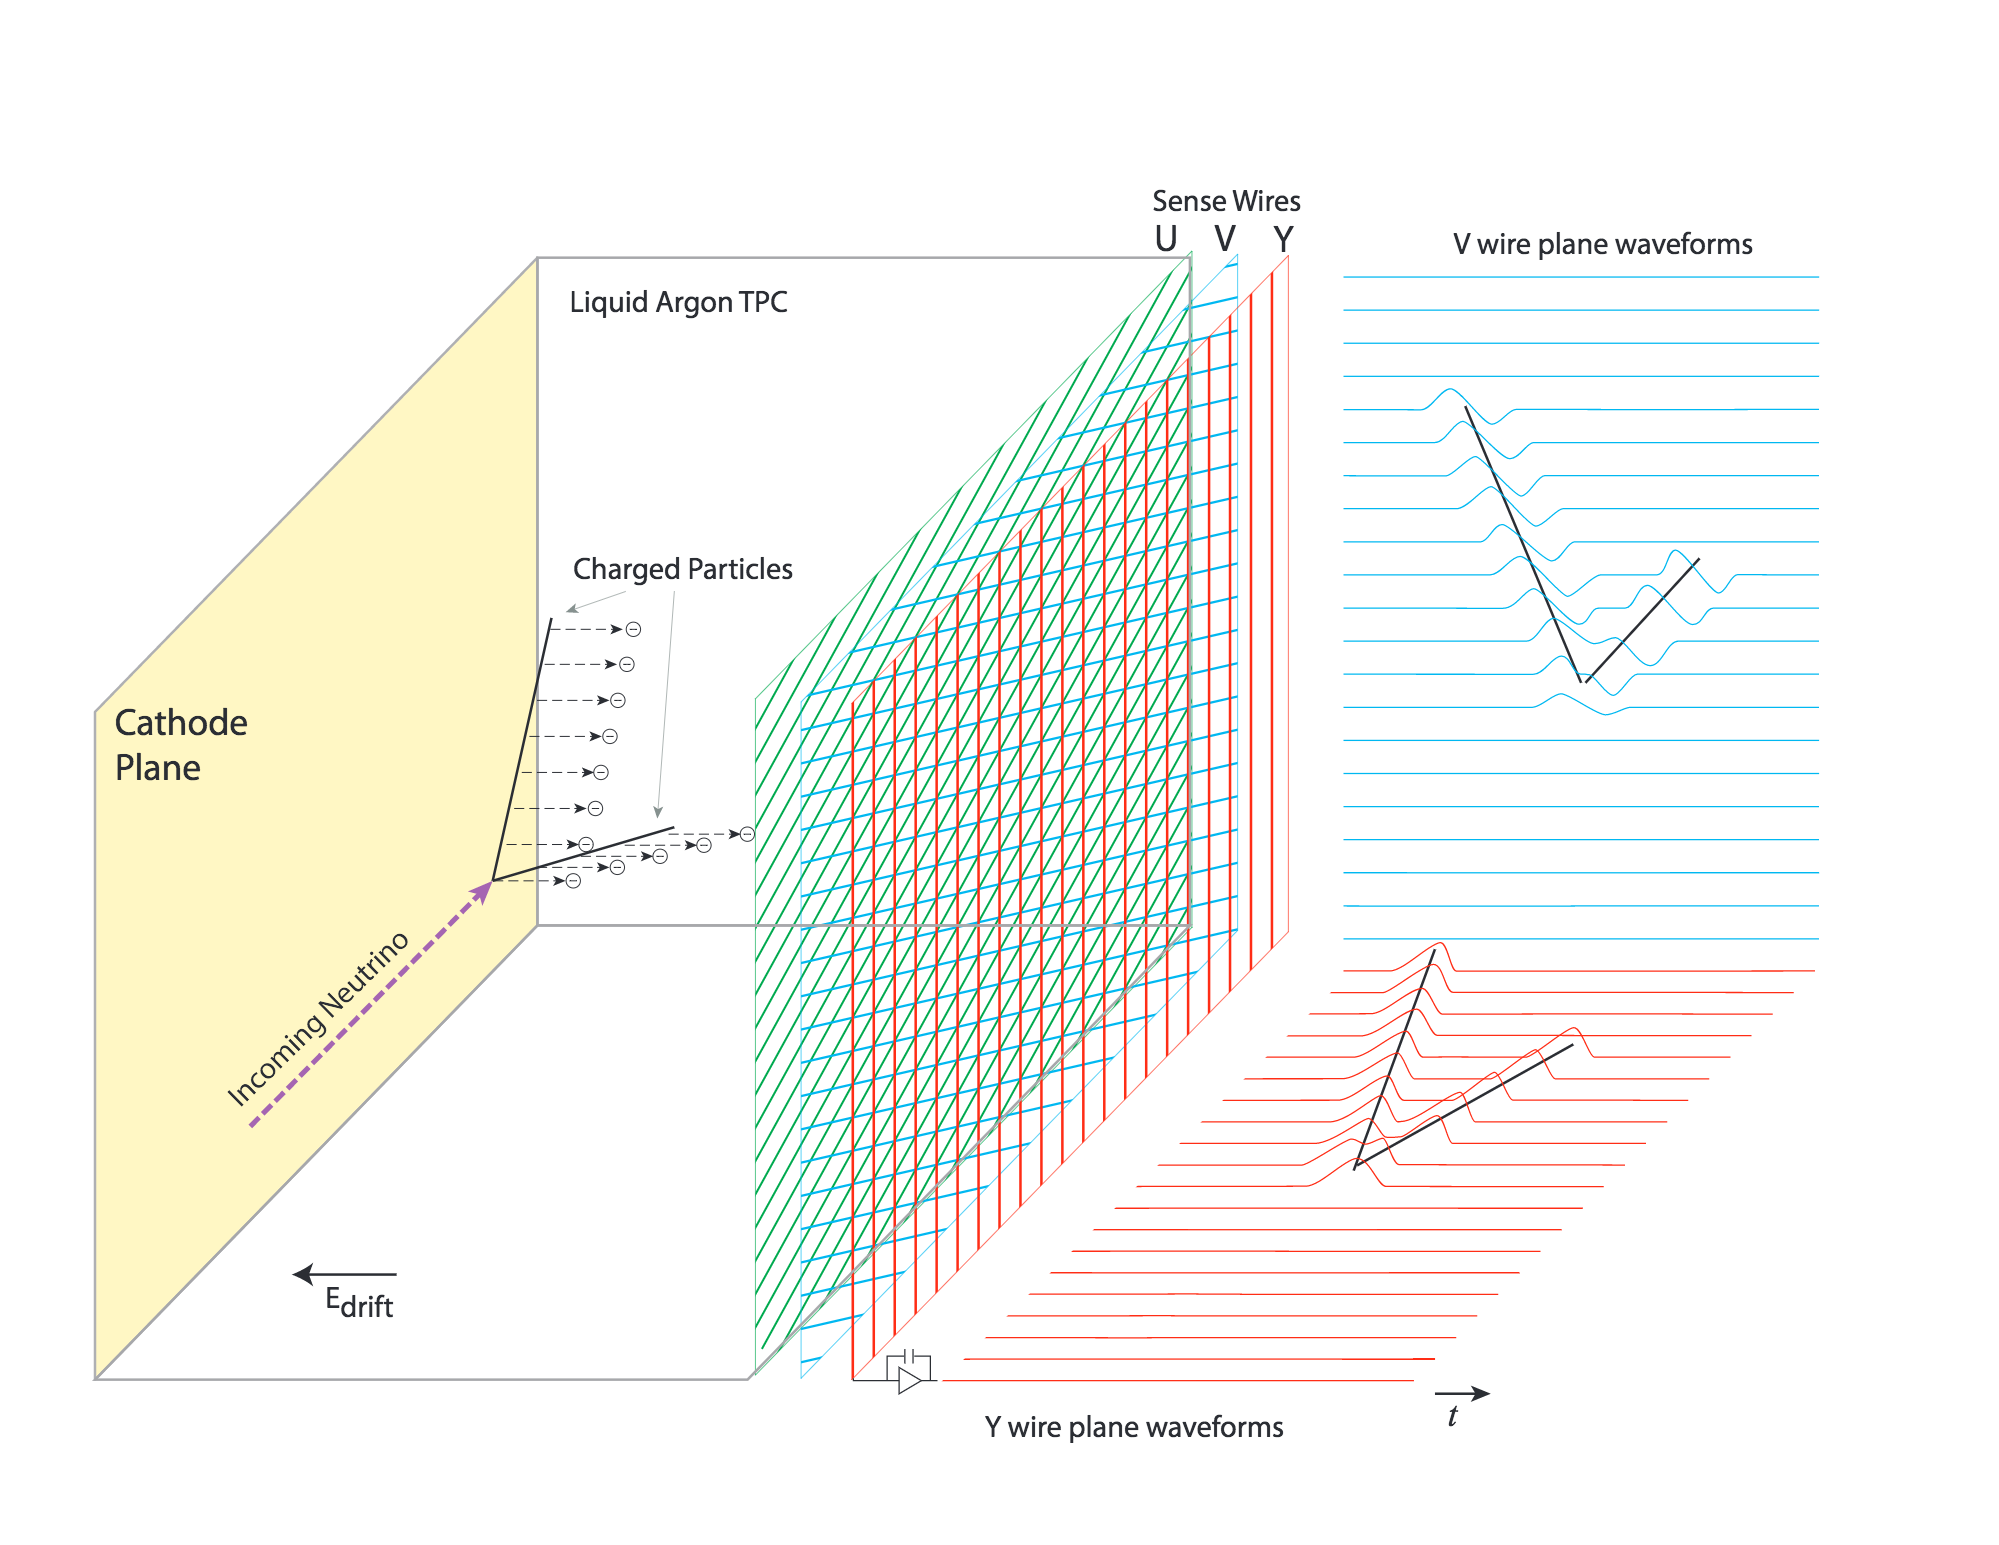
\includegraphics[width=0.9\textwidth]{Figures/LArTPC_concept.png} \\
\caption{\textit{A cartoon schematic of how a LArTPC works. Ionization electrons from particles traversing the detector medium are drifted by an electric field, $E_{\text{drift}}$ past multiple planes of sense wires. The signals on those wires create several two-dimensional images of the event, which are combined to create a three-dimensional reconstruction of the event. Note that in a LArTPC, PMTs are used to collect scintillation light, but are not drawn in this diagram.}}\label{LArTPC_concept_fig}
\end{figure}


\section{Time Projection Chamber}
The time projection chamber (TPC) used in the MicroBooNE experiment is a rectangular prism with dimensions 2.3 m vertical $\times$ 2.6 m horizontal $\times$ 10.4 m length (along the beam direction). The 8256 stainless steel sense wires forming the anode planes have a plane-to-plane spacing of 3 mm, and the wires on each plane are separated with a 3 mm wire pitch. The wires are connected to application-specific integrated circuits (ASICs) which operate at liquid argon temperatures. There are three wire planes. The first two planes (from the point of view of drifting electrons) each consist of 2400 wires and are induction planes, at angles $\pm60$ degrees relative to the vertical. The third wire plane consists of 3456 wires and is a collection plane, with vertically oriented wires. The electric field is created by a series of 64  2.54 cm diameter stainless steel pipes shaped into a rectangular loop held in place by a frame built of G10, forming the field cage. The negatively charged cathode is held at a high voltage (operating voltage is 70kV), and this voltage is incrementally stepped down across the field cage tubes with a voltage divider chain, with an equivalent resistance of 250 M$\Omega$ between each tube. The distance from center-to-center of adjacent field cage loops is 4 cm. This creates a uniform electric field within the LArTPC. A 3D rendering of the MicroBooNE TPC within the cryostat is shown in Figure \ref{cryo_3D_rendering_fig}. A summary of the MicroBooNE LArTPC design parameters and nominal operating conditions are described in Table \ref{UB_TPC_stats_table} \cite{UBDetectorPaper}.


\begin{figure}[ht!]
\centering
	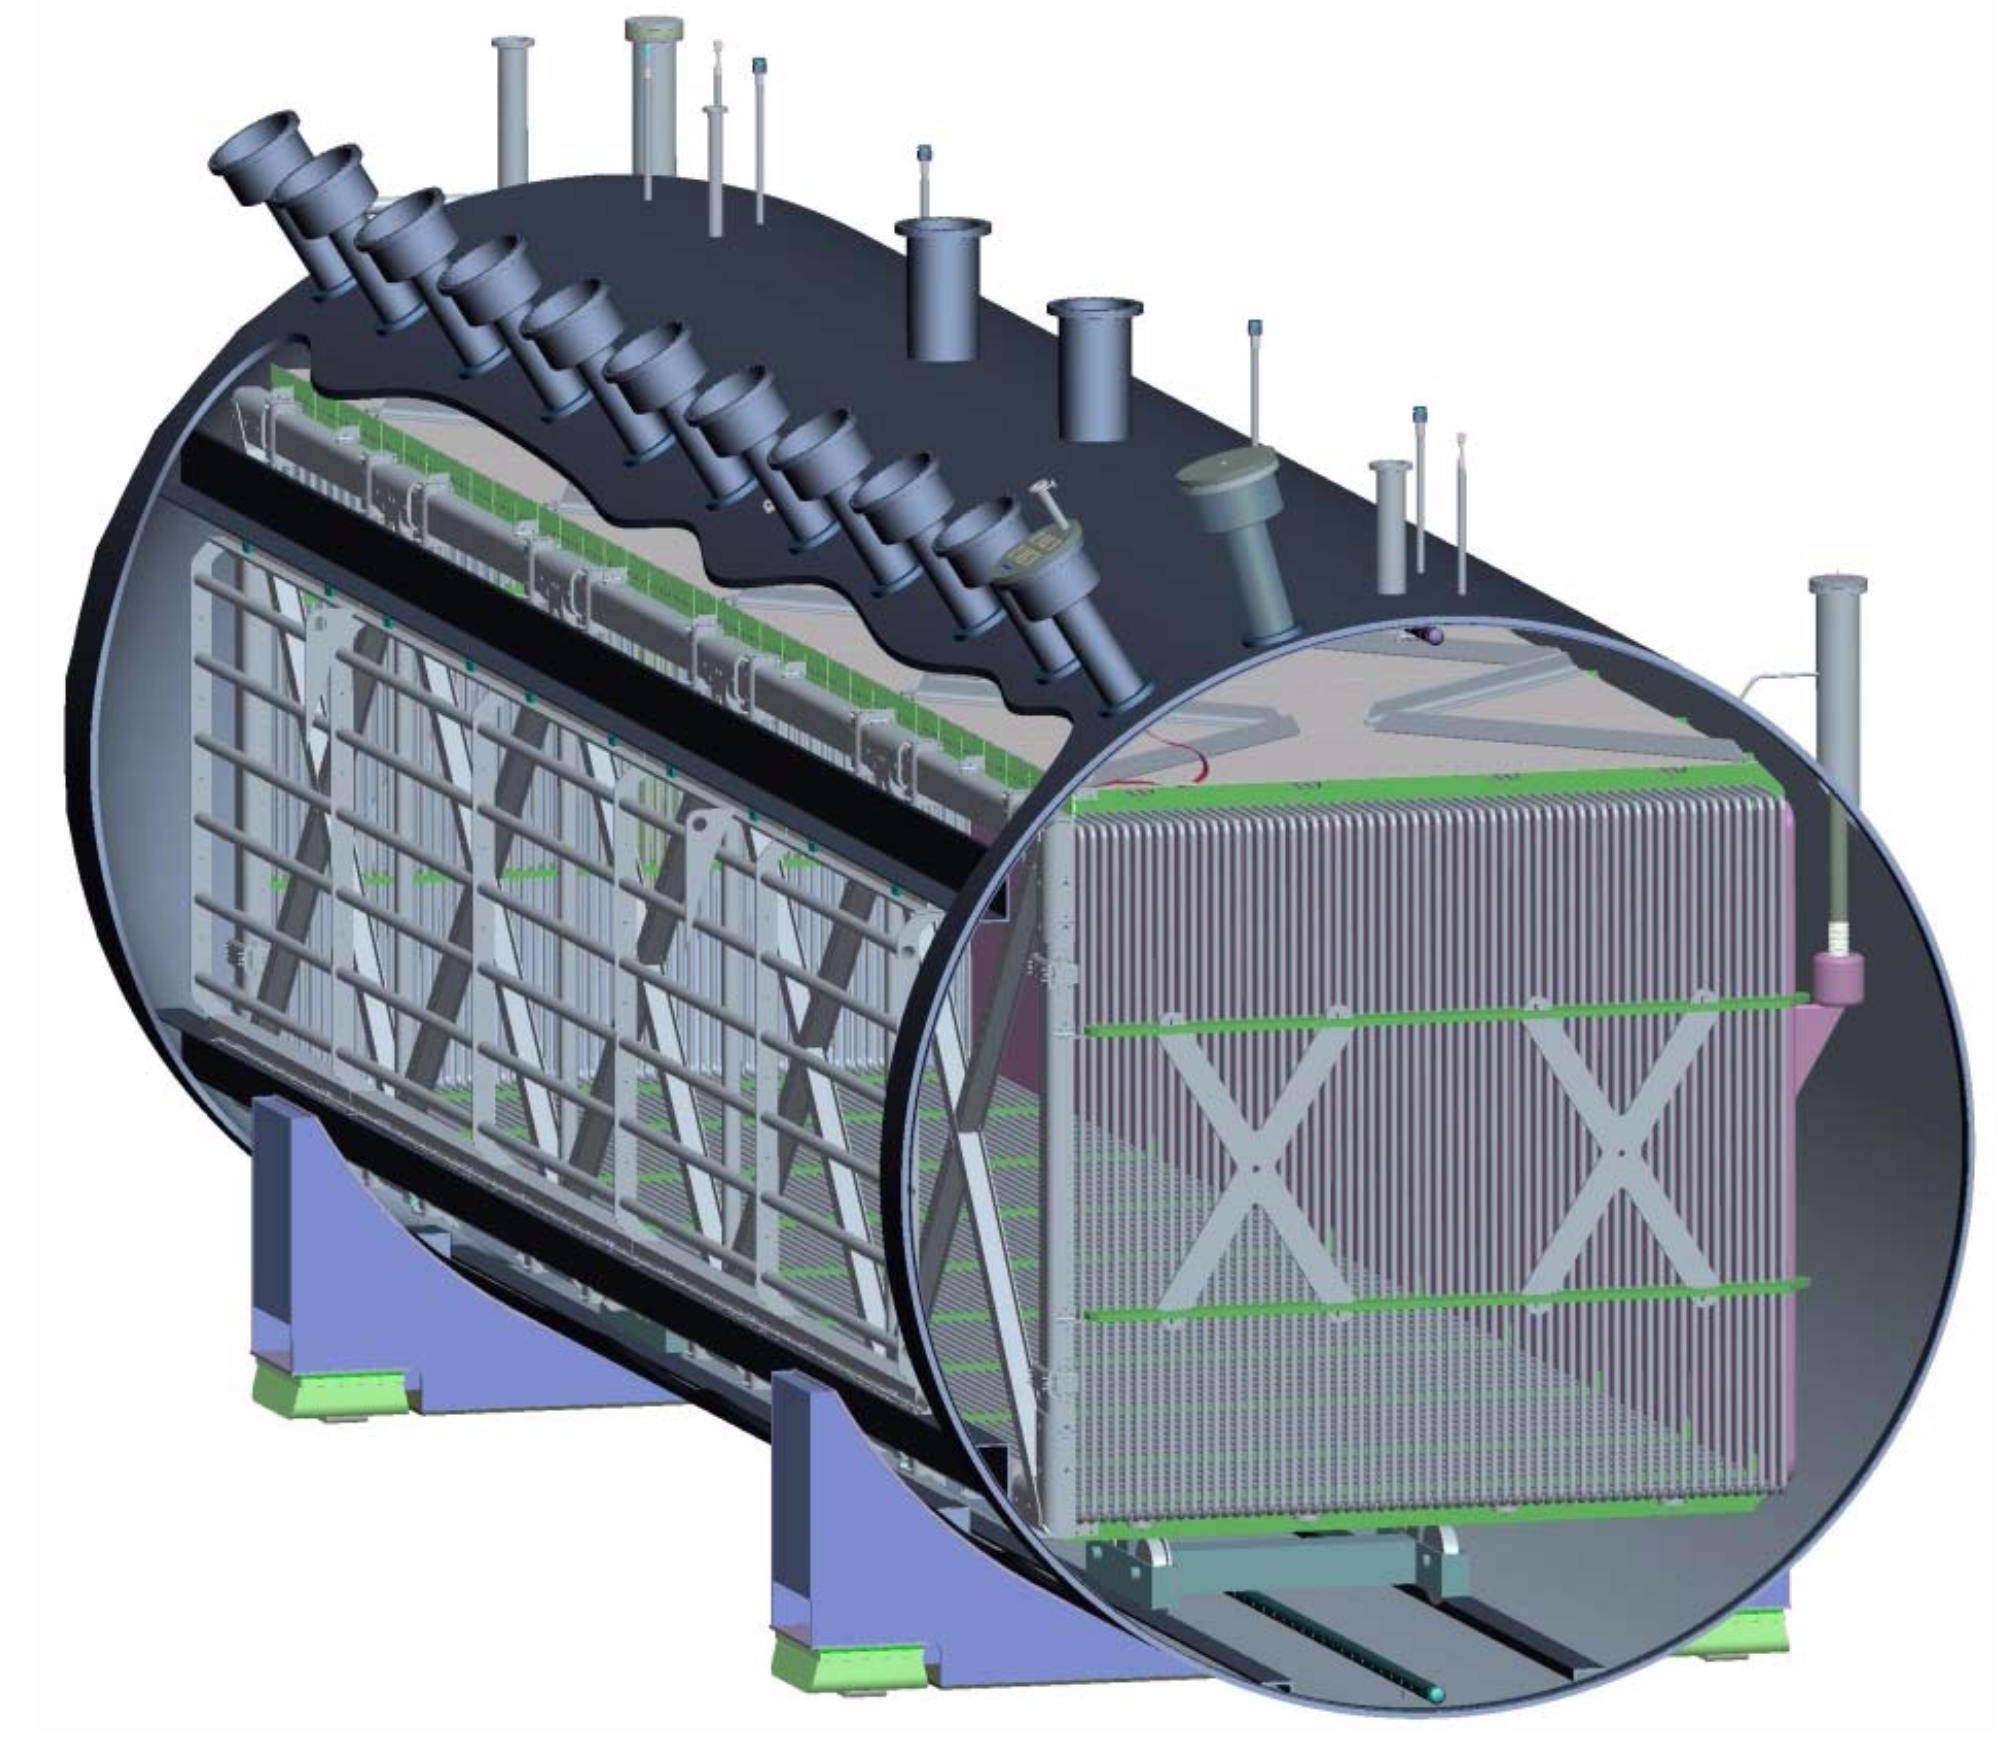
\includegraphics[width=0.7\textwidth]{Figures/cryo_3D_rendering.png} \\
\caption{\textit{A 3D rendering of the MicroBooNE detector. The rectangular time projection chamber (TPC) fits within the cylindrical cryostat. The feedthroughs along the top allow for the PMT and sense wire signals to be read out to the DAQ. Not shown are the photomultiplier tubes (PMTS) located on the wall behind the sense wire planes.}}\label{cryo_3D_rendering_fig}
\end{figure}


\begin{table}[!htb]
   \centering
     \caption{MicroBooNE LArTPC design parameters and nominal operating conditions.} 
    \begin{tabular}{lr} % Column formatting, @{} suppresses leading/trailing space
    \hline
    Parameter & Value \\
    \hline
    %\lartpc (active) dimensions ($h\times w\times l$) & 2.325 m $\times$ 2.560 m $\times$ 10.368 m\\
    %\lartpc (active) mass & 90 tons\\
   % \hline
    $\#$ Anode planes & 3\\
     Anode planes spacing& 3 mm \\
     Wire pitch & 3 mm  \\
     Wire type & SS, diam. 150 $\mu$m\\
     Wire coating & 2$\mu$m Cu, 0.1$\mu$m Ag\\
     Design Wire tension & 6.9N $\pm$ 1.0N\\
     $\#$ wires (total) & 8256 \\
     $\#$ Induction plane (U) wires & 2400 \\
     $\#$ Induction plane (V) wires & 2400 \\
     $\#$ Collection plane (Y) wires & 3456 \\
     Wire orientation (w.r.t. vertical) & +60$^{\circ}$,-60$^{\circ}$,0$^{\circ}$ (U,V,Y) \\
     \hline
     Cathode voltage (nominal) & -128 kV \\
     Bias voltages (U,V,Y) & -200 V, 0 V, +440 V \\
     Drift-field & 500 V/cm\\
   %  U-V gap field & 666.7 V/cm \\
    % V-Y gap field & 1466.7 V/cm \\
     Max. Drift Time, Cathode to U (at 500 V/cm) & 1.6 ms\\
    \hline
    $\#$ Field-cage steps & 64\\
    Ring-to-ring voltage step & 2.0 kV\\
    \hline
   \end{tabular}
   \label{UB_TPC_stats_table}
\end{table} 



\section{Light Collection System}
An important ingredient to the ultimate 3D reconstruction of particle interactions within a LArTPC is the light collection system. While the wire signals alone suffice to reconstruct 3D interactions, the absolute timing of the event (referred to as $t_0$) is unknown so there is ambiguity in the drift direction. Since the time scale with which scintillation light is created and propagates (nanoseconds) is orders of magnitude faster than that with which ionization electrons drift (milliseconds), measuring this light allows to clarify this ambiguity to high precision. Additionally, the scintillation light from interactions is relatively localized, and therefore combining the measured PMT signals with the physical position of the signal allows to match individual flashes of light with different interactions, which may have different $t_0$s. This is important to help tag and reject cosmic-induced backgrounds which may arrive outside of the expected beam neutrino arrival times.\\

The light collection system in MicroBooNE consists of 32 8-inch diameter Hamamatsu R5912-02mod cryogenic PMTs. These PMTs are mounted in a plane behind the three sense wire planes. The physical location of these PMTs is shown in Figure \ref{pmt_placement_fig}. These 32 PMTs provide 0.85\% photocathode coverage. Each PMT has mounted in front of it an acrylic plate, as shown in Figure \ref{pmt_mount_fig}. This plate is coated with TPB, an organic fluor which serves as a wavelength-shifting material. TPB absorbs the VUV scintillation light photons (128 nm wavelength in liquid argon) and re-emits it at visible wavelengths detectable by the PMTs, peaked at 425 nm.

\begin{figure}[ht!]
\centering
	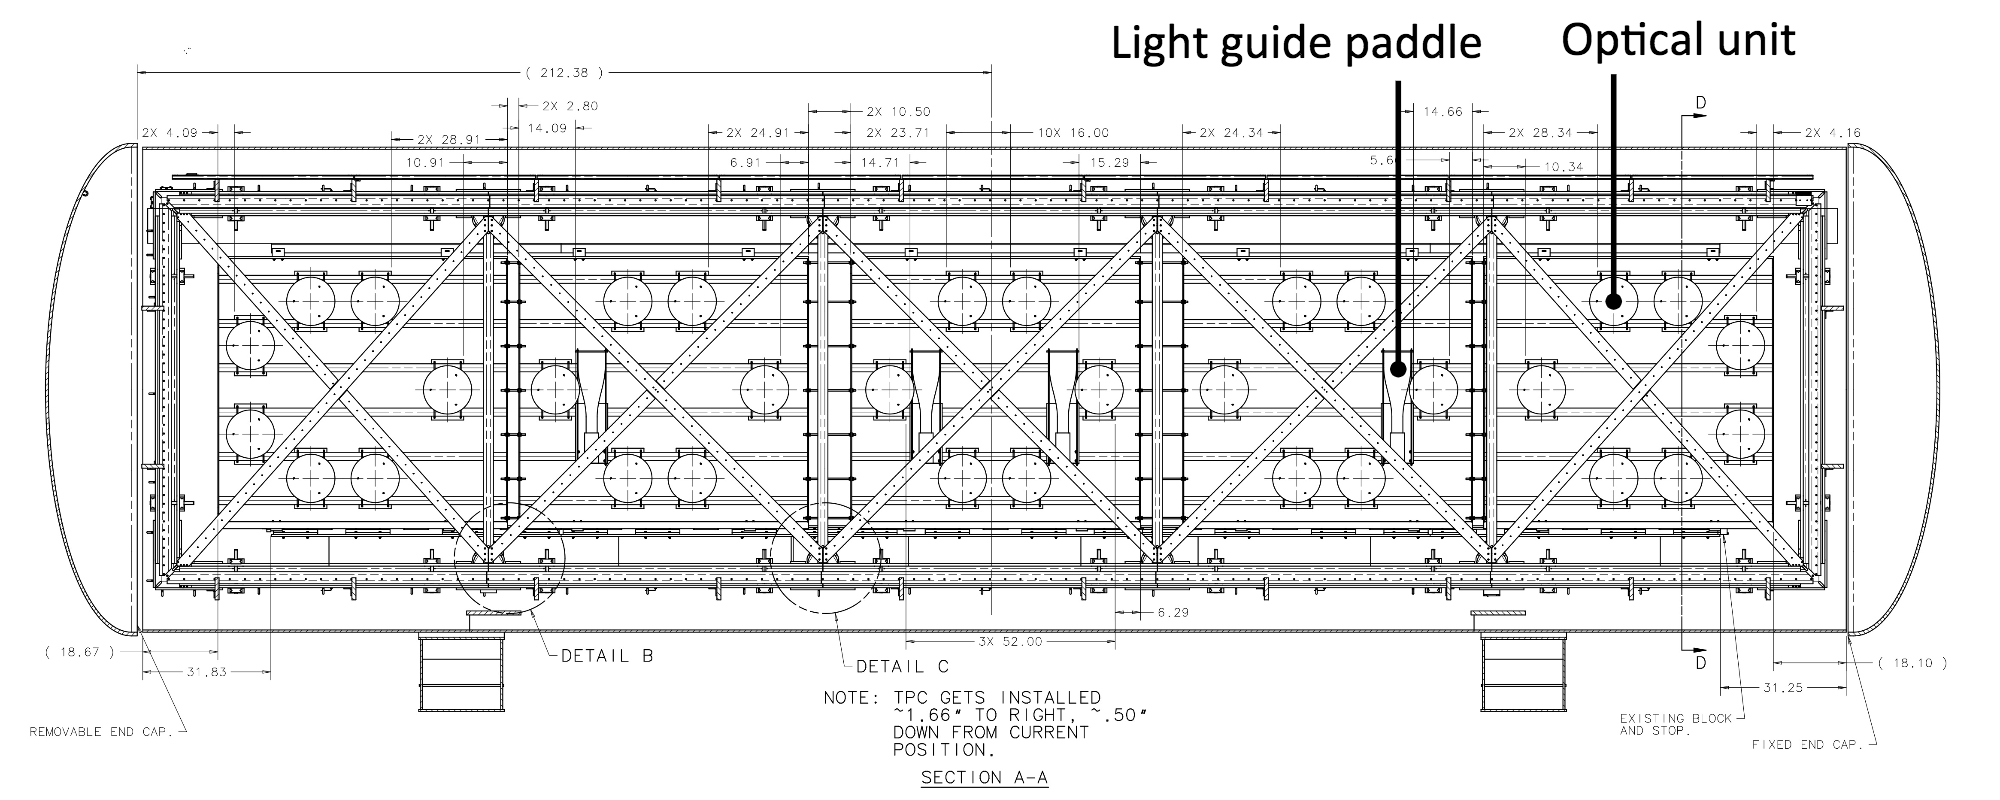
\includegraphics[width=0.9\textwidth]{Figures/pmt_placement.png} \\
\caption{\textit{A side-on view of the MicroBooNE detector showing the location of the 32 PMTs (labeled ``optical units'') and the four light guide paddles.}}\label{pmt_placement_fig}
\end{figure}


\begin{figure}[ht!]
\centering
	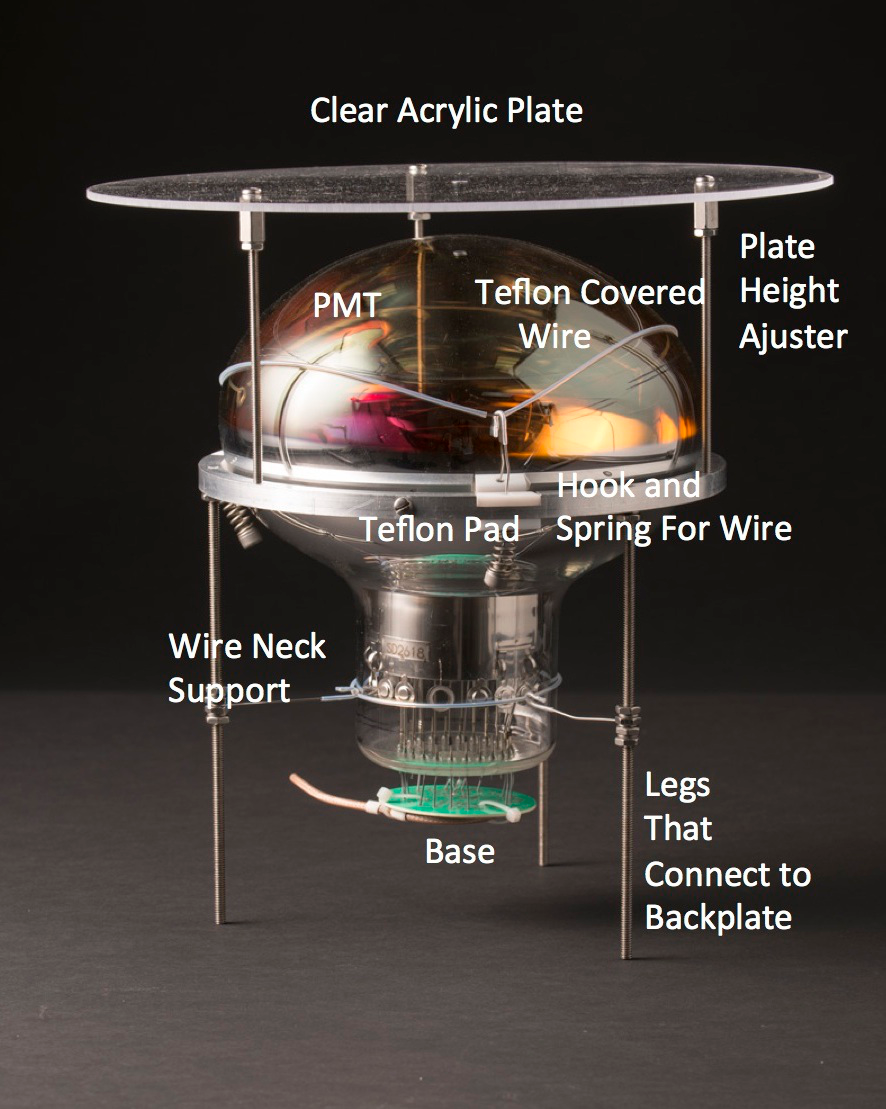
\includegraphics[width=0.6\textwidth]{Figures/mount_PMT_labeled.png} \\
\caption{\textit{A picture of one of the 8 inch Hamamatsu R5912-02mod cryogenic photomultiplier tubes (PMT) used in the MicroBooNE detector. Note the clear acrylic plate, which is coated with a wavelength-shifting organic fluor (TPB) before installation to convert the VUV liquid argon scintillation light into the visible spectrum, detectable by the PMT.}}\label{pmt_mount_fig}
\end{figure}


\section{Electronics, Readout, and Triggering}
Both of the two main subsystems of the MicroBooNE LArTPC (the TPC sense-wire planes and the optical PMTs) create analog signals which must be read out and digitized for use in analyses. This process involves amplification and shaping of the signals, and ultimately ends with the data acquisition (DAQ) software writing the digitized data to disk. While the readout is designed to have an additional data stream that continually writes to disk (designed with the hopes of measuring neutrino interactions from a potential future supernova explosion), the primary data stream reads out and stores signals only for a brief period of time when a hardware trigger is issued. The specifics of the readout and triggering for MicroBooNE are discussed in this section.\\

A schematic overview of the TPC and PMT signal processing and readout stages is shown in Figure \ref{readout_scheme_fig}. The analog signals from the 8256 sense wires in the TPC pass through CMOS analog front end ASICs which operate on cold motherboards at liquid argon temperatures. The signals are then shaped and amplified by cold intermediate amplifiers before passing through a warm feed-through. The signals are received by custom-designed LArTPC readout modules distributed over nine readout creates, which digitize the signals and process them. The TPC wire signals are digitized at 16 MHz and then down-sampled in the digitization process to 2 MHz. The TPC system reads out four 1.6 $ms$ frames of wire signal data associated with one event. This time is chosen based on how long it takes ionization electrons from the cathode side of the TPC to drift to the anode wires (roughly 1.6 $ms$ depending on drift field). Reading out one frame before a trigger is issued, along with two frames after ensures enough data is available to identify both a neutrino interaction, as well as all cosmic ray signals that arrive soon enough before or after the neutrino which need to be reconstructed in analyses.\\

\begin{figure}[ht!]
\centering
    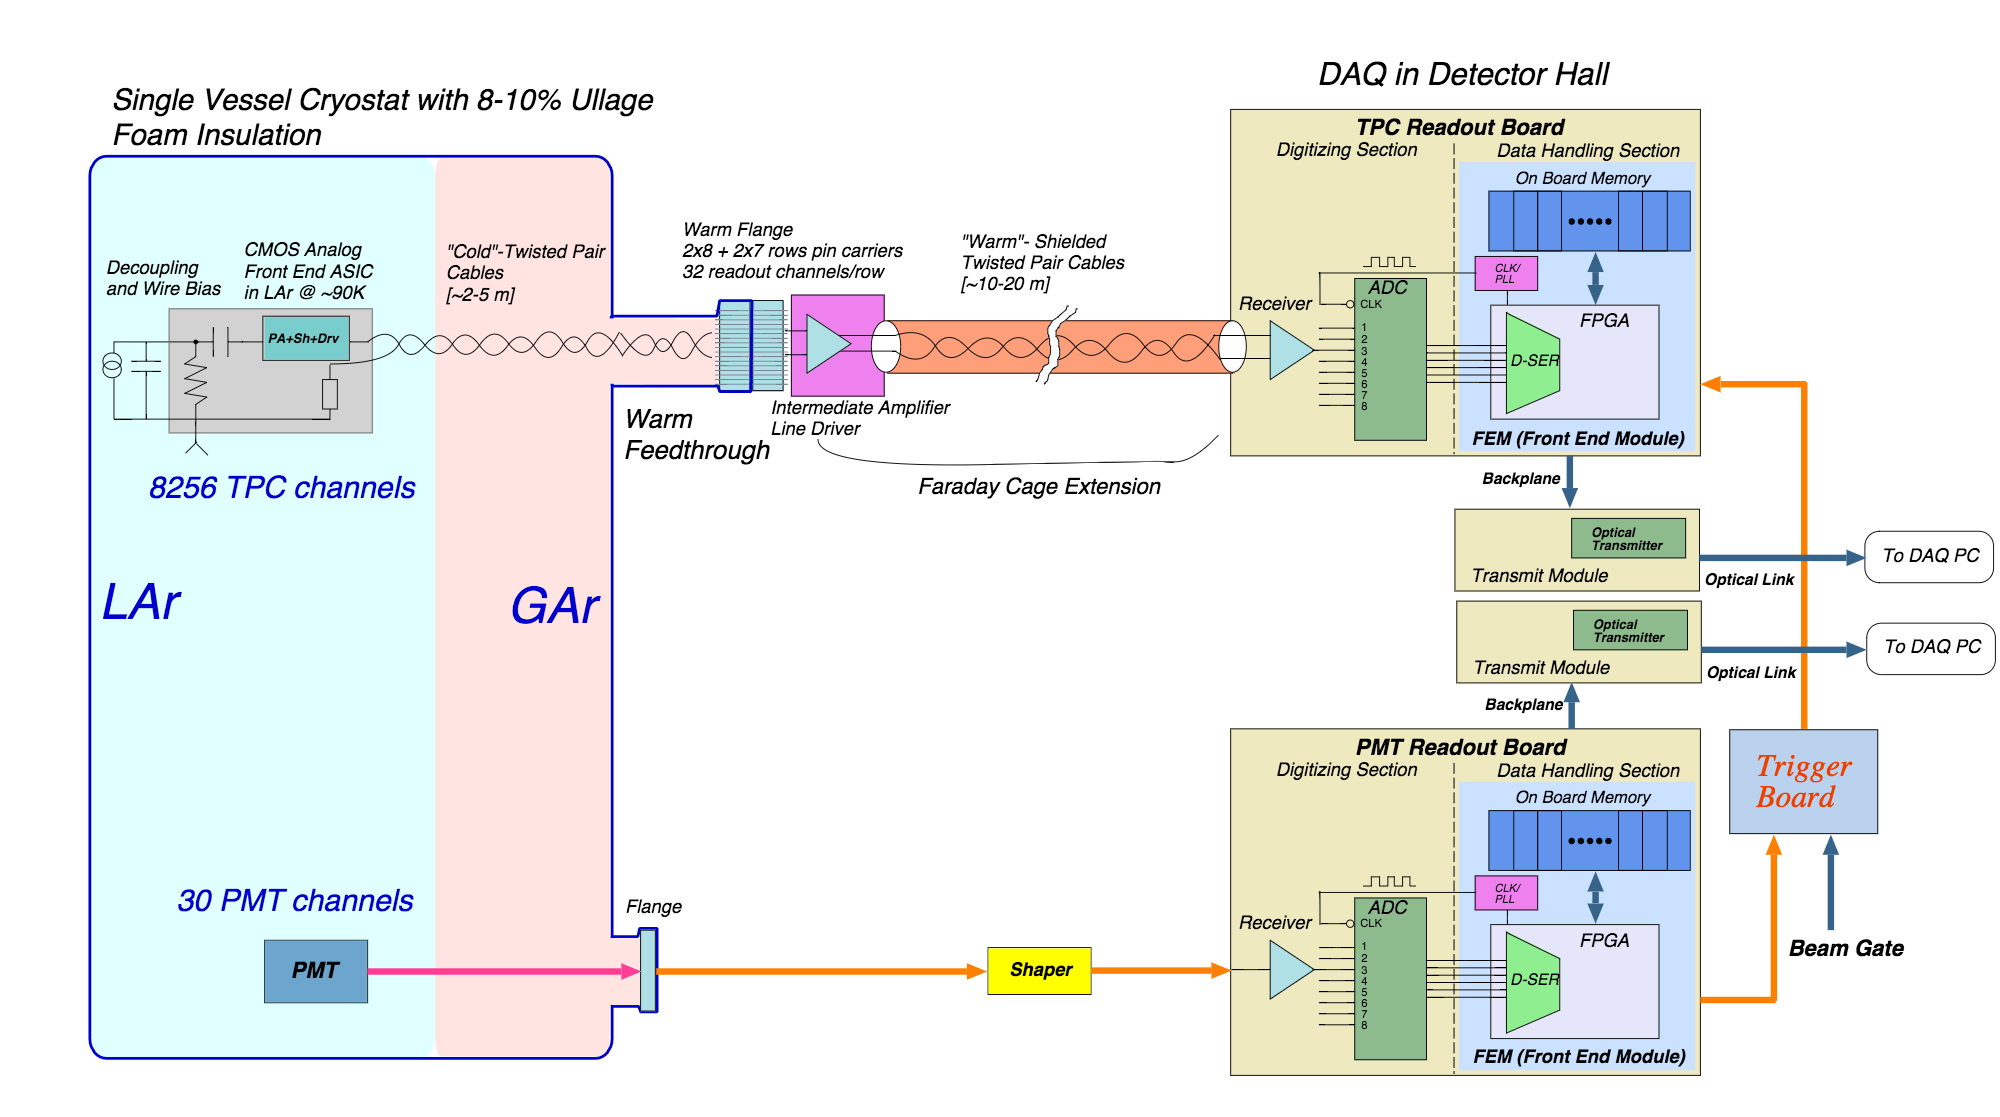
\includegraphics[width=0.95\textwidth]{Figures/UB_readout_scheme.png} \\
\caption{\textit{The MicroBooNE readout schematic. On the left are portions of the readout operating at argon temperatures. Signals pass through feedthroughs into warm electronics readout boards, unique for the TPC (sense wire signals) and the light collection system (PMT signals). These signals are combined with external timing signals from the accelerator to form triggers that initiate readout of all systems.}}\label{readout_scheme_fig}
\end{figure}

A similar process occurs for the PMT signals. The PMT signals undergo separate shaping with a 60 $ns$ peaking time to allow for digitization of several samples on the rising edge of a signal for more precise timing reconstruction abilities. The PMT signals are digitized at 64 MHz, but are not read out continuously during the same $4 \times 1.6$ $ms$ TPC readout time; only shaped PMT signals above a small discriminator threshold are read out and stored for later reconstruction. The PMT signals are split into high- and low- gain channels, to extend the dynamic range of the ADC.\\

The readout of both TPC and PMT systems are initiated by triggers formed in a separate trigger board located in a warm electronics readout crate. While many different triggers are used by MicroBooNE, the one relevant for this analysis is the BNB trigger. To form this trigger, a timing signal from the BNB accelerator is shaped and fed into the trigger board. The FPGA firmware in the PMT front end readout modules generates a PMT trigger when PMT signal multiplicity is greater than 1 and summed PMT pulse-height is more than 2 photo-electrons summed over all of the high gain PMT channels. If a PMT trigger is issued by the firmware in coincidence with the $1.6 \mu s$ beam gate window from the accelerator, a BNB trigger is generated by the trigger board. This trigger signal is fanned-out to all readout crates (TPC and PMT), instructing them to initiate a readout simultaneously. Once the readout is complete, the data from each readout crate is packaged and shipped to the DAQ software, which assembles all of the data into one event in memory, which is saved to disk and eventually used in reconstruction and analysis. Note that ultimately, the MicroBooNE collaboration has moved towards using a software- based trigger for its beam-based analyses.

%\cite{UBDetectorPaper}

\chapter{The Booster Neutrino Beam}
\label{sec:beam}
%http://neutrino.fnal.gov/events/summer_lecture_series/slides2016/Zarko-Pavlovic-Sources.pdf
%http://microboone-docdb.fnal.gov:8080/cgi-bin/RetrieveFile?docid=5787&filename=bnb-flux-microboone.pdf&version=4
The purpose of this chapter is to describe how the neutrinos studied in subsequently described analyses are produced in the Booster Neutrino Beam-line (BNB) at the Fermi National Accelerator Laboratory. An understanding of how these neutrinos are produced and their flux through the MicroBooNE detector is important to properly interpret the results of the low energy excess analysis and kaon production analysis, described in Chapters \ref{sec:LEEsensitivity} and \ref{sec:LEEsensitivity}. In describing the neutrino production techniques and sources, the reader will be introduced to the systematic uncertainties associated with the neutrino source, both in terms of how they arise, and their magnitude. 

\section{The Booster Neutrino Beam}\label{beam_descript_section}
The Boost Neutrino Beam-line (BNB) collides protons at 8.89 GeV/c momentum from the Fermilab Booster synchrotron with a beryllium target to produce a high flux of neutrinos. The layout of the BNB is shown in Figure \ref{BNB_layout_schematic}, and the relevant steps of the neutrino production process will be described in the following sections.

\begin{figure}[ht!]
\centering
	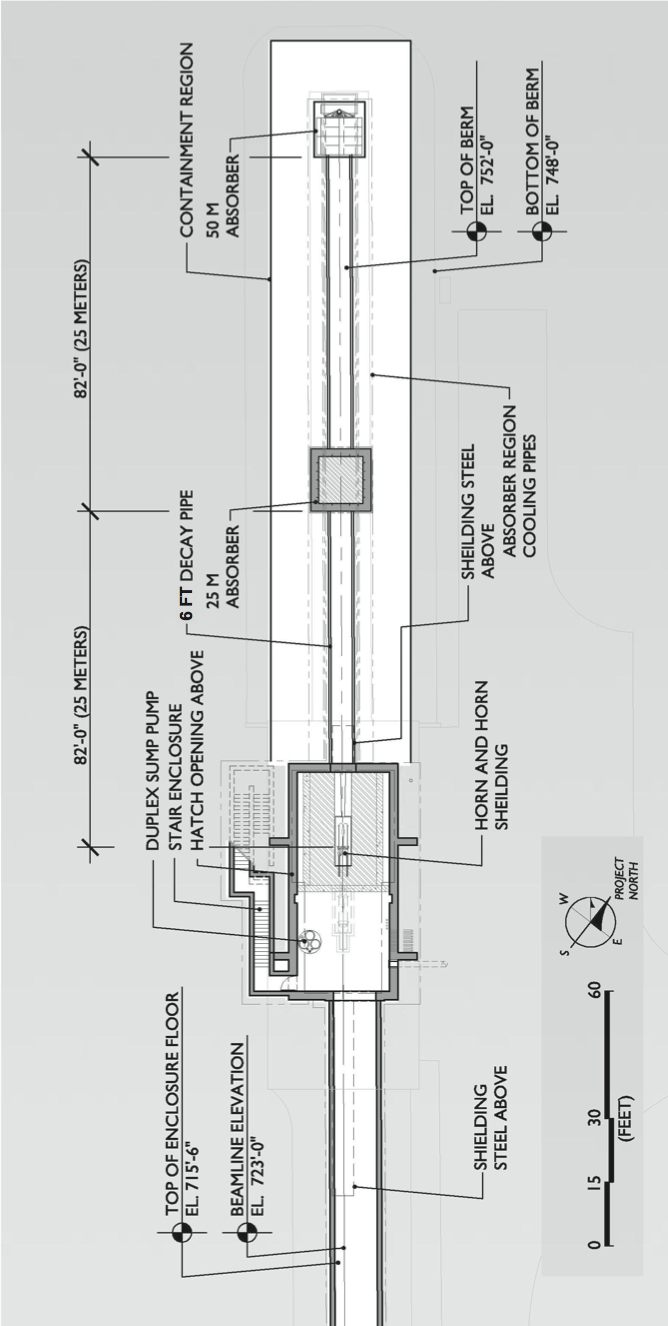
\includegraphics[width=0.5\textwidth]{Figures/BNB_layout_schematic.png} \\
\caption{\textit{Overall layout of the BNB. The primary proton beam, extracted from the Booster, enters the target hall from the left. Upon exiting the target hall, particles encounter a 50-meter-long decay region, terminating in the beam stop on the right. Figure and caption from \protect\cite{MBFluxPaper}.}}\label{BNB_layout_schematic}
\end{figure}

\subsection{Primary Proton Beam}
The protons originate from $H_2$ gas molecules converted to $H^-$ ions via a Cockroft-Walton generator, which are initially accelerated up to approximately 1 MeV kinetic energy. These ions are subjected to a linear accelerator using alternating electromagnetic fields to increase their energy to about 400 MeV. Passing through a carbon foil removes electrons, and the bare protons enter the Booster synchrotron where they are accelerated up to 8.89 GeV/c momentum. The protons are bunched in ``beam spills'' containing roughly $4\times10^{12}$ protons spaced throughout a 1.6 $\mu s$ time window. The protons are then directed towards a thick beryllium target.\\

The absolute number of protons directed on target (POT) is measured by two toroids upstream of the target which part of a larger beam monitoring system. The error on the POT is on the order of 2\%. Additional beam characteristics are monitored by beam position monitors (BPMs), a multi-wire chamber, and a resistive wall monitor (RWM) which together measure beam intensity, timing, width, position, and direction.

\subsection{Proton Target and Focusing Horn}
The beryllium target is 71.1 cm long, which corresponds to 1.7 proton interaction lengths, and is 0.51 cm in radius. Beryllium is chosen as the proton target because it's relatively low Z (4) minimizes radiative losses from the protons before their p-Be interactions which produce secondary mesons ($\pi^\pm$, $K^\pm$, $K^0_L$).\\

The beryllium target is located within a larger focusing electromagnet, referred to as the horn. A schematic drawing of the horn is shown in Figure \ref{BNB_horn_schematic}. The horn is an aluminum alloy pulsed toroidal electromagnet. The pulsed current has a peak at 170 kA and width in time of 143 $\mu s$, coincident with the proton beam arrival time on the target. The current flows along the inner conductor, then returns along the outer conductor. The electromagnetic fields created by this current serve to focus the charged secondaries produced in the p-Be interactions. The direction of this current can be switched to focus the positively charged secondaries, or the negatively charged secondaries, ultimately producing a beam of primarily neutrinos (``neutrino mode'') or of primarily antineutrinos (``antineutrino mode'') respectively.

%\ref{BNB_numode_fig}



\begin{figure}[ht!]
\centering
	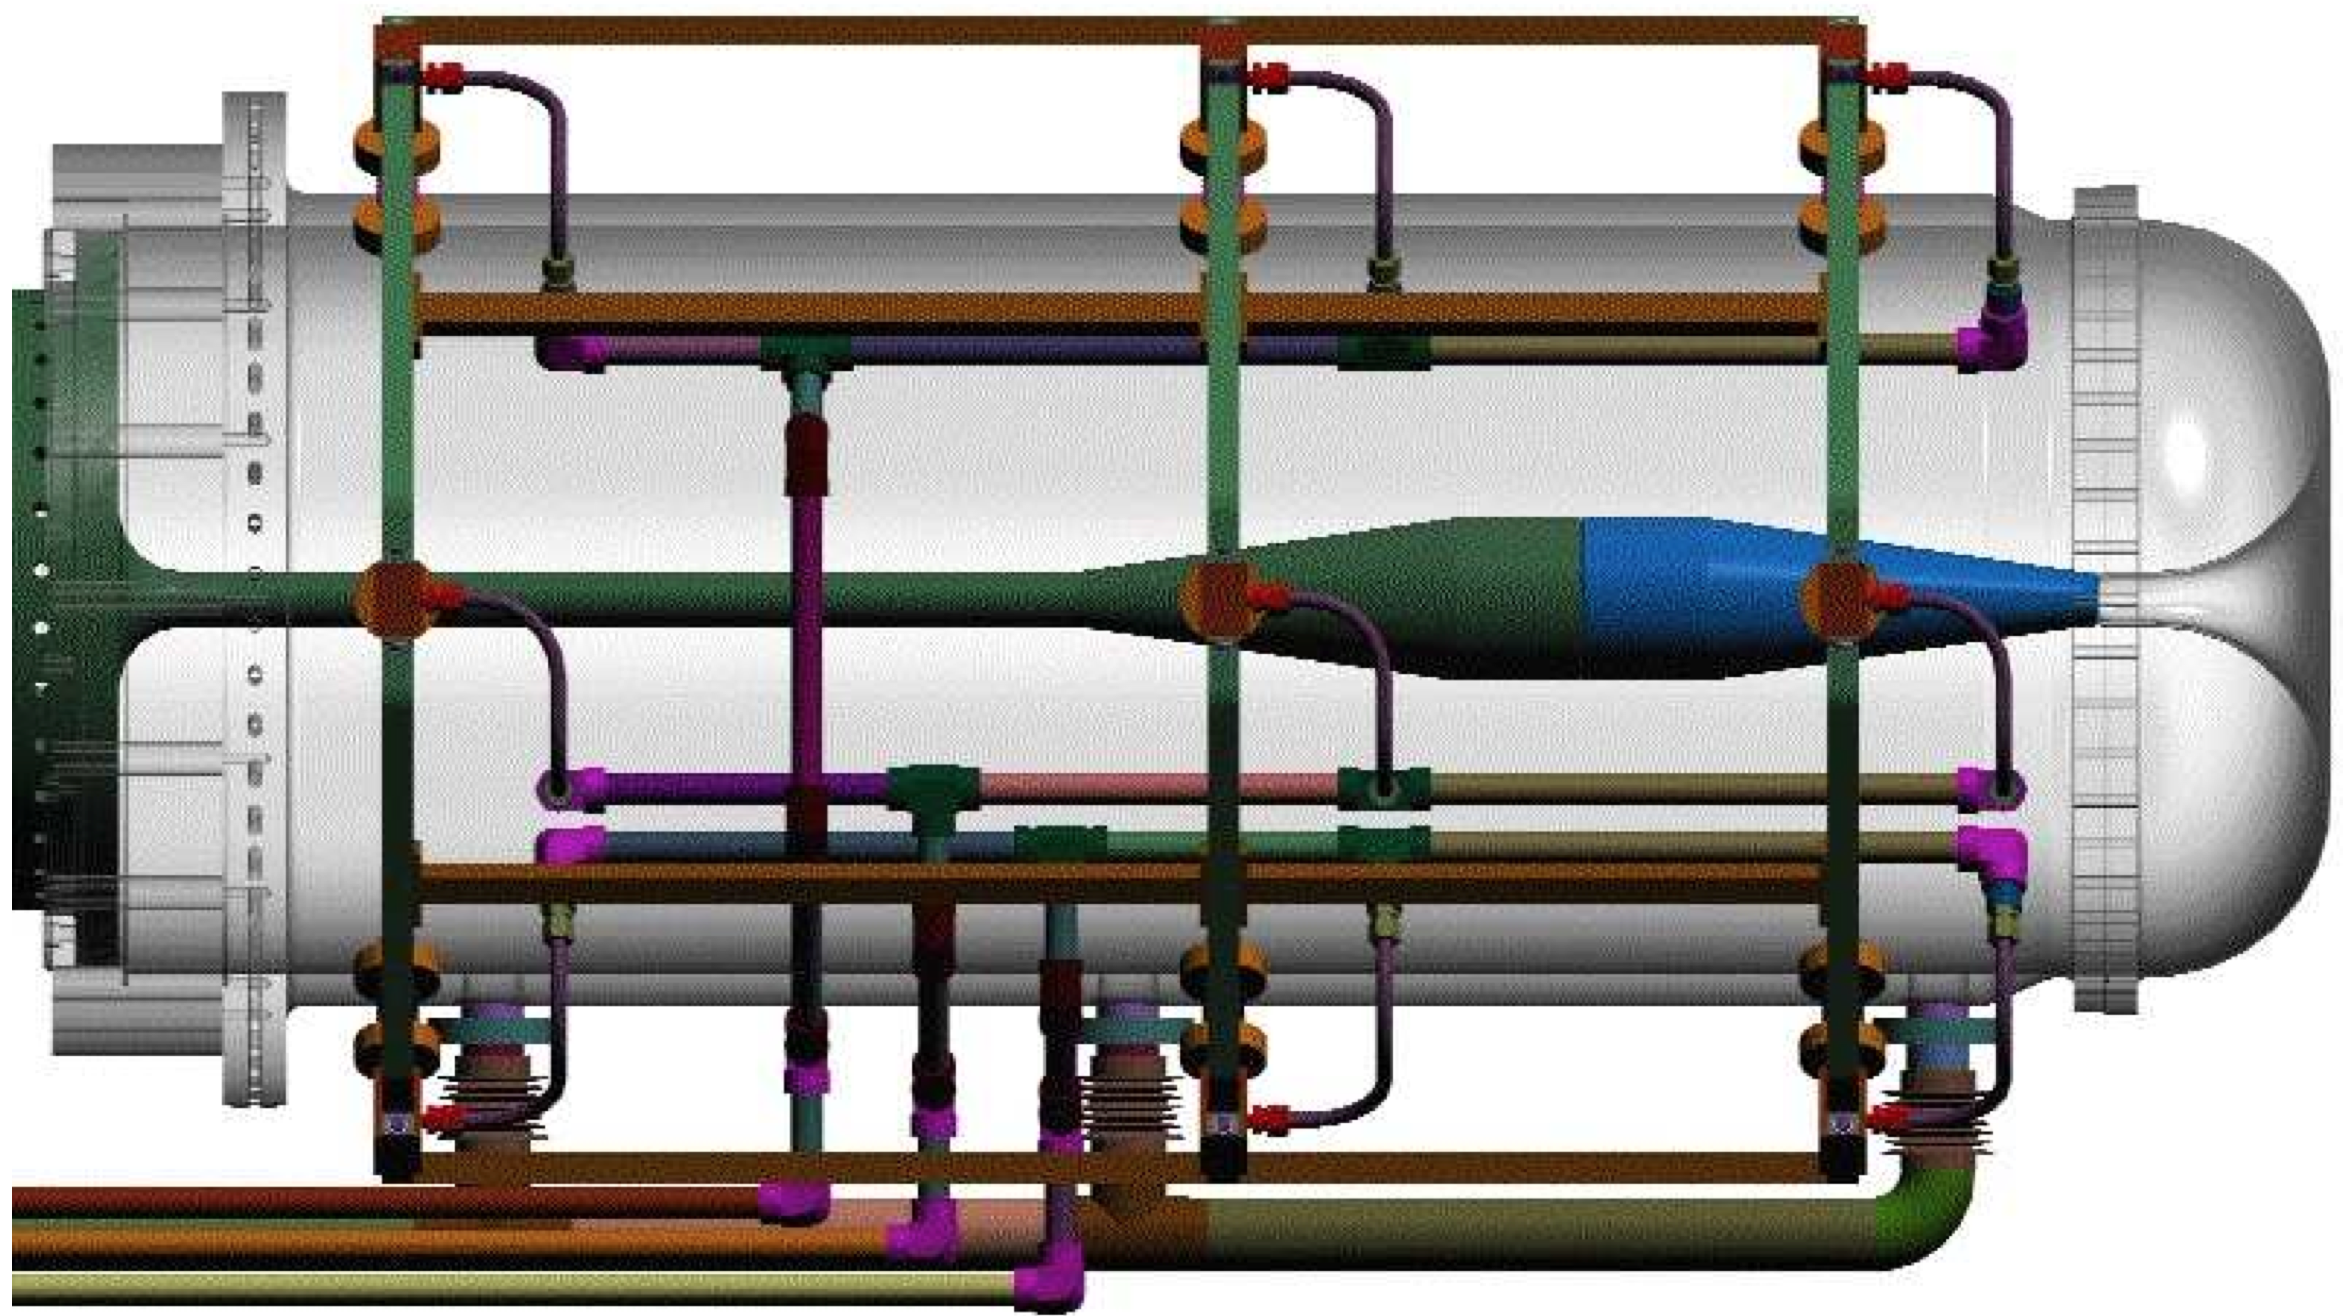
\includegraphics[width=0.7\textwidth]{Figures/BNB_horn_schematic.png} \\
\caption{\textit{The BNB focusing horn system. The gray outer conductor is drawn transparent for visualization purposes. The beryllium target lies within the central hollow tube axis. A current flows along the inner conductor, returning along the outer conductor.}}\label{BNB_horn_schematic}
\end{figure}


\begin{figure}[ht!]
\centering
	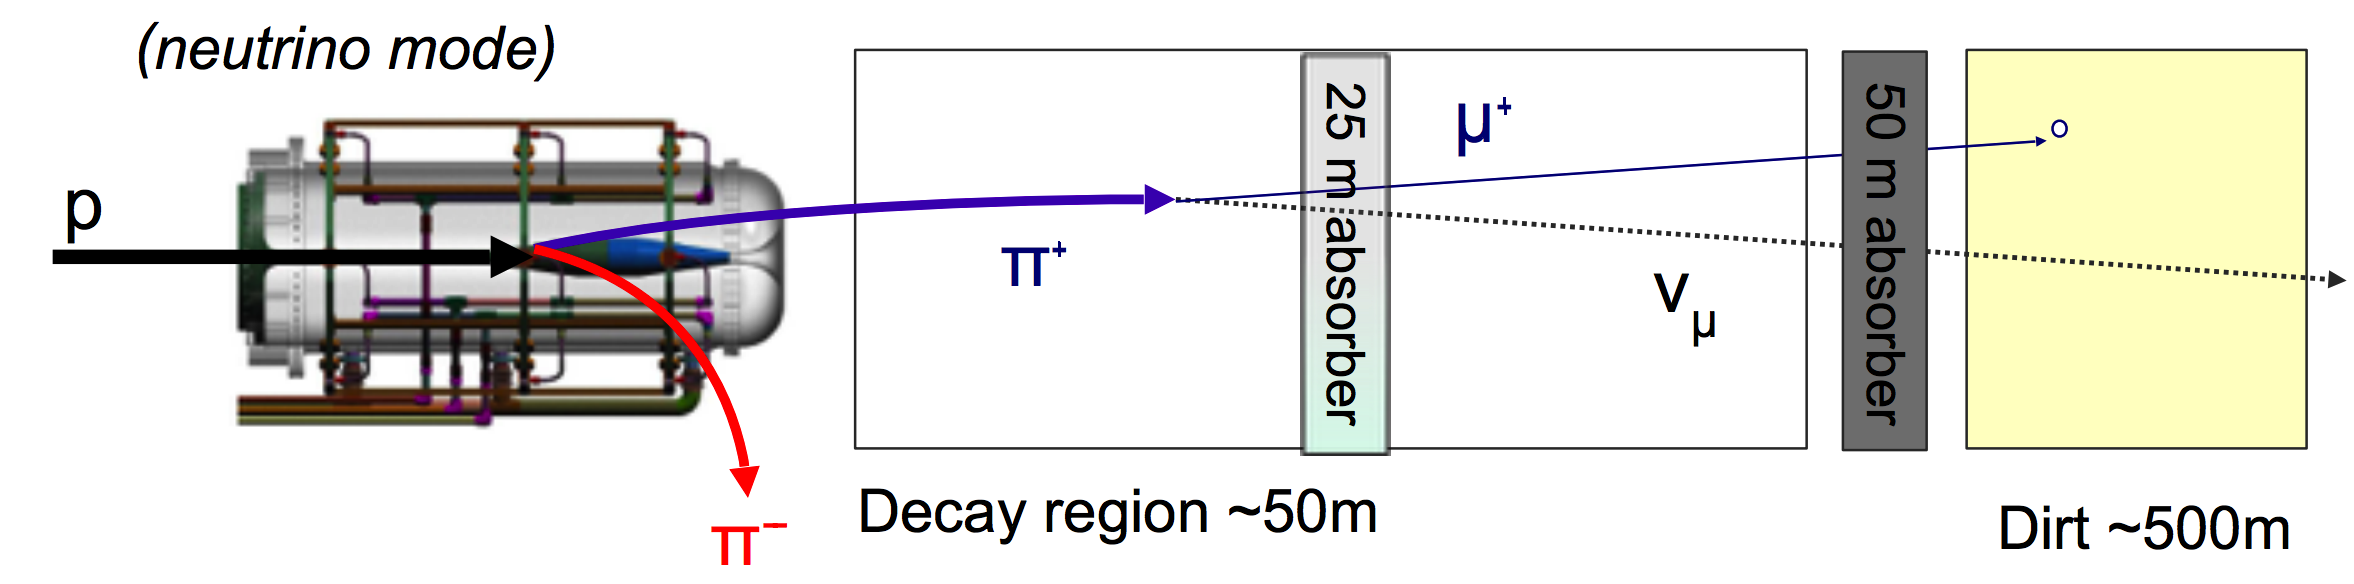
\includegraphics[width=1.0\textwidth]{Figures/BNB_numode_fig.png} \\
\caption{\textit{XXXcaption.}}\label{BNB_numode_fig}
\end{figure}



\section{Neutrino Flux Prediction}\label{beam_flux_descript_section}


\chapter{Low Energy Excess Sensitivity Studies}
\label{sec:LEEsensitivity}
\section{Low Energy Excess Overview and Motivation}
\subsection{Introduction}
The purpose of this chapter is to describe the MicroBooNE analysis centered around measuring the observed low energy excess as seen by its predicessor experiment, MiniBooNE. This chapter begins with a historical motivation for this analysis by describing the LSND experiment which first observed an excess of $\overline{\nu_e}$ in a $\overline{\nu_\mu}$. Then, a detailed description of the MiniBooNE experiment (detector and analysis) is provided, which observed an unexplained excess of electron-like events in the neutrino energy region between 200 to 475 MeV.\\

With historical context in perspective, this chapter then discusses an analysis conducted which determines the sensitivity of the previously described MicroBooNE detector to measure the same signal as MiniBooNE, assuming that signal originated from an excess of beam-induced $\nu_e$ interactions. This discussion covers the signal modeling which comes from MiniBooNE published data releases, the event selection and background mitigation techniques in MicroBooNE, and ultimately the expected sensitivity to measure such a signal.

\subsection{LSND Observation}
%Brief discussion of the LSND experiment and how they saw an excess of antinue in the antinumu beam with L/E that didn't fit in with any measured mixing angles and delta m2 in 3 neutrino model.

In 2001, the Liquid Scintillator Neutrino Detector (LSND) collaboration published an observation of excess events consistent with $\overline{\nu_e}$ interactions above the expected background in an $\overline{\nu_\mu}$ beam at the Los Alamos Neutron Science Center \cite{LSNDPaper}. The $\frac{L}{E}$ ($\approx$ $\frac{30 m}{40 MeV}$) for this excess disagreed with previous measurements of neutrino mixing angles and $\Delta m^2$ values in the three neutrino model. The LSND excess corresponded to a $\Delta m^2$ of approximately 1 $eV^2$, significantly higher than previously measured values of $\Delta m_{12}^2$ and $\Delta m_{23}^2$. One explanation for this drastically different $\Delta m^2$ value is the existance of potential additional ``sterile'' neutrino states, which must not interact weakly given the Z- boson decay width constrains the number of weakly interacting neutrino states to three.\\
To test the LSND result, the MiniBooNE experiment was designed. It would similarly measure $\nu_e$ interactions in a primarily $\nu_\mu$ beam, with a similar $\frac{L}{E}$ ($\approx$ $\frac{500m}{700 MeV}$).



\subsection{The MiniBooNE Experiment}

\subsubsection{The MiniBooNE Detector and Monte Carlo Simulation}

%Description of the detector, a schematic figure, description of cherenkov rings, the location of the detector in the BNB. Discussion of how they use NUANCE, mention they use identical beam simulation and reweighting (reweighting should be covered in the beam chapter).


The MiniBooNE detector \cite{MBDetectorPaper} consists of a spherical tank located 541 meters downstream of the BNB neutrino production target, with diameter of 12.2 meters filled with 818 tons of mineral oil underneath at least 3 meters of earth overburden as shown in Figure \ref{MB_detector_fig}. As seen in the figure, there exists an opaque barrier separating a veto region and a signal region. The walls of the signal region are painted black to reduce re-scattering of light and are instrumented with 1280 8-inch photomultiplier tubes (PMTs), most of which were reused from the LSND experiment. In the signal region, the photocathode coverage is 11.8\%. This region is intended to identify beam neutrino interactions happening within it; the PMTs face radially inwards. The veto region is 35 cm thick and is instrumented with 240 PMTs which face tangent to the detector radius and its purpose is to reject backgrounds coming from outside of the detector (cosmics, which have a rate at the detector location of about 10 kHz). The inner surface of the veto region is coated in a reflective paint. The efficiency for rejecting cosmic ray muons with the outer veto region was measured to be 99.99\%.\\

\begin{figure}[ht!]
\centering
	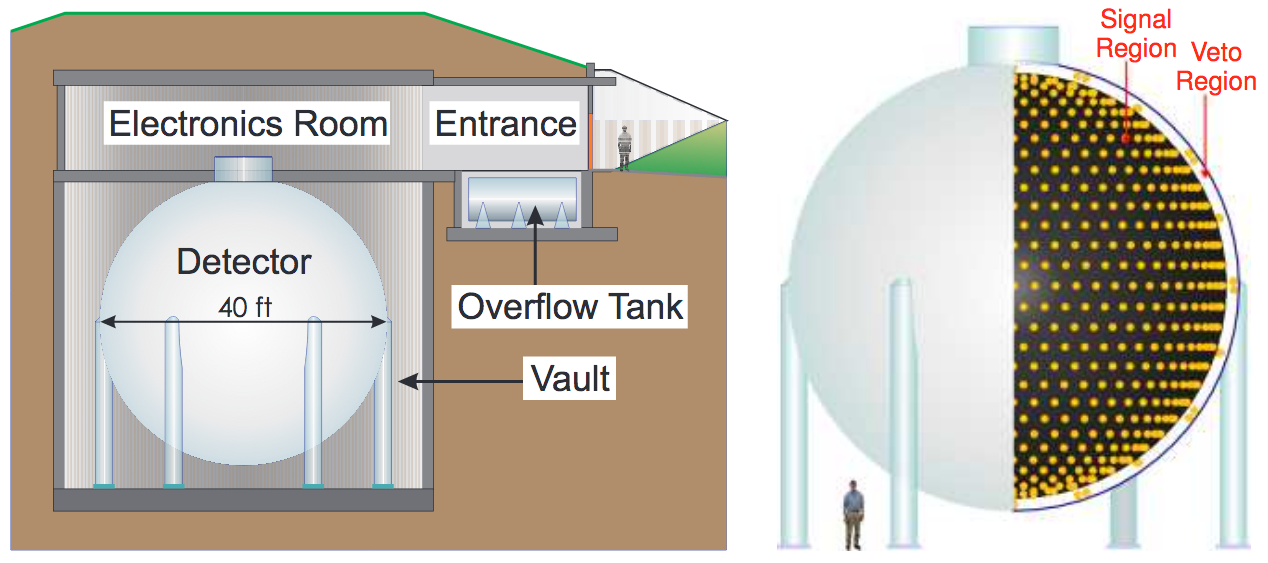
\includegraphics[width=0.9\textwidth]{Figures/MB_detectorpaper_fig.png} \\
\caption{\textit{The MiniBooNE detector enclosure (left) and a cut-away drawing (right) of the detector showing the distribution of PMT's in the signal and veto regions.}}\label{MB_detector_fig}
\end{figure}

The detection method of the MiniBooNE experiment is based primarily on Cherenkov light. The mineral oil within the signal region acts as the neutrino target material. The majority of final state particles exiting neutrino interactions at neutrino energies from the BNB are produced above Cherenkov threshold. These particles produce Cherenkov light which is detected by the PMTs lining the signal region of the detector. Reconstructing the pattern this light projects onto the walls of the signal region allows for some particle identification abilities.\\

Thie mineral oil used in MiniBooNE is Marcol 7 Light Mineral Oil ($CH_2$). While the oil has lower density than water (a common material choice for Cherenkov detectors) and therefore smaller probability of a neutrino interacting within the detector, the other benefits outweigh this downside. The oil has good light transmission throughout the wavelength range of 320 nm to 600 nm, relatively large refractive index (1.47, greater than water at 1.33), and its long extinction length of greater than 20 m for 420 nm light. This extinction length allows for loss of no more than 25\% of light generated by a neutrino interaction at the center of the detector. Additionally, the Cherenkov threshold is lower than that of water for the final state particles of interest (electrons, pions, muons, protons), allowing for the measurement of lower energy particles.\\

The PMTs have a wavelength dependent efficiency with a peak at 390 nm, with half that efficiency at 315 and 490 nm. They are operated at +2000 V which results in a gain of approximately $1.6 \times 10^7$. They have an intrinsic time resolution on the order of 1 ns, which is the dominant contribution to the final time resolution in the final PMT data after readout through data acquisition (DAQ) electronics. The DAQ reads out a pmt when the charge signal corresponds to more than 0.1 photoelectrons (PE). The deadtime between successive PMT readouts is on the order of 250 ns after the first readout began. PMT charge and timing information is stored in intervals of 200 $\mu s$ following any trigger signal. The trigger signal of interest for this analysis is the beam trigger which is induced by the BNB accelerator clock such that the DAQ begins readout 5 $\mu s$ before each beam spill.\\

The detector is calibrated in situ primarily from cosmic ray muons. Within the detector are six optically sealed scintillator cubes. Incominb muons are tagged with a muon hodoscope above the detector with angular resolution better than 2 degrees. Those muons that stop within one of the scintillation cubes have well defined energy (in the 100-800 MeV range), as the stopping power of muons in mineral oil is well known, and therefore provide an energy calibration source. Additionally, the outgoing electrons from stopping muon decay (Michel electrons) have a well known endpoint of around 50 MeV and therefore serve as an electron energy calibration source at that energy. Through-going muons are also used as an energy calibration source at higher energies (above 1 GeV). Additional calibration sources include a laser system built into the detector, and reconstructed $\pi^0$ masses (with peak energy at 135 MeV).

\subsubsection{MiniBooNE Event Selection and Observed Excess}
% Brief description of their event selection cuts, mention that the energy definition they use is CCQE and they're looking specifically for CCQE topologies, description of what CCQE means. Figure of their results indicating the excess in neutrino mode. 

Different final state particles exiting a neutrino interaction in the MiniBooNE signal volume will create different patterns of Cherenkov light read out by the PMTs. Figure \ref{georgia_cherenkov_cartoon_fig} \cite{GeorgiaThesis} shows how these patterns differ for different common kinds of final state particles (muons, electrons/photons, and neutral pion decays). A muon track produces a crisp, filled-in ring of Cherenkov light, while an electron or photon produces a more fuzzy, hollow ring. A neutral pion decay will result in two photons. By reconstructing these patterns in the PMT data read out from a triggered event in MiniBooNE, the flavor and energy of the interacting neutrino can be determined. With this kind of detection technique it is important to note that a single photon signal is indistinguishable from that of a single electron signal, an important ingredient to the ultimate ambiguity of the observed low energy excess in MiniBooNE.\\

\begin{figure}[ht!]
\centering
	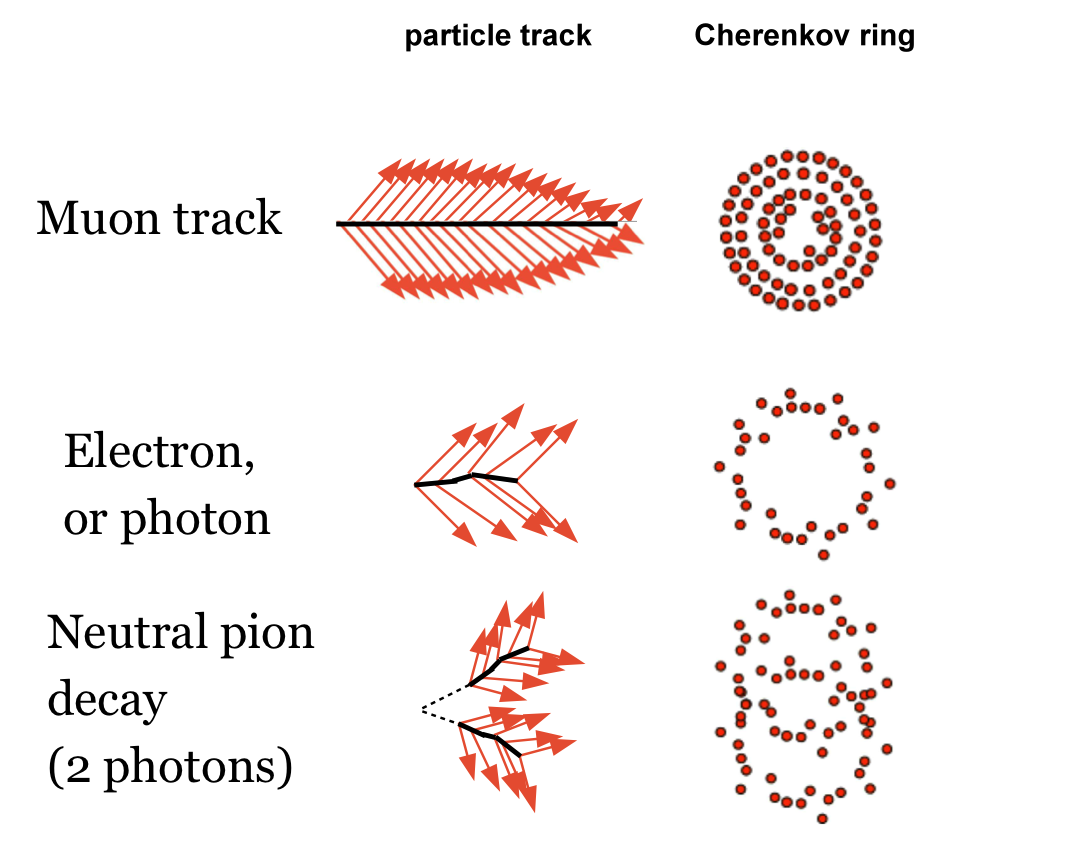
\includegraphics[width=0.9\textwidth]{Figures/georgia_cherenkov_cartoon.png} \\
\caption{\textit{A schematic of the pattern Cherenkov light from different particles would make projected onto the inner walls of the MiniBooNE detector. Top is a muon track (a filled-in ring), middle is an electron (a fuzzy ring), bottom is a photon that pair-produces and creates two fuzzy rings.}}\label{georgia_cherenkov_cartoon_fig}
\end{figure}

The topology of interest in the MiniBooNE oscillation search is that of charged-current quasi-elastic (CCQE) interactions, shown in Figure \ref{georgia_ccqe_feynman_fig}. This interaction channel is the dominant one in the neutrino energy range of the BNB, around 1 GeV $E_\nu$. In a $\nu_l$ CCQE interaction (where $l$ is the neutrino flavor), a lepton of flavor $l$ is produced, along with a proton. The single outgoing lepton is the characteristic event signature for which MiniBooNE searches.\\


\begin{figure}[ht!]
\centering
	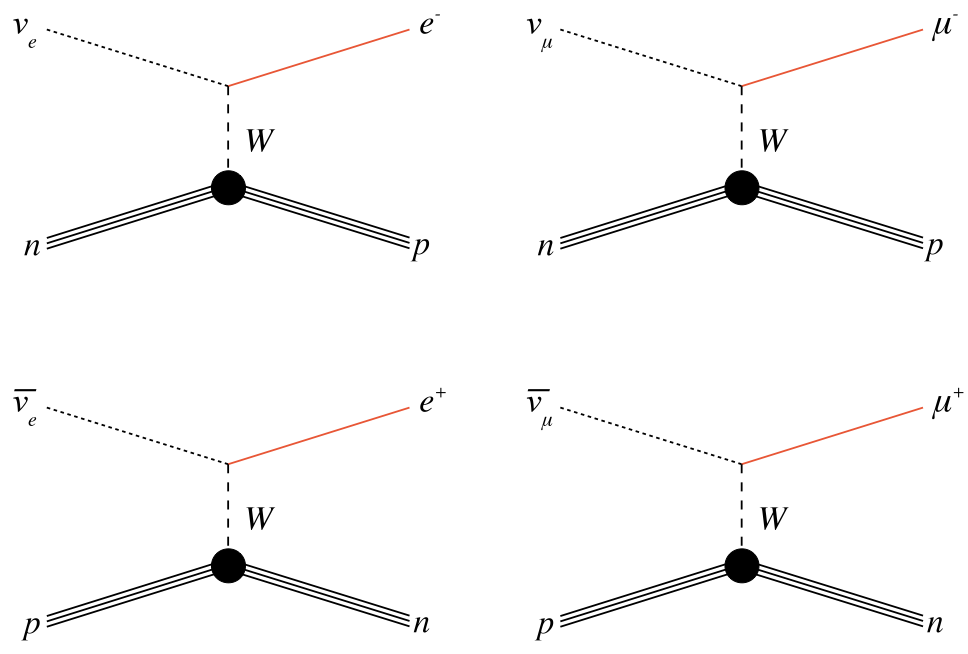
\includegraphics[width=0.9\textwidth]{Figures/georgia_ccqe_feynman.png} \\
\caption{\textit{Feynman diagrams of the charged-current quasi-elastic (CCQE) interaction channel for $\nu_e$, $\nu_\mu$, $\overline{\nu_\mu}$, and $\overline{\nu_e}$ (clockwise from the top left). $\nu_e$ CCQE is the signal channel for the MiniBooNE oscillation analysis.}}\label{georgia_ccqe_feynman_fig}
\end{figure}


In order to select $\nu_e^{CCQE}$ events, cuts are placed to mitigate backgrounds. The most powerful rejection comes from requiring the events occur within the beam timing window. Two additional cuts are used that require there be more activity within the signal volume than the outer veto volume, a signature characteristic of beam related neutrino events. These pre-cuts achieve more than a 99.99\% rejection of beam unrelated backgrounds.\\

In order to reconstruct events, MiniBooNE uses a maximum likelihood fitting algorithm leveraging properties of charged particle tracks inferred from measured charges and times on the PMTs. The likelihoods to different event hypothesis are used to classify each event as a signal $\nu_e$ CCQE event, or as a background process like $\nu_\mu$ CCQE and NC $\pi^0$ production. Note that MiniBooNE cannot differentiate between a $\mu^+$ and a $\mu^-$, or $e^+$ and $e^-$ so discrimination between neutrino and antineutrino on an event-by-event basis is impossible.\\

Assuming CCQE kinematics, the incident neutrino energy is reconstructed with knowledge of the outgoing lepton energy ($E_l$) and scattering angle ($\theta_l$). In MiniBooNE specifically, the struck nucleon is assumed to be at rest, so the incident neutrino energy $E_\nu^{CCQE}$ is given by:
\begin{equation}\label{MB_CCQE_formula}
E_\nu^{CCQE} = \frac{2m_nE_l+m_p^2-m_n^2-m_l^2}{2(m_n-E_l+\cos\theta_l\sqrt{E_l^2-m_l^2})}
\end{equation}
where $m_n$, $m_p$, $m_l$ are the masses of the neutron, proton, and lepton respectively, and $\theta_l$ is the scattering angle of the outgoing lepton with respect to the (known) beam neutrino direction.\\

With the described reconstruction methods and energy definition, the MiniBooNE published results \cite{MBLEEPaper} for the $\nu_e$ appearance search in neutrino mode running are shown in Figure \ref{MB_published_stackedhisto_fig}. There is clearly a statistically significant excess of events below $E_\nu^{CCQE}$ of 475 MeV. Note that besides the irriducible intrinsic $\nu_e$ backgrounds, the dominant background in the excess region is $\pi^0$ MID (red). In a $\pi^0$ MID event event, a $\pi^0$ is created in the neutrino interaction and its subsequent immediate decay into two photons mimics a the $\nu_e$ CCQE signature (either one photon escapes, or rings overlap). Another important background is $\Delta\rightarrow N\gamma$ (brown). Recall that both of these backgrounds arise from MiniBooNE's inability to distinguish electrons from photons.\\


\begin{figure}[ht!]
\centering
	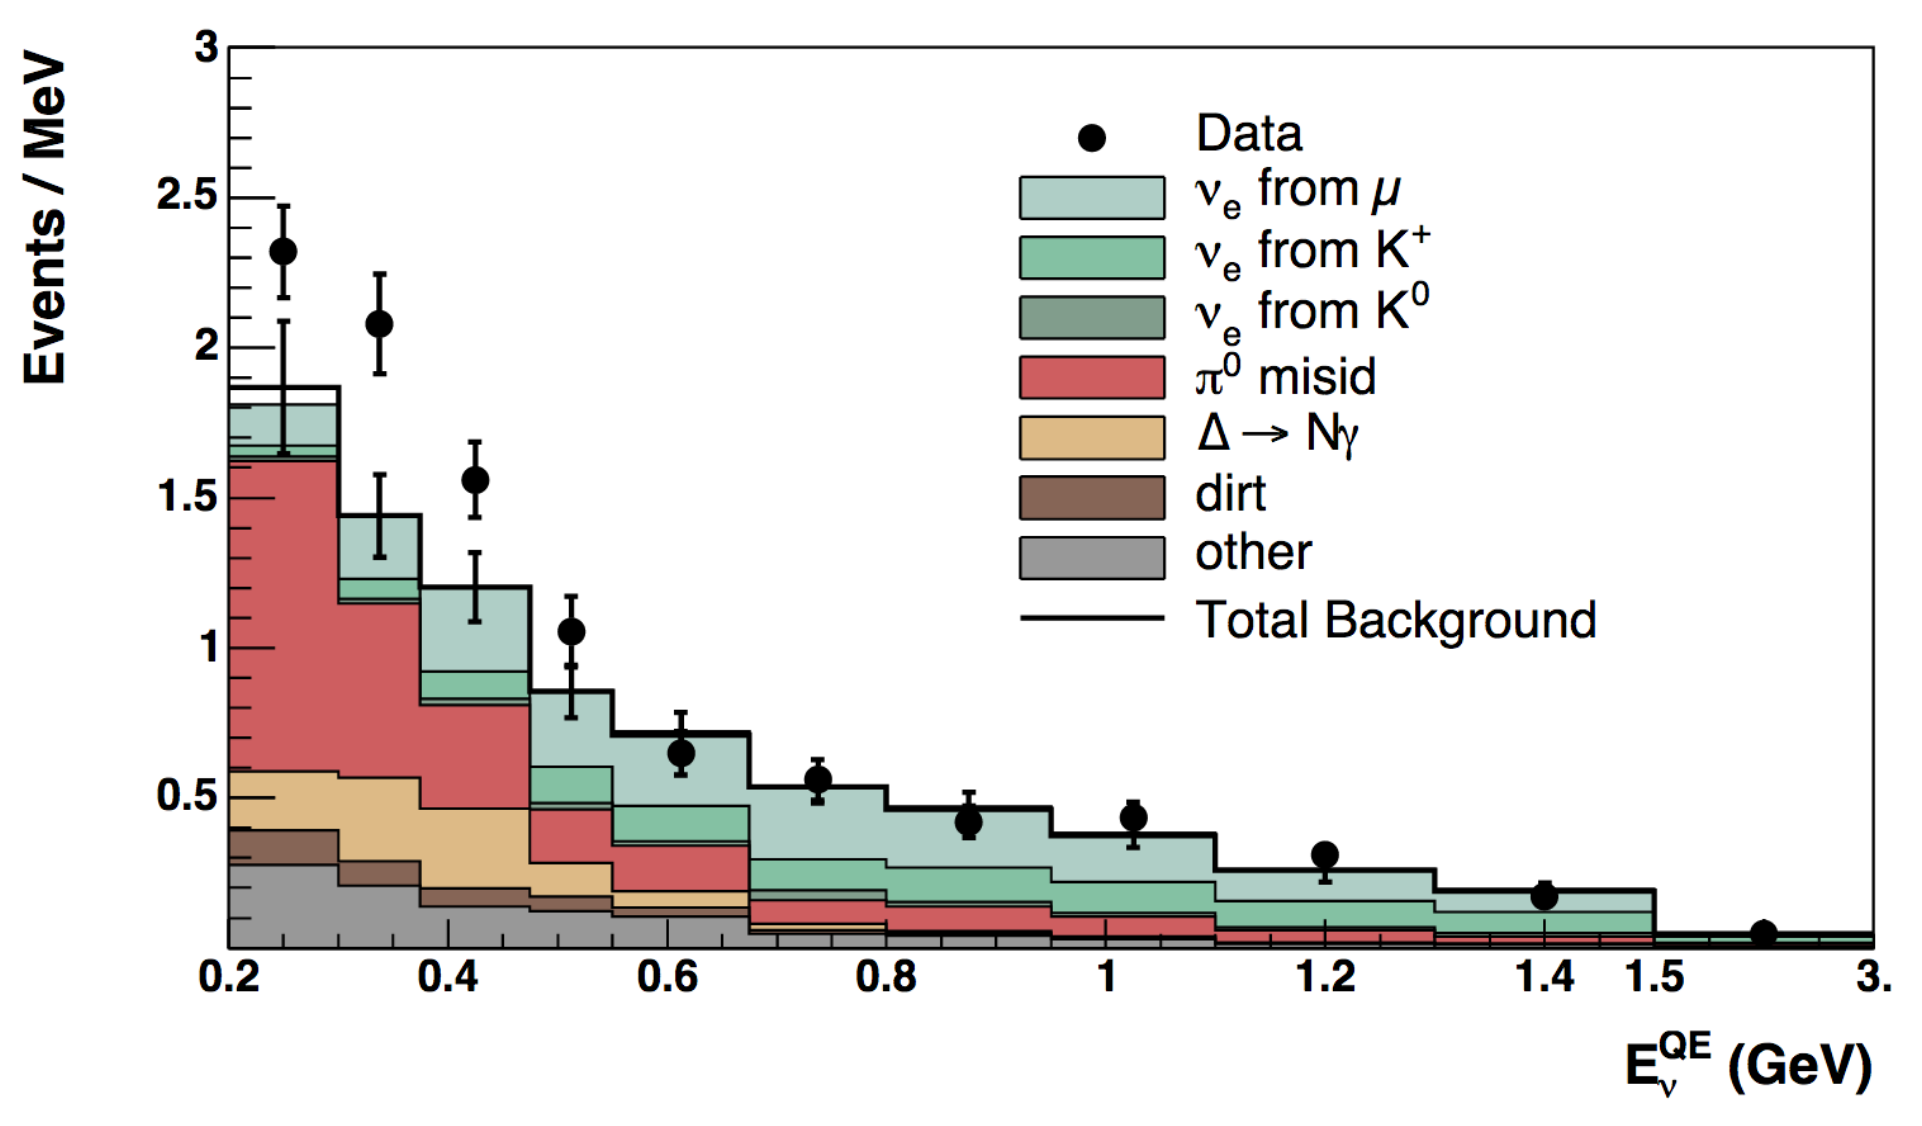
\includegraphics[width=0.9\textwidth]{Figures/MB_published_stackedhisto.png} \\
\caption{\textit{The $E_\nu^{QE}$ distribution for MiniBooNE data (points with statistical errors) and and backgrounds (histogram with systematic errors).}}\label{MB_published_stackedhisto_fig}
\end{figure}

\subsubsection{Proposed Low Energy Excess Sources}
% The LEE could either be electron like or photon like, MiniBooNE couldn't tell. Mention of theories like sterile neutrinos though no models seem to fit very well (3+1 or 3+2 with possible CP violation), single photon background misestimations or unexpected backgrounds, neutrino decay, lorentz violation etc etc. 
Shown in Figure \ref{MB_published_excess_fits_fig} is the MiniBooNE neutrino mode excess (data - expected background) with oscillation fits with parameters constrained to be in the LSND allowed region. The parameters in the LSND allowed region are ruled out at the 95\% confidence level if the data are fit with $E_\nu^{CCQE}$ > 475 MeV. \\

\begin{figure}[ht!]
\centering
	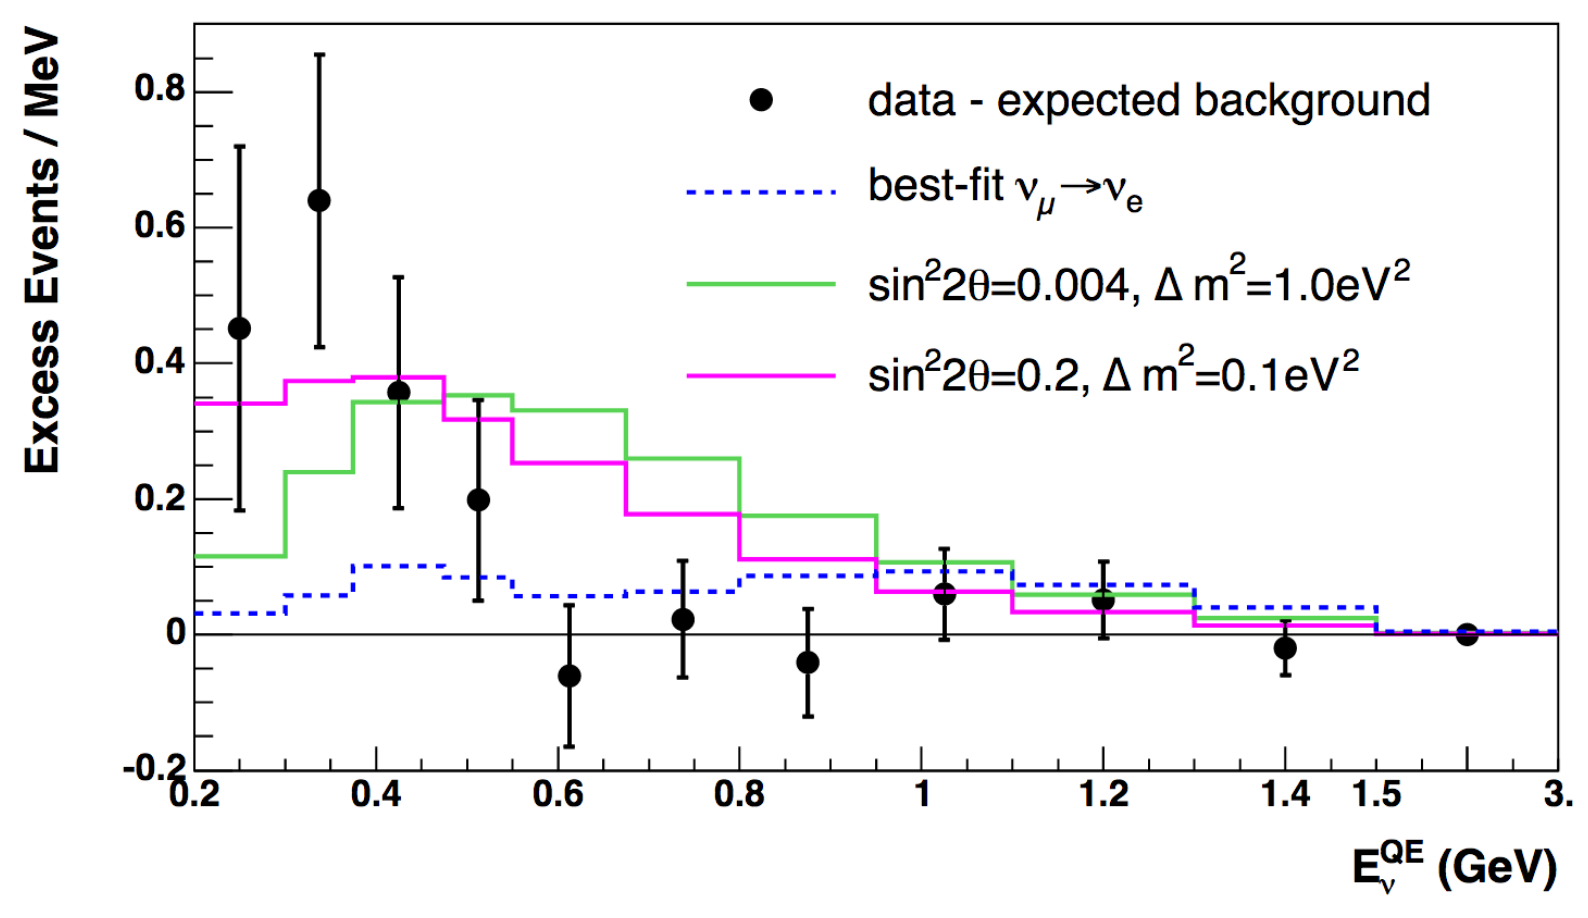
\includegraphics[width=0.9\textwidth]{Figures/MB_published_excess_fits.png} \\
\caption{\textit{The MiniBooNE event excess as a function of $E_\nu^{QE}$. Also shown are the expectations from the best oscillation fit and from neutrino oscillation parameters in the LSND allowed region. The error bars include both statistical and systematic errors.}}\label{MB_published_excess_fits_fig}
\end{figure}

Given MiniBooNE's inability to distinguish electrons from photons, the origin of this excess is either a mis-estimation of one of the backgrounds, or some sort of new physics. The former is unlikely the case because MiniBooNE makes many \textit{in situ} measurements that allow for the constraining of these backgrounds. The neutral current induced backgrounds (NC $\pi^0$, $\Delta\rightarrow N\gamma$, and dirt) are constrained by such measurements.\\

The NC $\pi^0$ rate in MiniBooNE is measured by selecting events with reconstructed mass near the $\pi^0$ mass and obtains a $>90$\% pure sample of NC $\pi^0$ interactions which is compared to simulation to obtain a correction function in order to bring the simulated distribution in agreement with data. This same correction function is applied to NC $\pi^0$ events that are backgrounds in the $\nu_e$ appearance analysis. This correction function increases the NC $\pi^0$ background by less than 13\% for $E_\nu^{CCQE}$ $<$ 400 MeV and decreases the background by as much as 20\% above this neutrino energy region. Including this correction factor, the uncertainty on the overall NC $\pi^0$ backgrounds is 7\%. Note that a correction factor of 2.0 would be required to explain the origin of the excess as originating from a misestimated NC $\pi^0$ background.(XXX citation here... got this from Georgia's thesis)\\

The excess is unlikely caused by a misestimation of the $\Delta\rightarrow N\gamma$ backgrounds because they are additionally constrained by the NC $\pi^0$ measurement through the relative rate of resonant production times a branching fraction of (0.56$\pm$0.04)\% (XXX citation here... got this from Georgia's thesis). With this measurement, the uncertainty on the $\Delta\rightarrow N\gamma$ backgrounds is 12\%. Note that a correction factor of 2.7 would be required to explain the origin of the excess as originating from a misestimated $\Delta \rightarrow N\gamma$ background.\\

The excess is unlikely caused by a misestimation of the dirt backgrounds because a direct measurement is made by selecting a separate event sample which are likely dirt events and comparing data to simulation. These events are reconstructed close to the detector boundaries with direction pointed generally inwards. In neutrino mode, a dirt background normalization correction factor was computed to be 0.7 $\pm$ 0.1 (with simulation over-predicting the dirt rate normalization). Given the power of the event selection cuts designed to mitigate dirt backgrounds, the relevance of this relatively large correction factor is minimal.\\

The charged current induced backgrounds (intrinsic $\nu_e$CCQE) are reduced with \textit{in situ} measurements of $\nu_\mu$CCQE interactions. A data to simulation comparison of measured $\nu_\mu$CCQE interactions allows for the retuning of underlying flux and cross section parameters in order to bring simulated distributions in agreement with data. These parameters are the same as those used to predict the $\nu_e$CCQE rate and shape. In addition, a measurement of the highest energy $\nu_\mu$CCQE interactions allows for the further constraint of $\nu_e$CCQE from kaon decay backgrounds, which is discussed in more detail in a later section of this thesis.\\

Given the likelihood that the excess is not caused by misidentified backgrounds, several new-physics interpretations have been proposed in attempt to explain the excess, including sterile neutrino oscillations (with one, two, or more sterile neutrinos), and new interactions both within and outside of the standard model (CPT violation, quantum decoherence, sterile neutrino decay, etc). A summary of these interpretations can be found in \cite{MBLEESourcesOverview}. A commonality between all interpretations is that their interactions pass the MiniBooNE event selection cuts; that is, they have one electron or one photon exiting the interaction vertex.

\subsection{MicroBooNE In The Context of the Low Energy Excess}
% Discussion of how as a LArTPC MicroBooNE has electron/photon separation. Showing the scaled signal plot from the TDR. Mention that this scaled signal is oversimplified so that's why this thesis describes a more rigorous sensitivity study with simulation in MicroBooNE.

%http://microboone-docdb.fnal.gov:8080/cgi-bin/RetrieveFile?docid=3528&filename=low-E-excess-note.pdf&version=2
Given the proposed explanations for the origin of the measured MiniBooNE low energy excess in neutrino mode all predict either a single electron or single photon produced at the neutrino interaction vertex, and that MiniBooNE cannot discriminate between single electrons or photons, the MicroBooNE experiment was proposed. This detector (described in detail in Section \ref{XXXMICROBOONEDETECTORSECTIONXXX}) is a liquid argon time projection chamber, a relatively new detector technology which allows for the discrimination between single electrons and photons based on the energy deposition at the start of their tracks (photons will pair produce and in general have twice the ionization as a single electron). MicroBooNE runs in the same beam line (BNB) in neutrino mode and is physically located very close to MiniBooNE. Therefore, MicroBooNE should be able to elucidate the MiniBooNE low energy excess ambiguity. \\

A preliminary attempt to scale the MiniBooNE backgrounds and excess to the MicroBooNE both under the assumption that the excess is due to an electron-like event (left) or under a photon-like event (right) \cite{UBTDR} is shown in Figure \ref{TDR_LEE_scaling_fig}. The resulting statistical significance after the nominal amount of data is taken in MicroBooNE ($6.6\times 10^20$ POT) is computed to be 5.7$\sigma$ under the single-electron excess hypothesis and 4.1$\sigma$ under the single-photon hypothesis. Note that this scaling is assuming the electron/photon misidentification rate in MicroBooNE is assumed to be 6\% (whereas it is 100\% for MiniBooNE). Also event selection efficiencies in MicroBooNE are assumed to be twice that of MiniBooNE because of the detector technology. This scaling procedure also ignores other potentially important differences between MicroBooNE and MiniBooNE including differences in detector geometry (important for $\pi^0$ misidentifications in which one photon escapes), flux differences (which are non-negligible despite the relative close physical proximity of the two detectors), event topology selection differences (MicroBooNE can see much more vertex activity than can MiniBooNE, especially when additional final state particles are below Cherenkov threshold), the differing cosmic rejection background efficiencies (MiniBooNE can reject cosmics much more efficiently than MicroBooNE), cross section differences between argon and $CH_2$ arising from differing proton to neutron ratios, among other things.\\

\begin{figure}[ht!]
\centering
	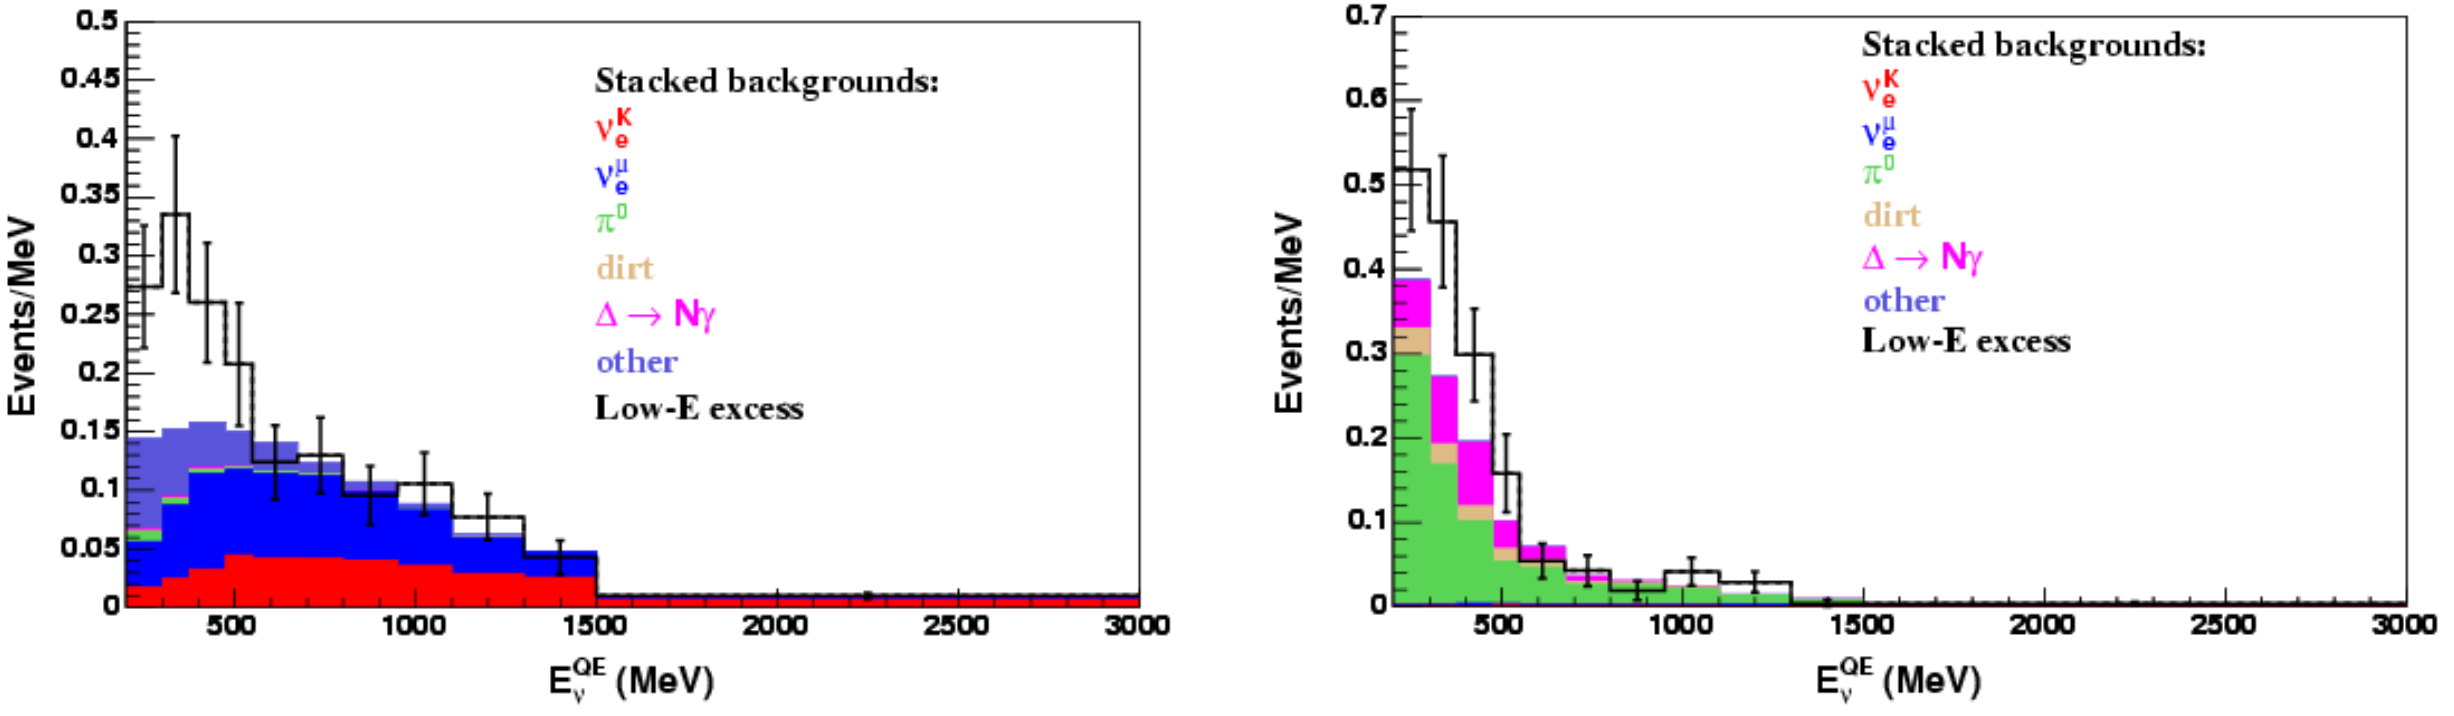
\includegraphics[width=0.9\textwidth]{Figures/TDR_LEE_scaling.png} \\
\caption{\textit{A preliminary attempt to scale the MiniBooNE backgrounds and excess to the MicroBooNE both under the assumption that the excess is due to an electron-like event (left) or under a photon-like event (right). Stacked histograms show the expected background. Error bars indicate statistical uncertainty. The number of signal events, scaled from MiniBooNE for neutrino flux and fiducial volume, is the same in both plots. Both plots assume $6.6 \times 10^20$ POT for the MicroBooNE 60 ton fiducial mass.}}\label{TDR_LEE_scaling_fig}
\end{figure}

While the aforementioned scaling of MiniBooNE backgrounds to MicroBooNE provides a reasonable estimate of the expected sensitivity to the MiniBooNE low energy excess, it is oversimplified for the reasons mentioned. The next sections in this thesis describe a more rigorous analysis with the ultimate goal of computing MicroBooNE's sensitivity to the MiniBooNE low energy excess assuming the single-electron hypothesis. In this analysis, signal and background events will be simulated in the MicroBooNE detector and event selection cuts and algorithms will be used to select the events














\section{Monte Carlo Simulation}

\subsection{Simulated Background Samples}\label{LEE_simulated_background_samples_section}
In this analysis, both beam induced backgrounds and beam external backgrounds are simulated in the MicroBooNE cryostat. For beam-induced samples, the same flux predictions are used as were used in the MiniBooNE simulations (accounting for baseline and acceptance differences). The beam-induced samples come from full simulated BNB interactions with cross sections provided by GENIE (XXX citation). Beam-external samples (cosmics) come from simulated CORSIKA generated (XXX citation) cosmic rays that pass through the cryostat. Cosmic rays passing through other portions of the detector hall but not the cryostat result in negligible backgrounds in this $\nu_e$ search. The passage of all particles through the detector volume is simulated by the {\sc GEANT4} package (XXX citation). XXX here is where i can mention that GENIE generates the neutrino interactions in UB but NUANCE does in MB, then use NUISANCE to compare the two.

\subsection{Reconstruction}
Ideally this analysis would be done on fully automated reconstructed objects. Such objects would be created from only the output wire and PMT signals from the detector. In this way, the same reconstruction methods could be used on data as are used in simulation. Unfortunately, at the time this thesis was written, the automated reconstruction in MicroBooNE is not adequate to do any sort of sensitivity study.\\

In general, the output of an automated reconstruction chain in a LArTPC consists of reconstructed optical hits which come from the PMT signals, and reconstructed wire hits which come from drift electron ionization signals on the induction and collection plane wires. Reconstruction algorithms cluster the latter hits on each wire plane into those corresponding ot individual particles, then match clusters from different wire planes to form 3D reconstructed objects. The wire planes provide two of the three dimensions, and matching clusters to optical hits on the PMTs provide the third (drift) dimension. These reconstructed objects are either thin, straight tracks (which come from particles like muons, charged pions, and protons) or more fuzzy showers, which come from higher energy electrons or photons. While automatic track reconstruction can currently be performed at an adequate level, the difficulties involved in shower reconstruction (which is particularly important to tag and study $\nu_e$CC events) have yet to be overcome.\\

For these reasons, this simulation-only study is done with objects that are not automatically reconstructed from wire and PMT signals, but instead from truth-based energy depositions in the detector. In general, these objects represent what would be reconstructed from wire and PMT signals if the reconstruction algorithms performed perfectly. Therefore, this is referred to as ``perfect reconstruction'' and the details of it are discussed in the next section. 

\subsubsection{``Perfect Reconstruction''}\label{perfectreco_section}
% Description of what {\sc MCTracks} and {\sc MCShowers} are, how they're made, etc. Make it clear that they are the input to the event reconstruction algorithms. Also make it clear that this entire sensitivity study is done only with these objects; no real automated reconstruction is covered (which is why no results on data are shown).
While a simulation-only study using real automated reconstruction would be ideal, such a study using ``perfect reconstruction'' is incredibly valuable; it is a step forward from the aforementioned simple scaling study, and the event selection cuts and algoritihms designed in this study can be used out-of-the-box on automated reconstructed objects once they become available. Additionally, the ``perfect reconstruction'' can be tuned to more realistically represent what automated reconstruction might be capable of, for example by smearing the energy of objects or emulating realistic reconstruction efficiencies. This will provide the important estimate of systematic uncertainties arising from automated reconstruction.\\

As mentioned earlier, the final 3D reconstructed objects formed from wire plane signals and PMT signals are referred to as tracks or showers. Tracks are close to straight lines in three dimensions, while showers are fuzzier and generally cone-shaped in three dimensions. The ``perfect reconstruction'' analogs to tracks and showers are referred to as {\sc MCTracks} and {\sc MCShowers}. They are created from simulated {\sc GEANT4} 3D energy depositions in the detector volume. {\sc GEANT4} outputs 3D energy depositions in the detector, along with truth information about which parent particles deposited this energy. {\sc MCShowers} and {\sc MCTracks} are 3D objects which are formed by grouping energy depositions based on parent particles. Whether a particle in {\sc GEANT4} becomes an {\sc MCShower} or an {\sc MCTrack} is based on truth PDG (for example, electrons always form {\sc MCShower}s and muons always form {\sc MCTrack}s). Only the energy deposited by particles \textit{within the TPC} is used to form these ``perfect reconstructed'' objects, which is in line with them representing actual reconstructable quantities (no ionization outside of the TPC is reconstructable).\\

To clarify, consider the following simulated interaction: a $\nu_e$ charged current interaction in which the final state particles are an electron, a charged pion, a neutral pion, and two protons. The charged pion travels until it stops, where it decays into a muon, which then travels and decays into an electron. The generated ``perfect reconstruction'' objects in the event will be four {\sc MCTracks} (for the electron exiting the interaction, the electron from the muon decay, and one for each photon originating from the neutral pion decay) and four {\sc MCTracks} (one for the charged pion, one for the muon, and one for each proton).\\

{\sc MCTracks} consist of a series of ordered 3D trajectory points, each corresponding to an energy deposition in the detector. {\sc MCShowers} have the following attributes: 3D start point where the first energy from the parent particle is deposited, 3D direction which is computed by fitting a line in 3D to all of the deposited energy from the parent particle, and dE/dx computed from the energy depositions along the first few centimeters of the shower. These ``perfectly reconstructed'' tracks and showers ({\sc MCTracks} and {\sc MCShowers}) serve as the input to the event selection algorithms, just as automated reconstructed tracks and showers would be in real data.\\




\section{Event Selection}
This section describes the algorithms and cuts used to identify $\nu_e^{CCQE}$ interactions, given as input the ``perfect reconstructed'' {\sc MCTracks} and {\sc MCShowers} from simulated triggered events in MicroBooNE\footnote{Note that these cuts and algorithms could use automatically reconstructed tracks and showers, and therefore could be run both on simulation and data, if the quality of track and shower reconstruction was high enough.}. With these reconstructed objects in hand, a series of nine algoritihms are run, each with a specific goal in mind; they either identify background topologies in order to remove them, or they identify the signal topology. For example, one algorithm identifies {\sc MCShowers} which are likely delta rays originating from tracks. Once identified, these {\sc MCShowers} are no longer candidate $\nu_e^{CCQE}$ electrons. Another algorithm looks for pairs of showers that are likely from $\pi^0$ decays in order to remove them from the pool of candidate $\nu_e^{CCQE}$ electrons. Another algorithm looks for through-going tracks to tag them as cosmic, ensuring they will not be associated with a neutrino interaction. The two most important event selection algorithms for this analysis are named ``AlgoEMPart'' (which handles the electron/photon discrimination based on {\sc MCShower} deposited energy near its start point) and ``AlgoSingleE'' (which is the algorithm responsible for locating the $\nu_e^{CCQE}$ topology and associating all {\sc MCTracks} and {\sc MCShowers} together for eventual energy reconstruction and analysis). These two algorithms are discussed in detail in the following two subsections. The remaining seven event reconstruction algorithms are discussed in detail in the appendices of this thesis.

% This section describes how we take reconstructed objects (tracks and showers) and identify nue interactions. Mention that the analysis framework has many algorithms that each serve a specific purpose. Briefly mention the algorithms by name and what they're intended to do. Include the flowchart figure from the APS technote listing all the algorithms and the order in which they are executed. The following sections will describe in more detail the important ones. 

\subsection{Electron/Photon Separation Algorithm}\label{algoempart_section}
% This is the algorithm (AlgoEMPart) that uses the reconstructed dE/dx and conversion distance to form a likelihood that a shower is electron like or photon like. It's one of the most important and should be described in detail. Include some figures showing performance of this algorithm.
The way electron/photon separation based on dE/dx at the start of showers is with an algorithm called ``AlgoEMPart". This algorithm uses trained likelihood distributions which input dE/dx and return the likelihood that the shower is electron-like, or photon-like. If a conversion distance is known, it will incorporate that into its likelihood as well. The likelihood is configured with parameters output by a RooFit minimization routine. The RooFit routine is trained on simulated single electron and single photon {\sc MCShowers}. In general, this algorithm computes both the likelihood that an {\sc MCShower} is an electron and that it is a photon, and determines the identity of the particle to be the one with the larger likelihood.\\

There are two likelihood functions that may be used. If an {\sc MCShower} can independently be associated with a neutrino interaction vertex, AlgoEMPart will use a 2D likelihood function that includes both dE/dx and radiation length information. If an algorithm cannot associate a vertex with a shower, there is a 1D likelihood function that can be used with only dE/dx information. The 1D likelihood function is composed of a gaussian plus a landau distribution for dE/dx, and the 2D likelihood function also includes an exponential function for radiation length. Any potential energy dependence on dE/dx or conversion distance is not included in these likelihoods. The twelve trained input parameters include mean and sigma values for the gaussian distributions, the MPV and sigma values for the landau distributions, the fractional area difference between the gaussian and landau distributions, and the radiation length parameter (six parameters for electrons, six parameters for photons). When training, input parameters for each sample (electron, photon) are the {\sc MCShower} computed dE/dx as well as the truth-level creation vertex of the particle.

\subsubsection{Performance}\label{empart_perfectreco_performance}
The performance of this algorithm on ``perfect reconstruction" is computed by using samples of single electron showers and single photon showers generated isotropically between 0.05 and 2 GeV, and selecting those events where greater than 90\% of the shower's energy is contained within the TPC. The algorithm's likelihood is trained using this sample (integrated over the full energy range of the showers). 
\begin{enumerate}
\item Using \textit{only dE/dx} information, the efficiency (over all energies) to select a single electron is 93\%, while the MID efficiency to tag the electron as a photon is 7\%. 
\item Using \textit{only dE/dx} information, the efficiency to select a single photon is 97.3\%, while the MID efficiency to tag the photon as an electron is 2.7\%.
\item Using \textit{both dE/dx and radiation length} information (using the true creation point of photons), the efficiency to select a single electron is 99.7\%, while the MID efficiency to tag the electron as a photon is 0.3\%. 
\item Using \textit{both dE/dx and radiation length} information (using the true creation point of photons), the efficiency to select a single photon is 98.1\%, while the MID efficiency to tag the photon as an electron is 1.9\%.
\end{enumerate}


The 1D likelihood to determine if a shower is electron-like or photon-like is shown in Figure \ref{empart_perfectreco_performance_fig4}. The likelihood that a shower with a given dE/dx is electron-like is computed by the ratio of the 1D electron-like PDF value for that dE/dx (shown non-normalized in Figure \ref{empart_perfectreco_performance_fig2}) to the sum of the electron-like PDF value for that dE/dx and the photon-like PDF value for that dE/dx (shown non-normalized in Figure \ref{empart_perfectreco_performance_fig2} as well) (Equation \ref{1D_dedx_likelihood_eqtn}). 

\begin{equation}\label{1D_dedx_likelihood_eqtn}
LL_e=\frac{e_{dE/dx}^{PDF}(\frac{dE}{dx})}{ e_{dE/dx}^{PDF}(\frac{dE}{dx}) + g_{dE/dx}^{PDF}(\frac{dE}{dx}) }
\end{equation}
where $e_{dE/dx}^{PDF}(\frac{dE}{dx})$ represents the electron dE/dx PDF function (shown non-normalized in Figure \ref{empart_perfectreco_performance_fig2}) evaluated at a dE/dx value $\frac{dE}{dx}$ and $g_{dE/dx}^{PDF}(\frac{dE}{dx})$ represents the photon dE/dx PDF function (also shown non-normalized in Figure \ref{empart_perfectreco_performance_fig2}) evaluated at a dE/dx value $\frac{dE}{dx}$. The likelihood that a shower with a given dE/dx is photon-like is similarly computed but with the photon-like PDF value for that dE/dx in the numerator.\\

The 2D likelihood including both dE/dx and conversion distance is shown in Figure \ref{empart_perfectreco_performance_fig1}. The likelihood that a shower with a given dE/dx value, $\frac{dE}{dx}$ and a given conversion distance value, $d$ is electron-like is computed as follows: 
\begin{equation}\label{2D_likelihood_eqtn}
LL_e=log( \frac{e_{dE/dx}^{PDF}(\frac{dE}{dx}) * e_{conv}^{PDF}(d)}{g_{dE/dx}^{PDF}(\frac{dE}{dx}) * g_{conv}^{PDF}(d)} )
\end{equation}
where $e_{dE/dx}^{PDF}(\frac{dE}{dx})$ represents the electron dE/dx PDF function (shown non-normalized in Figure \ref{empart_perfectreco_performance_fig2}) evaluated at a dE/dx value, $\frac{dE}{dx}$, $e_{conv}^{PDF}(d)$ represents the electron conversion distance PDF function (shown non-normalized in Figure \ref{empart_perfectreco_performance_fig6}) evaluated at a conversion distance value, $d$, $g_{dE/dx}^{PDF}(\frac{dE}{dx})$ represents the photon dE/dx PDF function (shown non-normalized in Figure \ref{empart_perfectreco_performance_fig3}) evaluated at a dE/dx value, $\frac{dE}{dx}$, $g_{conv}^{PDF}(d)$ represents the photon conversion distance PDF function (shown non-normalized in Figure \ref{empart_perfectreco_performance_fig7}) evaluated at a conversion distance value, $d$. The likelihood that the same shower is photon-like is simply the inverse of Equation \ref{2D_likelihood_eqtn}.\\


\begin{figure}[ht!]
\centering
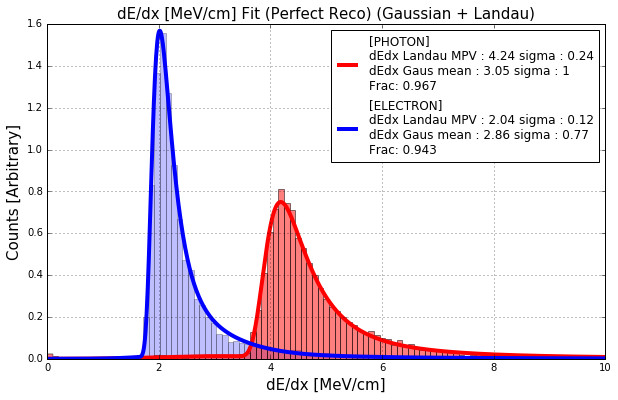
\includegraphics[width=100mm]{Figures/EMPartTraining/mc_trained/dEdx_Selected_both.png}\\
\caption{\textit{AlgoEMPart training results on perfect reconstructed electron showers and on perfect reconstructed photon showers as described in Section \ref{empart_perfectreco_performance}: 1D landau + gaussian fit to dE/dx.}}
\label{empart_perfectreco_performance_fig2}
\end{figure}

\begin{figure}[ht!]
\centering
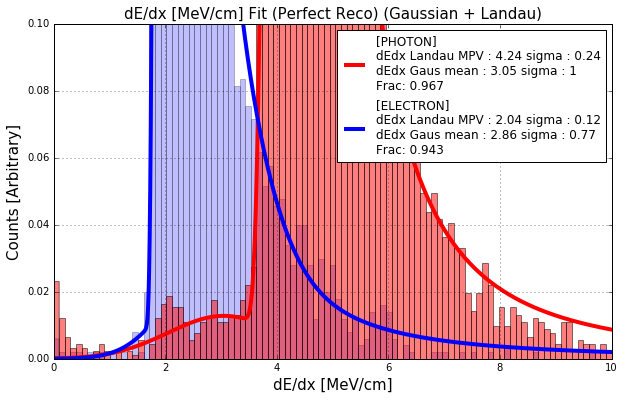
\includegraphics[width=100mm]{Figures/EMPartTraining/mc_trained/dEdx_Selected_both_zoomed.png}\\
\caption{\textit{The same plot as shown in Figure \ref{empart_perfectreco_performance_fig2}, but zoomed in along the y-axis to show the compton peak in the photon sample, as well as the pileup of very low dE/dx values for photons (due to soft compton scatters as described in Section \ref{perfectreco_section}).}}
\label{empart_perfectreco_performance_fig3}
\end{figure}

\begin{figure}[ht!]
\centering
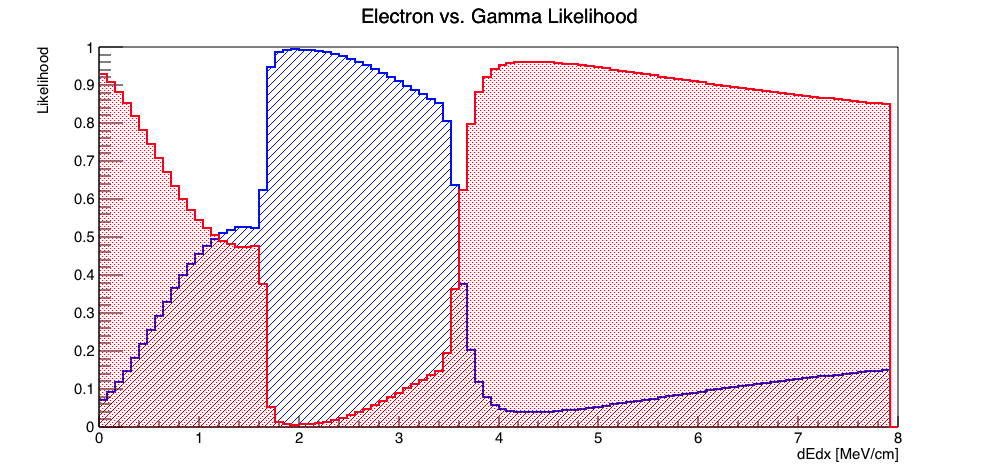
\includegraphics[width=100mm]{Figures/EMPartTraining/mc_trained/Likelihood_dEdx.png}\\
\caption{\textit{AlgoEMPart: Computed 1D likelihood vs dE/dx: red is photon, blue is electron. How the likelihood is computed is described in Section \ref{empart_perfectreco_performance}.}}
\label{empart_perfectreco_performance_fig4}
\end{figure}


\begin{figure}[ht!]
\centering
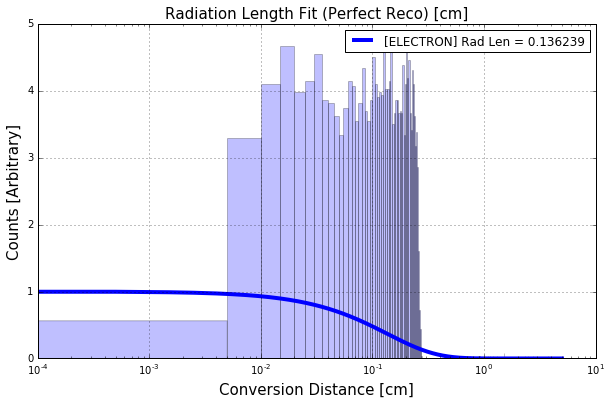
\includegraphics[width=100mm]{Figures/EMPartTraining/mc_trained/RadLength_Selected_e.png}\\
\caption{\textit{AlgoEMPart training results on perfect reconstructed electron showers as described in Section \ref{empart_perfectreco_performance}: Radiation length fit to single electron showers. Note the poor quality of the fit as the electron conversion distance for ``perfect reconstruction'' does not follow an exponential distribution; all conversion distances are below 0.3 centimeters.}}
\label{empart_perfectreco_performance_fig6}
\end{figure}

\begin{figure}[ht!]
\centering
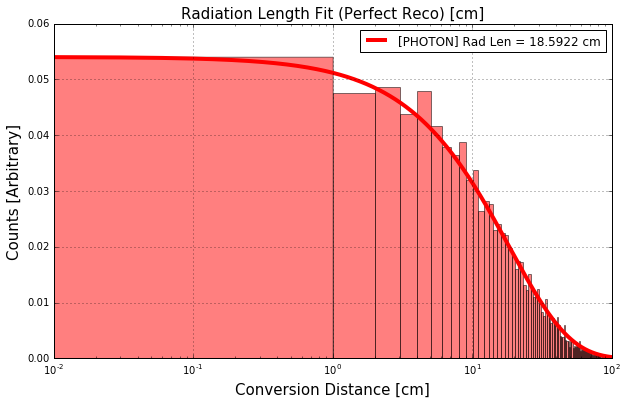
\includegraphics[width=100mm]{Figures/EMPartTraining/mc_trained/RadLength_Selected_g.png}\\
\caption{\textit{AlgoEMPart training results on perfect reconstructed photon showers as described in Section \ref{empart_perfectreco_performance}: Radiation length fit to single photon showers.}}
\label{empart_perfectreco_performance_fig7}
\end{figure}


\begin{figure}[ht!]
\centering
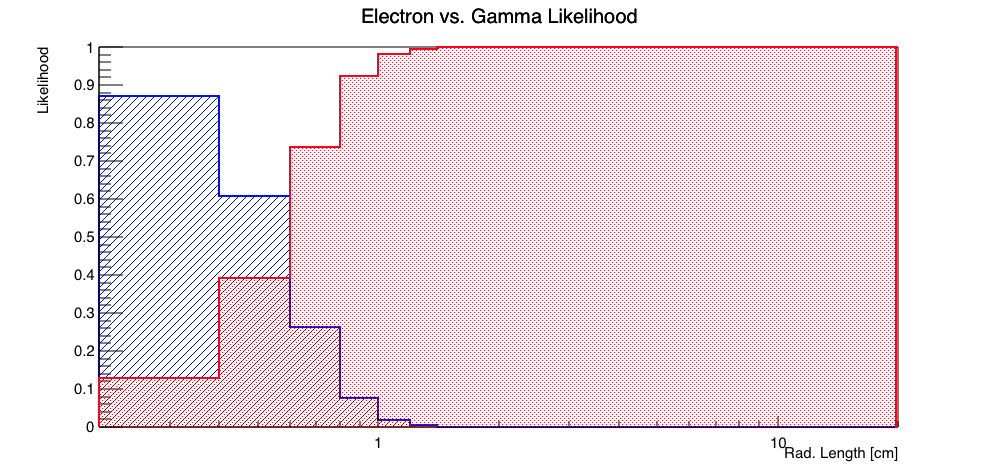
\includegraphics[width=100mm]{Figures/EMPartTraining/mc_trained/Likelihood_radLen.png}\\
\caption{\textit{AlgoEMPart: Computed 1D likelihood vs conversion distance (integrated over all energies): red is photon, blue is electron. How the likelihood is computed is described in Section \ref{empart_perfectreco_performance}.}}
\label{empart_perfectreco_performance_fig5}
\end{figure}

\begin{figure}[ht!]
\centering
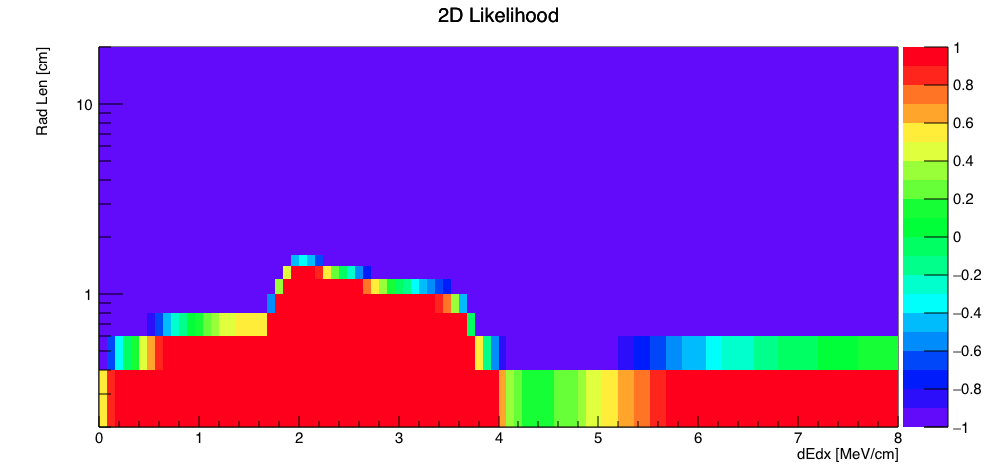
\includegraphics[width=100mm]{Figures/EMPartTraining/mc_trained/2DRatio.png}\\
\caption{\textit{AlgoEMPart training results on perfect reconstructed electron and photon showers as described in Section \ref{empart_perfectreco_performance} integrated over all energies: 2D likelihood distribution (radiation length vs. dE/dx). Low values of likelihood (purple) correspond to photon-like, high values (red) correspond to electron-like.}}
\label{empart_perfectreco_performance_fig1}
\end{figure}























































\subsection{Signal Selection Algorithm}

The purpose of this algorithm is to reconstruct events with $\nu_e$CC inclusive type topologies. These topologies involve a single electron at a neutrino interaction vertex, with any number of protons, charged or neutral pions, or anything else additionally exiting the vertex. Later on, the sample of selected events will be subjected to further cuts to select only $\nu_e$CCQE topologies by rejecting events with pions in the final state. This algorithm uses likelihoods provided by AlgoEMPart (Section \ref{algoempart_section}) to determine if a shower is an electron or a photon. This algorithm begins by looping over all candidate $\nu_e$CC electron showers in the event that have not been removed by upstream cosmic and $\pi^0$ tagging algorithms. Figure \ref{algosinglee_flowchart_fig} is a flowchart depicting decisions the algortihm makes for each candidate $\nu_e$CC electron shower. If the algorithm gets to the bottom of the flowchart, that shower was determined to be from a $\nu_e$CC interaction and the event is saved to be included in analysis. The flowchart refers to determining if two showers are correlated and determining if a shower is correlated with the start of a track. A schematic which diagrams how these determinations are made is shown in Figure \ref{algosinglee_cartoon_fig}. A list of configurable parameters and their chosen cut values can be found in Table \ref{algosinglee_table}.\\


\begin{figure}[ht!]
\centering
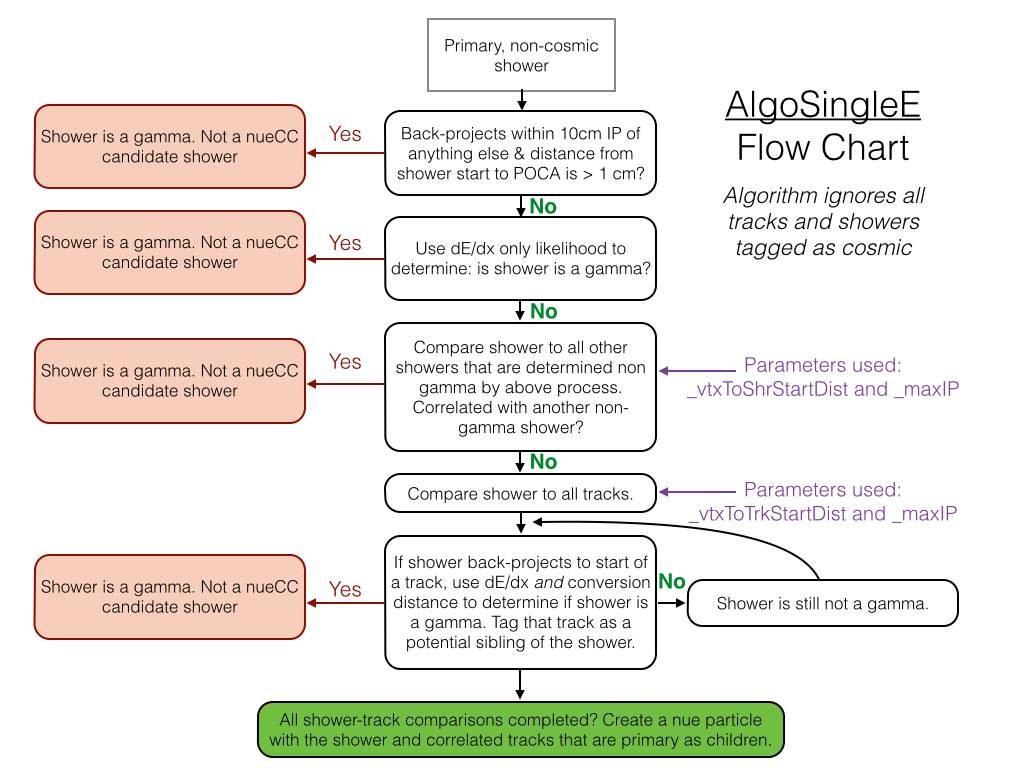
\includegraphics[width=150mm]{Figures/algosinglee_flowchart.png}\\
\caption{\textit{A flowchart depicting decisions the algortihm makes for each primary, non-cosmic shower. If the algorithm gets to the bottom of the flowchart, that shower was determined to be from a $\nu_e$CC interaction, and a $\nu_e$ particle is created.}}
\label{algosinglee_flowchart_fig}
\end{figure}

\begin{figure}[ht!]
\centering
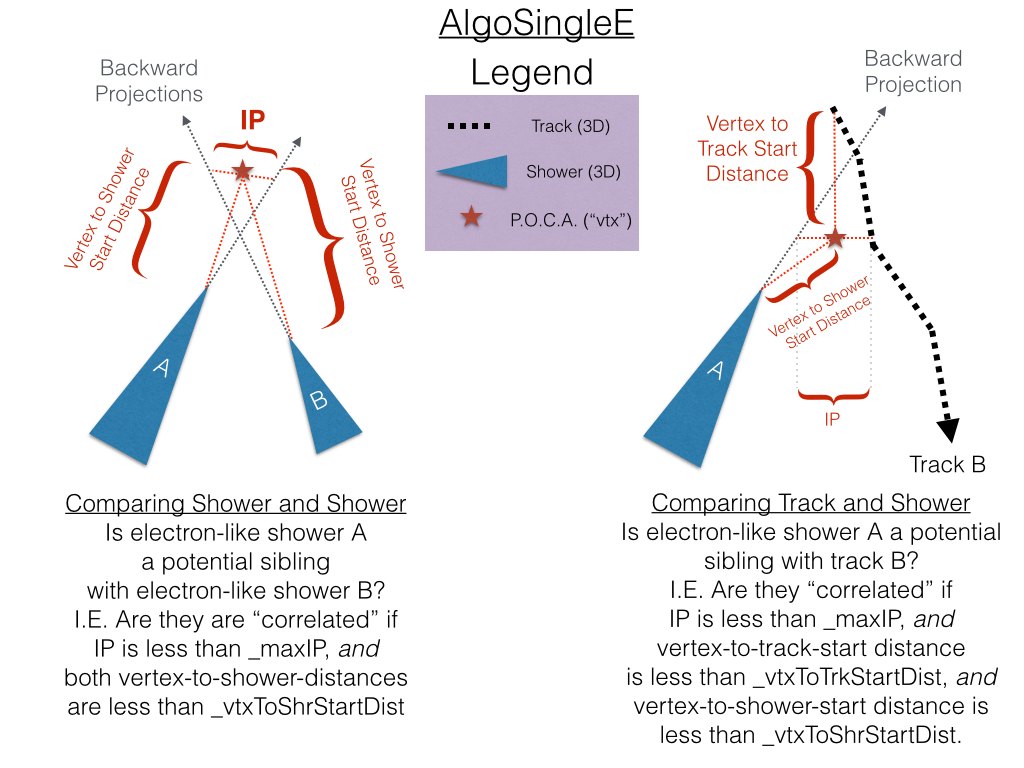
\includegraphics[width=150mm]{Figures/algosinglee_cartoon.png}\\
\caption{\textit{Schematic cartoons indicating how the signal selection algorithm makes decisions determining if two reconstructed showers are correlated, and if a reconstructed shower is correlated with a reconstructed track (as described in Figure \ref{algosinglee_flowchart_fig}).}}
\label{algosinglee_cartoon_fig}
\end{figure}

A more detailed description of Figure \ref{algosinglee_flowchart_fig} is given in the following paragraphs.\\

For each primary, non-cosmic shower (``shower A''), this algorithm computes the point of closest approach and impact parameter between the shower's back-projection and to all other tracks, as well as to all other shower back-projections (see Figure \ref{algosinglee_cartoon_fig} ). If the smallest impact parameter (IP) is less than 10 centimeters and the distance between the shower's start point and the point of closest approach (Vertex-to-Shower-Start-Distance) is greater than 1 centimeter, the algorithm assumes this shower is a photon and it rejects the shower as a potential $\nu_e$CC shower, without any dE/dx considerations. Otherwise, the algorithm continues by using AlgoEMPart's trained likelihood function to determine based on dE/dx alone whether this shower is gammalike and should therefore be ignored.\\

Assuming this potential $\nu_e$CC shower (``shower A'') has so far been found to be electron-like, the algorithm then compares the shower to all other showers in the event that are not marked as cosmic, and are not already reconstructed to be the descendant of another particle. The purpose of this portion of the code is to enforce that the topology of interest includes a \textit{single electron} exiting the neutrino interaction. If any other electron-like showers are nearby (with Vertex-To-Shower-Start-Distance less than \_vtxToShrStartDist and IP less than \_maxIP) that could be potentially correlated, ``shower A'' is rejected as a candidate $\nu_e$CC electron.\\

Assuming ``shower A'' has not yet been rejected, it is then compared to every non-cosmic track in the event that has not been tagged as cosmic and is longer than 0.3cm (a value chosen because it is the wire spacing and tracks shorter than one wire spacing are assumed non reconstructable). The purpose of this portion of the code is to look for correlations between the potential $\nu_e$CC electron and tracks (Figure \ref{algosinglee_cartoon_fig}). The topology of interest allows for the electron to point back to the \textit{start} of a track, but \textit{not} to the middle or end of a track (as these showers are likely delta rays or Michel electrons). For each ``shower A''-to-track comparison, the point of closest approach (P.O.C.A.) between the shower's backward projection and the track's trajectory is computed. If the impact parameter between the shower and the track is less than a configurable distance (\_maxIP) and the distance between the start point of the track and the P.O.C.A. is less than a configurable distance (\_vtxToTrkStartDist) and the distance between the start point of the shower and the P.O.C.A. is less than a configurable distance (\_vtxToShrStartDist) then there is a potential acceptable correlation between ``shower A'' and the start of the track. At this point, the code again uses a likelihood from AlgoEMPart to determine if the shower is still electron-like, this time using both the shower's dE/dx \textit{and} the distance between the shower start and the computed P.O.C.A. as a radiation length. This is a more powerful discrimination to determine if the shower remains electron-like. If ``shower A'' remains electron-like and is found to be correlated with the start of a track, the track is marked to be added as a potential sibling of the shower if this shower is eventually found to be the child of a $\nu_e$CC interaction.\\

If ``shower A'' has not yet been rejected, a $\nu_e$CC event has been found. The algorithm creates a $\nu_e$ particle in the reconstructed particle graph with vertex at the electron shower's start point. It sets the parentage such that the electron and all associated tracks are children of the neutrino.

\subsubsection{Configurable Parameters}
The configurable parameters for this algorithm are summarized in the following table. Note that with ``perfect reconstructed'' showers, these distances are always very small (less than 0.1 centimeters), so these values were chosen to introduce some realism into the algorithm by estimating detector resolutions. They were chosen more loosely to include photons that had a short conversion distance.\\\\

\begin{center}
\begin{tabular}{ |p{8cm}|p{3.5cm}|p{1.5cm}|  }
 \hline
 \multicolumn{3}{|c|}{AlgoSingleE: Parameters} \\
 \hline
 Parameter Name & Code Variable & Cut Value \\
 \hline \hline
 Use Radiation Length & \_useRadLength & True\\\hline
 
 Max Vertex-to-Track-Start Distance & \_vtxToTrkStartDist & 1 cm \\\hline

 Min Vertex-to-Shower-Start Distance & \_vtxToShrStartDist & 50 cm \\\hline

 Maximum IP & \_maxIP & 1 cm \\\hline

 \hline
\end{tabular}\label{algosinglee_table}
\end{center}


\subsubsection{Performance}

XXX mention the efficiency to select signal, and the MID efficiencies to select backgrounds.
































\subsection{Energy Reconstruction}
%Description of the energy definition. Mention that it is different than the CCQE energy definition MiniBooNE used. Include a figure of Ereco vs Etrue for the intrisic nue sample.

With the candidate $\nu_e$CCQE interactions identified, the neutrino energy is reconstructed in two ways. First, the angle and energy of the selected $\nu_e$CCQE electron is used to compute an energy, $E_\nu^{CCQE}$ from the CCQE formula, Equation \ref{MB_CCQE_formula}. This is the same energy definition that is used in the MiniBooNE oscillation analysis.\\

An additional, more accurate energy estimation, $E_{\text{calo}}$ is calculated by looping over all particles tagged as descendants of the reconstructed $\nu_e$ and adding up their deposited energies. For $\nu_e$CCQE events, this amounts to adding the deposited energy of the electron shower, along with the deposited energies from all protons exiting the interaction vertex. Additionally the electron mass is added, though this changes the calculated energy negligibly. Plots describing the neutrino reconstruction performance for correctly identified $\nu_e$CCQE interactions can be seen in Figures \ref{energy_smear_plot_fig} and \ref{energy_res_plot_fig}. XXX NEED TO UPDATE THESE PLOTS FOR CCQE only eventsXXX. 

\begin{figure}[ht!]
\centering

\includegraphics[width=10mm]{Figures/FILLER.png}\\%Figures/background_technical/nue/energy_smear_plot.png}
\caption{\textit{Reconstructed neutrino energy versus true neutrino energy for reconstructed $\nu_e$ events from a truly $\nu_e$CC ``reconstruction emulated'' sample (as described in detail in Section \ref{nue_technical_background_section}) after being run through the analysis algorithm chain with no additional analysis cuts. Note that a parallel band displaced by the pion mass from the diagonal is not seen. This band exists but is smeared for several reasons: the pion deposited energy is added, whether the decay muon's energy is correctedly associated to the parent pion track, edge effects where tracks and showers are not fully contained in the TPC, etc.}}
\label{energy_smear_plot_fig}
\end{figure}

\begin{figure}[ht!]
\centering

\includegraphics[width=10mm]{Figures/FILLER.png}\\%Figures/background_technical/nue/energy_res_plot.png}
\caption{\textit{A neutrino energy resolution plot. This is created by binning Figure \ref{energy_smear_plot_fig} in true neutrino energy and making a distribution of (Reco Energy - True Energy)/(True Energy). For each bin, the mean (red) and standard deviation (blue) are plotted in the above figure. This plot was made from ``reconstruction emulated'' objects in correctly identified $\nu_e$CC events.}}
\label{energy_res_plot_fig}
\end{figure}

\section{Backgrounds}

\subsection{Background Topologies}

\subsubsection{Intrinsic $\nu_e$}
The intrinsic $\nu_e^{CCQE}$ background comes from $\nu_e^{CCQE}$ interactions from Booster Neutrino Beam (BNB) electron neutrinos. The topology of these events involve one electron in the final state, with any number of protons exiting the interaction vertex, but no pions or muons exiting the interaction vertex. Neutral particles included in hadronic activity are also ignored as they are invisible from the point of view of a LArTPC. This background is irreducible for a $\nu_e^{CCQE}$ appearance search, and is one of the dominiant backgrounds in this analysis. These intrinsic $\nu_e$s in the relevant low energy region are mostly from muon decay in the beam line. The flux uncertainty can be constrained by a parallel $\nu_\mu$ analysis, as was done in MiniBooNE. While constraining $\nu_e$ from muon decay in the beam line with a parallel $\nu_\mu$ analysis, constraining $\nu_e$ from kaon decay in the beam line is discussed in the next chapter of this thesis.

\subsubsection{Intrinsic $\nu_\mu$}
The intrinsic $\nu_\mu$ background comes from $\nu_\mu$CC interactions from BNB muon neutrinos. Despite the enormous ratio of $\nu_\mu$CC events to $\nu_e$CC events, this is a subdominant background in this analysis. Potential sources of misidentifications (MIDs) must always involve at least one shower. For this reason, most $\nu_\mu$CC MIDs are from either
\begin{enumerate}
\item $\mu$ decay electrons (either in flight, or at rest when the energy of the electron is in the very high end of the Michel spectrum), or 
\item $\nu_\mu$CC events with a neutral pion in the final state. 
\end{enumerate}
The first source is suppressed because the electron points back to the end of the muon track and therefore is generally tagged by event selection algorithms. However, this background may be more prominent if the muon reconstructed track direction gets flipped (after which, the electron would point back to the \textit{start} of the muon track). The effect of flipping this track is not included in this analysis. The second source occurs when one of the photons of the neutral pion decay from a $\nu_\mu^{CC}\pi^0$ interaction is misidentified as an electron. This background is greatly suppressed because the dE/dx of the shower should be photon-like, and the shower points back towards the muon start point. The fact that the shower is displaced from the muon start point allows for a photon-like likelihood calculation using both the shower dE/dx and the radiation length, which is a more powerful discrimination tool to tag the shower as being from a photon (as decribed in Section \ref{algoempart_section}). Additionally, if the second photon converts inside of the detector, this provides another handle that the shower is from a neutral pion.

\subsubsection{Intrinsic Neutral Current (NC)}
The intrinsic NC background comes from neutral current interactions by any neutrino type from the beam. In these interactions, the neutrino interacts with the exchange of a neutral $Z$ boson, and the neutrino carries off some energy and momentum as it exits the detector. This fact (that the summed momenta of all children from the interaction won't point along the beam direction) can be leveraged to mitigate these backgrounds. The predominant NC background for the low energy excess analysis are $\nu_x$ (mostly $\nu_\mu$) interactions with a neutral pion in the final state. This was by far the most dominant background in the MiniBooNE $\nu_e$ appearance analysis. In this topology, one of the photons from the neutral pion decay is mis identified as an electron coming from a $\nu_e$CC interaction. This background is significantly mitigated when both photons convert inside of the detector. In that case, the presence of two showers pointing back to a common origin allows for the event to be rejected.\\

An additional NC background topology is NC $\Delta \rightarrow N\gamma$, though this background is subdominant to the aforementioned neutral pion decays.

\subsubsection{Beam-Induced, TPC External (``B.I.T.E.'')}\label{BITE_physics_section}
This background comes from beam neutrino interactions that occur outside of the TPC volume, but inside of the cryostat volume (including the cryostat walls). By volume, this region is roughly half of the volume of the entire cryostat. The predominant topology for this background are neutrino interactions involving a neutral pion in the final state where one photon from the pion decay converts inside of the TPC. Since this photon may not point back to any other reconstructed objects in the TPC, only its dE/dx can be used in the electron/photon separation likelihood which provides less descrimination power than if a radiation length could be used as well. Note that this analysis does not explicitly ask for a visible hadronic vertex, otherwise many of these backgrounds would be mitigated (though much of the signal would be mitigated as well). In this analysis, this background can be mitigated with cuts like backward-projected distance to a TPC wall, since they are all coming from outside of the TPC.

\subsubsection{Cosmic}
This background comes from cosmic rays that pass through the detector. The relatively high cosmic rate inside of the detector hall makes for on the order of tens of cosmic rays passing through the detector during the full readout window. MID topologies include but are not limited to showers that radiate off of cosmic ray muons, and showers born from cosmic neutron scatters. The vast majority of MIDs from cosmics can be removed by requiring the reconstructed neutrino interaction is matched to a flash inside of the beam gate window. Given the ratio of beam gate window size to readout window size ($\frac{1.6\mu s}{4.8ms}=0.0003$), this requirement mitigates almost all of the cosmic backgrounds. However, the majority of triggered beam events are not triggered by a neutrino interaction in them but are instead triggered by cosmics that arrived during the beam gate window. These events are referred to as ``in-time'' cosmics. Given the number of readouts triggered by cosmics inside of the beam gate window rather than neutrinos arriving inside of the beam gate window, the cosmics background can be sizeable, especially in the relevant low energy region. It should be noted that a proper handling of these ``in-time'' cosmics will take into account events in which a cosmic flash inside of the beam gate window triggers a readout, and a reconstructed $\nu_e$ MID associated with a \textit{different} cosmic in the event gets incorrectly matched to the flash inside of the beam gate window.\\

In addition to these ``in-time'' cosmics (those that triggered a readout and arrived during the beam gate window), an additional cosmic background comes from events in which a \textit{neutrino} interacts inside of the beam gate window, triggering a readout, but an out-of-time cosmic MID gets incorrectly matched to the neutrino flash. These cosmic MIDs are appropriately referred to as ``out-of-time'' cosmics. The ``out-of-time" cosmic background is not included in this analysis, but its size relative to the ``in-time'' cosmics is small.\\



\subsection{Background Normalization}\label{LEE_background_normalization_section}
% Mention the beam induced backgrounds are normalized to POT, the cosmic backgrounds come from the open cosmic sample and are normalized to beam gate open time (which is assuming perfect flash matching).
As described in Section \ref{LEE_simulated_background_samples_section}, the simulated background samples used in this analysis can be classified either as beam-induced, or cosmic. Each beam-induced background has an associated simulated POT generated, and they are each normalized to $6.6\times10^{20}$ POT, the nominal amount of beam scheduled to be delivered to MicroBooNE over the course of three years running. The cosmic simulated sample does not have an associated POT, but instead has an associated total exposure time. The normalization of this sample must involve disregarding the event selection cut in which a reconstructed optical flash occurs within the timing of the beam gate window. The total beam-gate-open exposure time corresponding to $6.6\times10^{20}$ POT is 211 seconds. Therefore, a simple scale factor can be computed based on the simulated cosmic exposure time. Note that treatment of the cosmic background in this way is assuming that the reconstructed neutrino interaction in the TPC has been correctly flash-matched. With the current statistics provided at the time this note was written, this method provides a scale factor of 0.54 (roughly two-to-one statistics corresponding to $6.6\times10^{20}$ POT).



\subsection{Analysis Cuts and Results}\label{analysis_cut_descript_section}

%Description of the final cuts that are placed on the backgrounds (for example requiring the electron deposits more than 60 MeV of energy to mitigate michels, also requiring no pions in order to best mimic the MiniBooNE cuts). Showing the stacked backgrounds.

A number of additional analysis cuts are placed on the selected candidate $\nu_e$CC events. The purpose of these cuts is to first downsample the selected $\nu_e$CC selected events into a sample of $\nu_e$CCQE events by removing those reconstructed as having pions in the final state. An additional reason to place these cuts is to mitigate backgrounds that the event selection algorithms were unable to remove themselves. The analysis cuts used are described here.\\

The analysis cuts placed are:
\begin{enumerate}
\item $\nu_e$ interaction is matched to a flash inside of the beam gate window (this cut is not placed on the cosmic background simulated sample for reasons described in Section \ref{LEE_background_normalization_section}).
\item XXX DESCRIBE CCQE SELECTION CUT HERE
\item Minimum primary $\nu_e$CC reconstructed electron energy deposited of 60 MeV.
\item A fiducial volume of 10cm from all sides of the detector is placed on the neutrino interaction vertex.
\item A projected-backwards-distance-to-wall cut of 40 cm is placed on the primary $\nu_e$CC reconstructed electron.
\end{enumerate}
The projected-backwards-distance-to-wall cut is computed by back-projecting the reconstructed $\nu_e$CC electron along its shower axis until it intersects with the TPC boundaries. The distance between the electron start point and the wall intersection point is the distance on which the cut is placed.\\

XXX  Mention ``what are the possible uncertainties that could make a significant change in the assumed backgrounds.''

XXX show plot of backgrounds with no signal on top! XXX describe for each background the impact of each analysis cut.


\section{MiniBooNE Low Energy Excess Signal Modeling In MicroBooNE}
% Here is where I describe how I come up with my scaled signal shape and normalization. Simulated sample are intrinsic nues, since I'm assuming the excess is coming from beam nues. Shape comes from MiniBooNE published data (excess events evis distribution and uz distribution along with the CCQE formula). Normalization comes from size of MiniBooNE excess with respect to size of MiniBooNE intrinsic nue background in a specific region (excess should be larger than the intrinsic nue background in the low CCQE-energy region... this was Bill's recent suggestion). This section will probably be several pages long.
This section describes how the signal sample is generated for this sensitivity study, along with the necessary assumptions made in the process. First, the signal is assumed to originate from beam-induced $\nu_e$CCQE interactions (this is the electron-like hypothesis for the excess). No study for a photon-like excess is described in this thesis. The signal sample therefore consists of simulated intrinsic $\nu_e$CCQE interactions from the BNB generated uniformly throughout the MicroBooNE TPC. The energy and angle of these events are reweighted to match the published energy and angle distributions of the excess as observed by MiniBooNE. \\

The MiniBooNE public data set\cite{MB_lee_datarelease} provides one dimensional distributions of $u_z$, $E_{vis}$, and $E_\nu^{CCQE}$ for the excess events, where $u_z$ is the z-direction cosine (the z- component of the unit momentum) of the observed particle in the low energy excess sample, $E_{vis}$ is the visible energy associated with the event, and $E_{\nu}^{CCQE}$ is the calculated neutrino energy assuming the interaction was charged current quasi-elastic (see equation (\ref{MB_CCQE_formula})).\\

Given these three one-dimensional distributions, a two-dimensional distribution of $u_z$ vs. $E_{vis}$ is built by using the CCQE formula here that as shown in Equation (\ref{MB_CCQE_formula})\footnote{The careful reader will note that the CCQE energy formula should use lepton energy, $E_e$, but here $E_{vis}$ is used instead. This is assuming that the lepton energy is the same as the visible energy.}. By comparing the MicroBooNE signal sample two-dimensional histogram of $\nu_e$CCQE electron $u_z$ vs. $E_{vis}$ to this MiniBooNE excess distribution, reweighting factors are computed to reshape the MicroBooNE signal sample to match the MiniBooNE excess in this parameter space.\\

The strategy to generate the MiniBooNE excess two dimensional distribution is as follows:
\begin{enumerate}
\item Draw independently from each of the the two one-dimensional histograms: $u_z$ and $E_{vis}$.
\item For every drawn pair, calculate the corresponding $E_\nu^{CCQE}$ with Equation \ref{MB_CCQE_formula} and decide whether to accept it according to the published MiniBooNE excess $E_\nu^{CCQE}$ one-dimensional distribution.
	\begin{itemize}
	\item The probably of accepting a calculated $E_\nu^{CCQE}$ that falls within the bin's boundaries is equal to the height of the unit-normalized $E_\nu^{CCQE}$ distribution in any given bin.
	\end{itemize}
\item Repeat this process until the number of accepted pairs = N $\times$ Integrated number of excess events in the $u_z$ distribution (choosing N to be large: E.G. N = 1000). This two dimensional distribution represents the observed excess as seen from MiniBooNE.
\item Divide this distribution by the MiniBooNE published efficiency for single electrons (given as a function of $E_{vis}$) to uncover the shape of the true excess event distribution in MiniBooNE\footnote{No efficiency as a function of any other variable (E.G. $u_z$) has been published by MiniBooNE.}.
\item Smooth the resulting two-dimensional distribution with a default ROOT TH2::Smooth() function.
\end{enumerate}
The resulting two-dimensional distribution of $u_z$ vs. $E_{vis}$ for the true MiniBooNE excess events is shown in Figure \ref{MBth2dfig}.


\begin{figure}[ht!]
\centering
	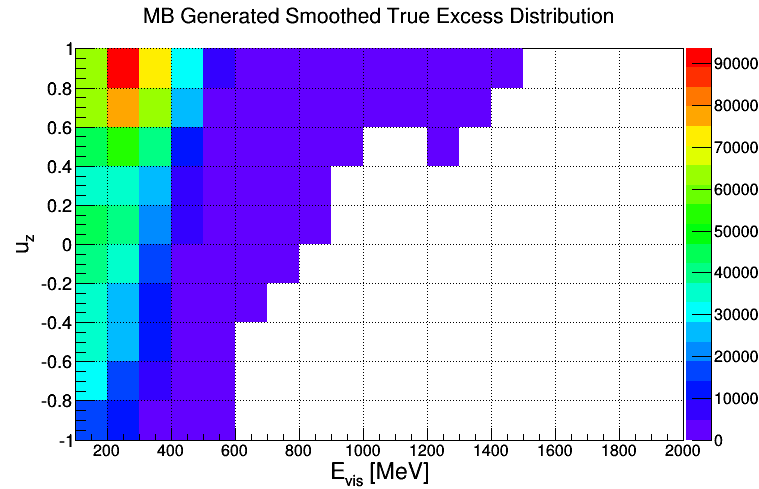
\includegraphics[width=0.9\textwidth]{Figures/miniboone_excess_th2d.png} \\
\caption{\textit{The computed distribution of $u_z$ (how foward-going the event is) vs. $E_{vis}$ for N = 1000 times the MiniBooNE low energy excess (raw) events.}}\label{MBth2dfig}
\end{figure}

While the shape of the simulated MicroBooNE signal events is determined by the above process, the absolute normalization of this sample is computed by comparing the relative size of the signal with respect to the intrinsic $\nu_e$ backgrounds as observed by MiniBooNE. This is appropriate to do only because of the assumption that the origin of the low energy excess is intrinsic BNB $\nu_e$s. From MiniBooNE data and MC, there are 187.7 excess signal events and 148.4 intrinsic $\nu_e$ events in the $E_\nu^{CCQE}$ energy range from 100 to 600 MeV (187.7/148.4=1.26). In this analysis, the number of intrinsic $\nu_e$ events in that $E_\nu^{CCQE}$ energy range in MicroBooNE is computed to be 159.8, and therefore the simulated signal sample is normalized to have 159.8*1.26=201.3 events in that $E_\nu^{CCQE}$ energy range.\\





















\subsection{Sensitivity Results}
Here I show the stacked background with the scaled signal on top, I describe how I compute a sensitivity (statistical errors only for now... I could do a back-of-the-envelope estimate of systematic errors which are dominated by flux). ``Probably do need some estimates of systematic uncertainties. Also will you say anything about an electron LEE vs a photon LEE sensitivity''.

\subsubsection{Results with Realistic Shower Reconstruction Efficiency}
Here I mention that the ``perfect reconstruction'' efficiency is 100\% but that isn't quite realistic. I'll state we assumed 80\%, and ICARUS quoted something similar. I'll describe how we emulate the non-perfect efficiency and how it isn't as simple as multiplying everything by 0.8 (for example we will get increased pi0 backgrounds when we fail to reconstruct just one of the showers).

\subsubsection{Next Steps}
Here I talk about how what's next is automated shower reconstruction being incorporated. Another important ingredient in the whole LEE analysis is constraining the nue backgrounds. The intrinsic nues which come from kaon decay can be constrained by studying numu interactions that come from kaon decay. This section will flow into the next chapter of the thesis: kaon production studies. ``Main nue background in LEE region is nue from muon decay, which is tied to the observed numu events. As you say, constaining nue from kaon decay can be constrained by the observation of the high energy numu rate, the topic of the next chapter.''



\chapter{Kaon Production Studies}
\label{sec:kaon}

This chapter of the thesis will describe a MicroBooNE analysis done with the goal of constraining the intrinsic $\nu_e$ background for the previously described low energy excess search. As shown, this is the dominant background in the search, and a significant portion of the intrinsic $\nu_e$ background comes from kaon decay in the booster neutrino beam-line. The systematic uncertainty on the flux of $\nu_e$ from kaon decay is one of the largest uncertainties reducing the low energy excess significance. This chapter will describe how measuring the highest energy $\nu_\mu$ interactions in MicroBooNE can provide information about the kaon production in the beam-line, and constrain this important systematic. Exactly how these events are reconstructed and selected will be described, data to monte carlo comparisons will be shown, and the limitations of this analysis in its current form will be discussed.

%why we want to measure it, half of nues in search come from kaon decay, how to measure it is with high energy numus
%history: previous miniboone uncertainty on this was 40% or whatever, after gary's paper it's 14%,
%we want to explore doing the same measurement with microboone
%the general idea is to select high energy numus and compare data to MC to get a "normalization determination with improved uncertainty"
\section{BNB Kaon Production Introduction and Motivation}
As described in Chapter \ref{sec:beam}, the BNB is predominantly composed of $\nu_\mu$ (92.9\%) and $\overline{\nu}_\mu$ (6.5\%) with a small contamination of $\nu_e$ and $\overline{\nu}_e$ (0.6\% combined). The BNB flux by neutrino type at the MicroBooNE detector in neutrino-mode running is shown in Figure \ref{BNB_flux_uboone_fig}.

\begin{figure}[ht!]
\centering
	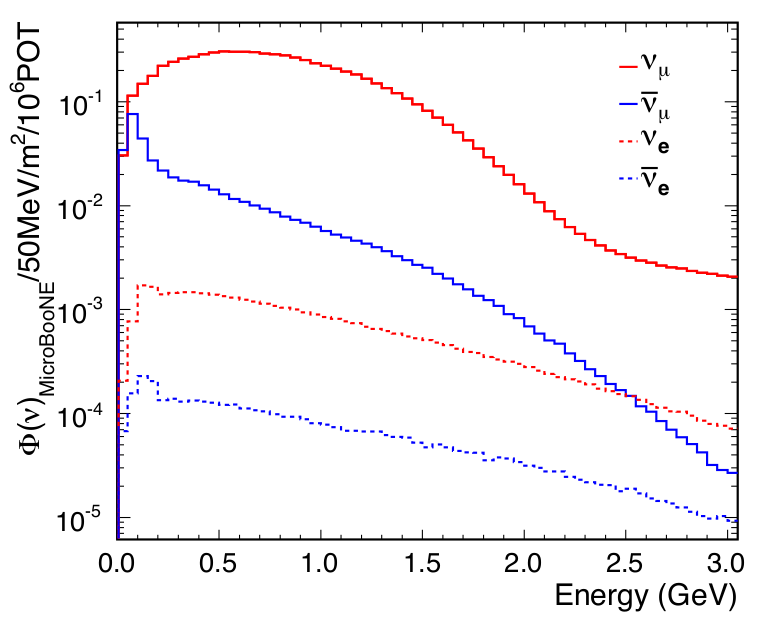
\includegraphics[width=0.9\textwidth]{Figures/BNB_flux_uboone.png} \\
\caption{\textit{The Booster Neutrino Beam (BNB) flux at MicroBooNE.}}\label{BNB_flux_uboone_fig}
\end{figure}

The decay modes producing beam $\nu_\mu$ and $\overline{\nu}_\mu$ are
\begin{itemize}
	\item $\pi^+\rightarrow\mu^++\nu_\mu$
	\item $K^+\rightarrow\mu^++\nu_\mu$
	\item $\pi^-\rightarrow\mu^-+\overline{\nu}_\mu$
\end{itemize}
and the decay modes producing beam $\nu_e$ and $\overline{\nu}_e$ are
\begin{itemize}
	\item $K^+ \rightarrow \pi^0 + e^+ + \nu_e$
	\item $\mu^+ \rightarrow e^+ + \overline{\nu}_\mu + \nu_e$
	\item $K^0_L \rightarrow \pi^- + e^+ + \nu_e$
	\item $K^0_L \rightarrow \pi^+ + e^- + \overline{\nu}_e$.
\end{itemize}

For the $\nu_\mu$ in the beam, the breakdown of $\nu_\mu$ production parentage as a function of neutrino energy is shown in Figure \ref{bnb_numu_breakdown_fig}. In the energy region $E_{\nu_\mu} < 2$ GeV, most $\nu_\mu$ come from $\pi^+$ decay, whereas at higher energies most $\nu_\mu$ come from $K^+$ decay. Therefore, the strategy to measure $K^+$ production in the beam is to select high energy $\nu_\mu$ interactions and compare simulation to data in terms of event rates in order to compute a normalization factor with an uncertainty.\\

\begin{figure}[ht!]
\centering
	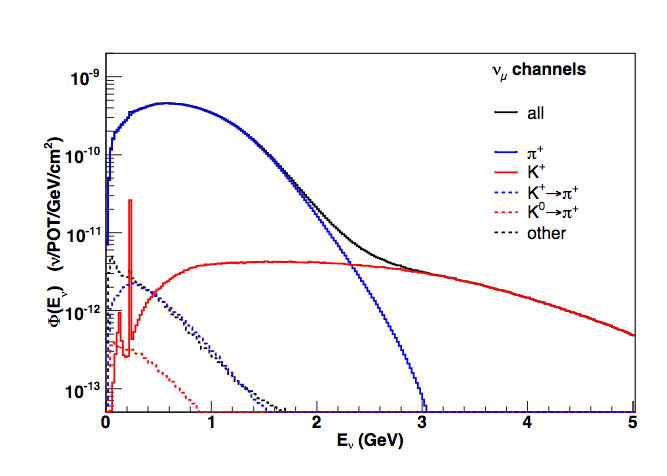
\includegraphics[width=0.9\textwidth]{Figures/bnb_numu_breakdown.png} \\
\caption{\textit{The beam $\nu_\mu$ parentage as a function of true neutrino energy.}}\label{bnb_numu_breakdown_fig}
\end{figure}

In the initial MiniBooNE publications, the systematic uncertainty on the intrinsic $\nu_e$ from $K^+$ decay in the beam was 40\%. This systematic came from several sources in the beam simulation process including proton delivery/optics, secondary particle productions, hadronic interactions in the target or horn, and horn magnetic field. The uncertainty in pion production was determined from spline fits to external HARP pion double differential cross section data using the Sanford-Wang (SW) parametrization \cite{SanfordWangGary7} \cite{HARPgary8}. There was no published external data for $K^+$ production at the BNB primary proton beam energy of 8 GeV, so the Feynman scaling hypothesis was used to extrapolate $K^+$ production measurements to this energy \cite{FEYNMANgary6}. Following a measurement by the SciBooNE collaboration \cite{gary_kaon_production_paper}, this uncertainty was reduced to 14\%. Even with this drastic reduction, $K^+$ production is still the largest source of uncertainty for BNB $\nu_e$ above neutrino energies of around 0.6 GeV, as shown in Figure \ref{UB_nue_fluxerror_fig}. The analysis described in the following sections aims to reproduce the SciBooNE measurement, but with the MicroBooNE detector. Reproducing this is important not only to further constrain this dominant systematic uncertainty for higher energy $\nu_e$ interactions, but also because MicroBooNE is has a different target material and different detector systematics. Additionally, the referenced analysis involved using the NUANCE neutrino interaction simulation library, whereas MicroBooNE uses a different package called GENIE.

\begin{figure}[ht!]
\centering
	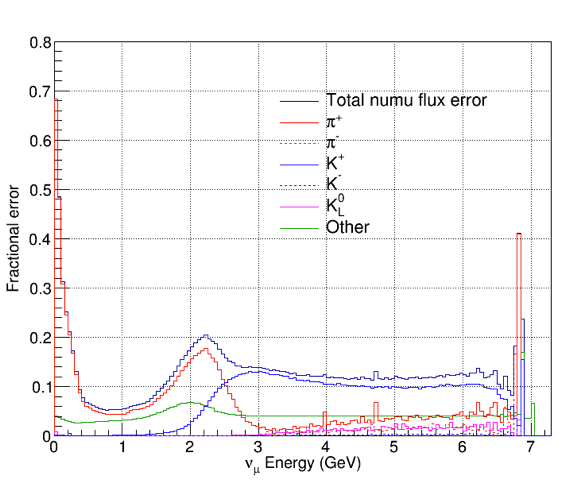
\includegraphics[width=0.9\textwidth]{Figures/UB_nue_fluxerror.png} \\
\caption{\textit{The fractional error for each neutrino species in the BNB at the MicroBooNE detector. Note the largest uncertainty at higher $\nu_\mu$ energies still comes from $K^+$ production, even including the SciBooNE measurement.}}\label{UB_nue_fluxerror_fig}
\end{figure}


\section{Event Selection}
The topologies of interest for this analysis are charge-current $\nu_\mu$ interactions in the MicroBooNE TPC. In such interactions, a $\nu_\mu$ interacts with a nucleon in an argon atom, exchanging a charged boson. Which particles exit the interaction depend on interaction channel and final state interactions, but in general these events have a muon in the final state. The relative probability of interaction type (quasi-elastic $QE$, resonant production $RES$, or deep inelastic scattering $DIS$) can be inferred from Figure \ref{bnb_xsec_breakdown_fig}. While most $\nu_\mu$ interactions in the dominant BNB energy region peaked at 0.7 GeV are quasi-elastic in nature, resonant production and deep inelastic scattering become more probable at higher neutrino energies.\\

\begin{figure}[ht!]
\centering
	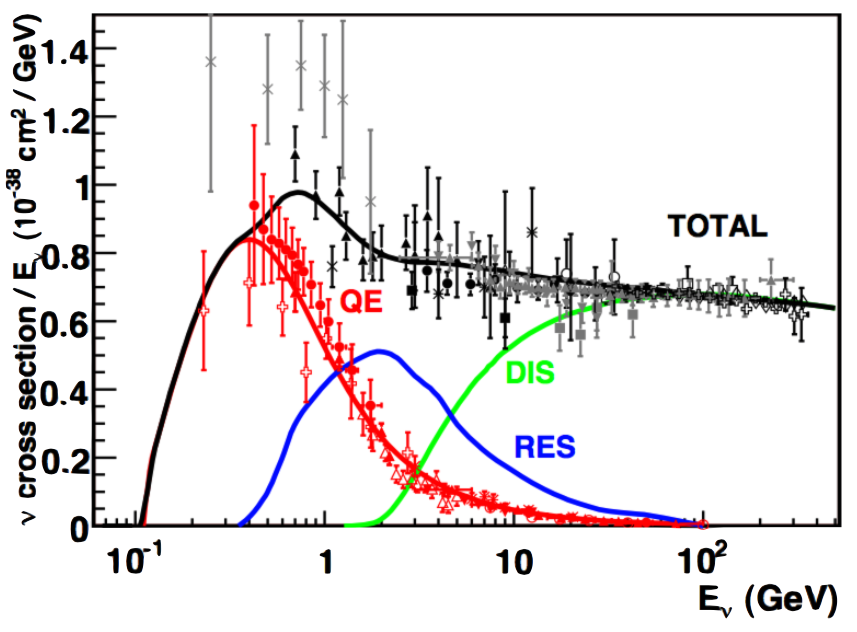
\includegraphics[width=0.9\textwidth]{Figures/numu_xsec_breakdown.png} \\
\caption{\textit{Muon neutrino charged-current cross section measurements and predictions as a function of neutrino energy.}}\label{bnb_xsec_breakdown_fig}
\end{figure}

The strategy is to select $\nu_\mu$ interaction events in MicroBooNE, reconstruct the neutrino energy, and then place a minimum energy cut to obtain a pure sample of $\nu_\mu$ events originating from kaon decay in the beam-line. The interaction reconstruction, selection criteria, and neutrino energy definition are described in the following subsections.

\subsection{Track Reconstruction}
This section provides a brief overview of how particles traversing the detector medium are physically observed and are reconstructed in software. For a thorough description of the MicroBooNE detector, see Section \ref{sec:detector}.\\

In a $\nu_\mu^{CC}$ (charge current) interaction, a muon exits the interaction vertex. This particle leaves a trail of ionization electrons that create a relatively straight-line pattern in three dimensions. This line of ionization electrons is referred to as a track. Other relevant particles traversing liquid argon that create tracks are protons and charged pions. These ionization electrons are drifted by an external electric field past three anode wire planes, situated at different angles, with 3 $mm$ spacing between each plane, and a 3 $mm$ pitch between each wire. Scintillation light from the particle is observed by photomultiplier tubes (PMTs) situated behind the anode wire planes. The signals observed on each wire plane provides a 2D image of the particle track, and combining information across multiple planes allows for complete 3D reconstruction, though there is ambiguity for the absolute location along the drift coordinate. Matching the timing of PMT signals with that of wire signals from a track clarifies this ambiguity, resulting in fully 3-dimensional reconstructed tracks.\\

The pattern recognition software used in this analysis to convert detector signals to reconstructed 3D tracks is called Pandora \cite{pandora_paper}. This package is responsible for taking reconstructed wire signals in a triggered MicroBooNE event, clustering them on each plane (with clusters representing individual particles in the event), and matching those clusters across planes to create 3D objects. In general, event reconstruction in a LArTPC is a difficult problem which the MicroBooNE collaboration has yet to fully solve. The Pandora package is a complex one which consists of a large number of nested algorithms designed to perform pattern recognition tasks, and these algorithms are not limited only to LArTPCs.\\

The output of the Pandora package that is relevant for this analysis are 3D reconstructed tracks created by Pandora's Projection Matching Algorithm (PMA), as well as 3D reconstructed interaction vertices which represent candidate neutrino interaction locations. Since $\nu_\mu^{CC}$ interactions always have a muon track exiting an interaction vertex, this is the fundamental criteria to select a sample of these events. More detailed criteria are needed to mitigate backgrounds, and the selection cuts are described in more detail in the following section.

\subsection{Selection Criteria}\label{kaon_event_selection_section}
The following selection criteria are placed on the reconstructed objects to select $\nu_\mu$ charged-current interactions in which a candidate muon track exits the interaction vertex:

\begin{enumerate}
\item The event must have at least one bright (50 photoelectron equivalent) optical flash, reconstructed from PMT timing signals, in coincidence with the expected BNB-neutrino arrival time. %1
\item The $z$ coordinate of the optical flash, as determined by the pulse height and timing of signals in the 32 PMTs, must be within 70 cm of any point on the $z$ projection of the candidate muon track. %2 
\item Two or more reconstructed tracks must originate from the same reconstructed vertex within the fiducial volume. %3
\item For events with exactly two tracks originating from the vertex, additional calorimetric criteria are applied to mitigate backgrounds from cosmic muons that arrive in time with the passage of the beam, then stop and decay to an electron that is reconstructed as a track. %4   
\item The length of the longest track associated with the interaction must be at least 15 centimeters in length.
\item For events with exactly two tracks originating from the same reconstructed vertex must not have exactly opposite directions (to within 5 degrees).
\end{enumerate}

Selection criteria (1) and (2) are necessary to mitigate backgrounds originating from cosmic rays arriving in coincidence with the expected beam-neutrino arrival time and triggering a readout. \\

Selection criteria (3) is necessary to mitigate cosmic backgrounds. Cosmics entering from outside of the TPC will often lead to reconstructed neutrino vertices very close to the TPC boundaries. The boundaries of the fiducial volume used in this analysis are set back from the six faces of the active volume by distances of between 20 and 37 cm, depending on the face. This volume was also chosen to reduce the impact of electric-field non-uniformities near the edges of the TPC \cite{SCE_publicnote}, which are relevant when reconstructing a track energy (described in the next section). The fiducial volume corresponds to a mass of 55 tons.\\

Selection criteria (3) is also necessary to address mis-identifications stemming from track reconstruction failures. There exists a sizable background in which a cosmic traverses the entire detector, but only a portion of its track gets reconstructed, mimicking the one-track topology. These one-track events are removed at the cost of $\nu_\mu^{CCQE}$ interactions in which only a muon exits the interaction vertex. Given that this analysis geared towards the highest energy $\nu_\mu$ interactions which are often in the RES or DIS channel (multi-track), this cut isn't very detrimental to the desired high neutrino energy signal.\\

Selection criteria (4) is necessary to remove the specific topology where a cosmic ray muon stops in the detector (with an increased ionization rate as it approaches its endpoint, known as a Bragg peak) and subsequently decays into an electron. This topology has two tracks exiting a ``kink'', which mimics a $\nu_\mu^{CC}$ topology. This cut leverages the presence of the Bragg peak to correctly identify the directions of the two tracks and therefore remove this event from the analysis.\\

Selection criteria (5) and (6) are additional cuts to mitigate specific track reconstruction failure modes that are present when reconstructing cosmic rays. In these failure modes, a long straight track can be broken up and reconstructed as two or more straight tracks, with a reconstructed vertex as the breaking point.\\

The above selection criteria serve only to select a sample of $\nu_\mu^{CC}$ events, which come from both pion and kaon decay. The efficiency to select events these is defined as
\begin{equation}
\epsilon_{\nu_\mu^{CC}} = \frac{\text{\# selected events}}{\text{\# true $\nu_\mu^{CC}$ events in the fiducial volume}}
\end{equation}
and the purity is defined as
\begin{equation}
\pi_{\nu_\mu^{CC}} = \frac{\text{\# true $\nu_\mu^{CC}$ correctly identified events in selected sample}}{\text{\# selected events}}.
\end{equation}
With the described selection criteria, the efficiency $\epsilon_{\nu_\mu^{CC}}$ is 27\%. This efficiency is rather low because of the requirement of two reconstructed tracks exiting the interaction combined with a low track reconstruction efficiency, especially for short tracks near the vertex. The purity is 82\%, and the primary contaminating backgrounds are those from cosmics. The backgrounds to this analysis are discussed in more detail in the following section.

\subsection{Backgrounds}
There are three main backgrounds to this $\nu_\mu^{CC}$ from $K^+$ decay search: $\nu_\mu^{CC}$ from $\pi$ decay interactions, neutral current interactions, and cosmic-induced backgrounds. The $\nu_\mu^{CC}$ from $\pi$ decay interactions are the most dominant background and will be removed with a cut on neutrino energy, which is described in the following section.\\

The neutral current backgrounds occur when a beam neutrino of any flavor interacts in such a way as to mimic a $\nu_\mu^{CC}$ interaction. For example, a neutrino can interact with a nucleus and liberate a proton and a charged pion. In this case, the charged pion may be mis-identified as a muon.\\ %Additionally, a neutrino may interact and create a neutral pion which subsequently decays into two photon showers. It is possible those showers accidentally get reconstructed as tracks, mimicking a $\nu_\mu^{CC}$ interaction.\\

The cosmic-induced backgrounds are mitigated largely by the previously described event selection cuts. Their topologies are usually caused either by track reconstruction failures, or by stopping muons which decay into electrons. In the latter example, the track direction of the muon must be incorrect, and the decay electron must be reconstructed as a separate track. Though many calorimetric and track-length based selection criteria are used to reduce this background, it still persists because the rate of stopping cosmics in triggered readouts far outweighs that of $\nu_\mu^{CC}$ interactions.\\

With the events selected, the next step is to reconstruct the neutrino energy. This is necessary because the neutrino energy is the variable through which the $\nu_\mu$ from $K^+$ decay sample of interest is isolated.

\section{Neutrino Energy Reconstruction}\label{kaon_nu_energy_section}

Event selection (Section \ref{kaon_event_selection_section}) provides a sample of candidate $\nu_\mu^{CC}$ interactions consisting of a number ($>2$) of reconstructed tracks exiting a common neutrino interaction vertex. Each track must first be associated with a particle identity (referred to as PID) in order to compute the energy of that track. Note that in $\nu_\mu^{CC}\pi^0$ interactions there will also be two showers exiting the vertex from the neutral pion decay. However, these showers (and therefore their associated energy) are ignored. The reason for this is that at the time of this analysis, the shower reconstruction performance in MicroBooNE software isn't at an adequate level to include them. Excluding them will ultimately worsen the energy reconstruction performance, but the performance is still sufficient to select a pure sample of $\nu_\mu^{CC}$ interactions from $K^+$ decay, as will be shown later.\\

The longest track in this set is assumed to be the muon, which is reasonable because on average the majority of the neutrino energy in a $\nu_\mu^{CC}$ interaction is transferred to the outgoing muon, as shown in Figure \ref{numuCC_energyfraction_tomuon_fig}. Also, muons are in general closer to minimally ionizing than to other final state particles like protons and therefore produce the longest tracks.\\

\begin{figure}[ht!]
\centering
	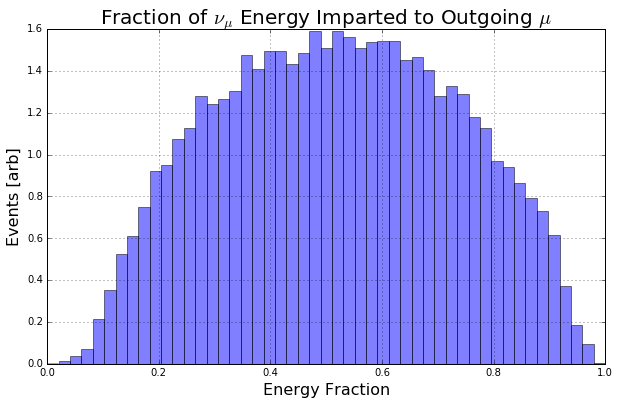
\includegraphics[width=0.9\textwidth]{Figures/numuCC_energyfraction_tomuon.png} \\
\caption{\textit{The fraction of $\nu_\mu$ energy imparted to the outgoing lepton ($\mu$) in $\nu_\mu^{CC}$ interactions.}}\label{numuCC_energyfraction_tomuon_fig}
\end{figure}

The remaining tracks exiting the interaction are classified as either charged pions, or protons. This is reasonable because only one muon can exit a $\nu_\mu^{CC}$ interaction vertex (barring negligibly rare topologies in which a charged pion is created and decays within the nucleus, resulting in two muons in the final state). Protons are much more highly ionizing than charged pions, and therefore the measured dE/dx of the tracks are used in classification; shorter, highly ionizing tracks are tagged as protons, and longer, lower ionizing tracks are tagged as charged pions.\\

The reconstructed neutrino energy is defined as the sum of the energies of all tracks exiting the interaction vertex. For muon and pion tracks, their total energies are added (including mass), while for proton tracks only the kinetic energy is added. This is because while the muons and pions are created with energy directly from the neutrino, the protons are pre-existing and are liberated from the nucleus. This simplistic energy definition neglects binding energy in the nucleus, but that effect is small.\\

The method used to reconstruct the energy of the muon track depends on whether that track is fully contained in the fiducial volume. In general, reconstructing the energies of fully contained particle tracks in a LArTPC is straightforward, either with a range-based approach, or a calorimetric approach (since calorimetric information can be gleaned from the size of sense-wire signals). In this analysis, range-based energy is used for fully contained muons. The stopping power of muons in liquid argon is well described by the continuous slowing-down approximation (CSDA) by the particle data group, and agrees with data at the sub-percent level \cite{MIPenergysource} \cite{PDG_spline_table}. By using a linear interpolation between points in the stopping power table of ref. \cite{PDG_spline_table}, the length of a track can be used to reconstruct the muon's total energy with resolution better than 4\% and negligible bias.\\

For muon tracks that exit the fiducial volume (which is ultimately the case for all selected $\nu_\mu^{CC}$ from $K^+$ decay), a different method is required to compute the track energy. This method leverages a phenomenon called multiple Coulomb scattering (MCS), and the development and characterization of this method is the subject of a pending publication by the author of this thesis in the Journal of Instrumentation. This publication comprises the following chapter of this thesis. To summarize, the MCS energy resolution for well reconstructed exiting muon tracks with at least one meter of their length contained in the fiducial volume is on the order of 15\% for muons with momenta below 2.5 GeV/c, and on the order of 30\% for muons with momenta between 2.5 and 4.0 GeV/c. A downside to the MCS method is that it requires at least a meter of track to be contained. For muons that exit with less than a meter contained, the range-based energy is necessarily used, which is often a significant underestimation of the true energy. Note that space charge effects most predominantly located near the edges of the TPC are not included in this simulation. These electric-field non-uniformities have the effect of bending a track, which will cause the MCS technique to underestimate the track's energy. To account for this difference between data and Monte-Carlo, all reconstructed tracks in this analysis are truncated to be contained within the fiducial volume, which was chosen because the effect of electric field non-uniformities are small in this region. This effectively converts the fiducial volume to an active volume, in which space charge effects are negligible.\\

Charged pion tracks are treated in much the same way as muon tracks. When they are contained, range-based energy is used, and when they exit, MCS energy is used (despite the fact that MCS energy is tuned for muons, the same method works sufficiently well for the purposes of this analysis on pions). Proton tracks are in general much shorter and therefore their probability of exiting the fiducial volume is small. For these tracks, a range-based energy is used based on the stopping power of protons in liquid argon published by the same aforementioned references.\\

Given the described event selection criteria, particle identification techniques, and track energy methods, a distribution of the reconstructed neutrino energy versus true neutrino energy for a sample of correctly identified $\nu_\mu^{CC}$ interactions in MicroBooNE simulation is shown in Figure \ref{kaon_recoenergy_2d_fig}. It can be seen that the reconstructed energy tends to be an underestimation of the true energy. This is caused by the failure to include shower-based energy from the interaction (as mentioned previously), as well as needing to use range-based energy for tracks which have less than one meter contained in the TPC. Additionally the relatively crude particle identification techniques could have an impact as well. While this reconstructed neutrino energy could certainly be improved upon, its performance is sufficient for this analysis. As you can see from the figure, placing a cut on reconstructed neutrino energy at around 2.5 GeV will provide a relatively pure sample of events in which the true neutrino energy is also above 2.5 GeV. Since this analysis is a normalization measurement (a counting experiment), the shortcomings of this neutrino energy definition are acceptable.

\begin{figure}[ht!]
\centering
	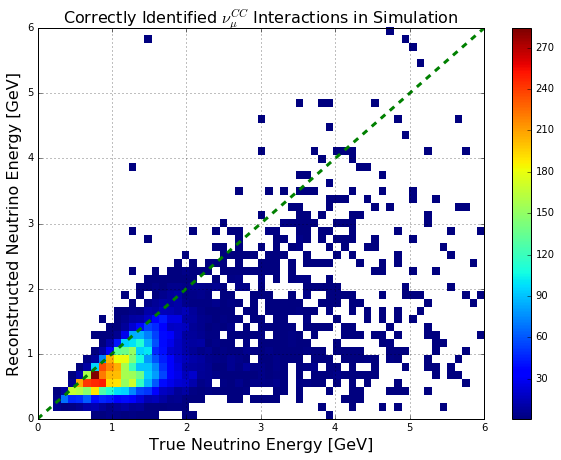
\includegraphics[width=0.9\textwidth]{Figures/kaon_recoenergy_2d.png} \\
\caption{\textit{Reconstructed neutrino energy versus true neutrino energy for a sample of correctly identified BNB $\nu_\mu^{CC}$ interactions in the MicroBooNE TPC.}}\label{kaon_recoenergy_2d_fig}
\end{figure}

\section{Results in Simulation}
The simulation used for this analysis are BNB simulated neutrino interactions within the entire MicroBooNE TPC. The BNB flux is described in Chapter \ref{sec:beam} of this thesis. The neutrino interaction event generator used is GENIE \cite{GENIEsource}. These interactions also include simulated cosmic rays by the CORSIKA package \cite{CORSIKAsource}. This ``BNB + Cosmic'' simulation provides the measurement sample as well as all relevant backgrounds. If a reconstructed neutrino vertex is within 3 cm of a true $\nu_\mu^{CC}$ interaction vertex, that event will be classified as either $\nu_\mu$ from pion decay (background) or $\nu_\mu$ from kaon decay (signal), depending on the true neutrino parent. If the reconstructed neutrino vertex is within 3 cm of a true $\nu_x^{NC}$ interaction vertex, that event is classified as a neutral current background. Lastly, if the reconstructed neutrino vertex is not near any true neutrino interaction point, the interaction is tagged as cosmic.\\

2.2 $\times 10^{20}$ protons-on-target are simulated in this analysis, and the final histograms are scaled to 0.5 $\times 10^{20}$. This scaling is done because when a comparison to data is made (in the next section), only 0.5 $\times 10^{20}$ protons-on-target worth of data are available for this analysis due to blinding schemes within the MicroBooNE collaboration. Note that the nominal amount of protons-on-target scheduled to be delivered to MicroBooNE over a three-year running period is much more than this, 6.6$\times 10^{20}$; unblinding the full data set in the future will improve the strength of this analysis' result by decreasing the statistical uncertainty. \\

The distribution of simulated signal and backgrounds as a function of reconstructed neutrino energy between 0 and 2.5 GeV (which is referred to as the sideband region for this analysis) in Figure \ref{kaon_stack_sideband_nodata}. In this stacked histogram figure, the green histogram is the signal of interest, $\nu_\mu^{CC}$ interactions from kaon decay. In this sideband region the $\nu_\mu^{CC}$ from pion decay (blue) is the dominant background, while cosmic-induced backgrounds (red) are mostly relevant at reconstructed neutrino energies below 1 GeV. Neutral current backgrounds (yellow) are sub-dominant.\\

\begin{figure}[ht!]
\centering
	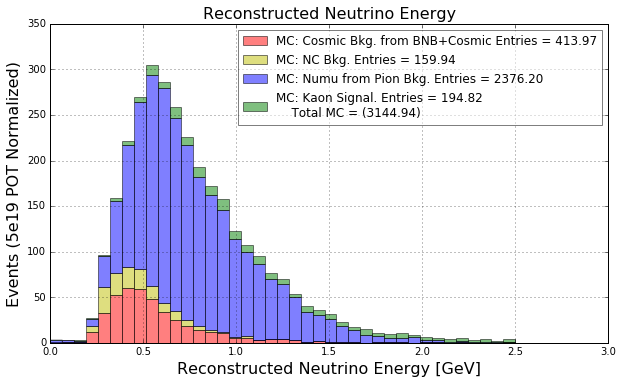
\includegraphics[width=0.9\textwidth]{Figures/kaon_simonly_sideband.png} \\
\caption{\textit{Distribution of signal (green) and backgrounds normalized for 0.5 $\times 10^{20}$ protons-on-target worth of data, for reconstructed neutrino energy below 2.5 GeV. This comprises the sideband region.}}\label{kaon_stack_sideband_nodata}
\end{figure}

In order to select a relatively pure sample of $\nu_\mu^{CC}$ from $K^+$ decay interactions, a cut on reconstructed neutrino energy is placed at 2.5 GeV. The resulting sample has a kaon signal purity of 81\%, and is shown in Figure \ref{kaon_stack_signal_nodata}. In this region, the backgrounds from neutral current interactions and from $\nu_\mu^{CC}$ from $\pi$ decay are drastically suppressed. Still remaining is a cosmic-induced background which comprises 15\% of the sample. The correlation between energy and angle of the kaons which decay to produce $\nu_\mu^{CC}$ interactions in the fiducial volume is shown in Figure \ref{all_kaon_energy_angle_2d}, and the subset of those which are reconstructed and selected in this analysis (passing the 2.5 GeV cut on neutrino energy) are shown in Figure \ref{selected_kaon_energy_angle_2d}. The projection of these distributions onto the angle axis are shown in Figure \ref{kaon_angle_selection}, and onto the energy axis in Figure \ref{kaon_energy_selection}. The mean energy and angle information for kaons which produce $\nu_\mu$ (all, and selected) and for those which produce $\nu_e$ (relevant for the electron-like low energy excess analysis) are summarized in Table \ref{kaon_energy_angle_table}. The kaons selected in the signal region tend to be skewed towards being more forward-going (smaller angle) and having higher energy, though the production phase-space is still reasonably covered by the selection (as seen by comparing Figures \ref{all_kaon_energy_angle_2d} and \ref{selected_kaon_energy_angle_2d}).
% XXX here i discuss that we use genie whereas sciboone used NUANCE which is an important difference. also mention that the simulated samples are BNB+cosmic overlayed with corsika, each event has neutrino interaction in it and associated POT. describe how in real data only like 1/6 triggers have a neutrino, and describe how we handle the relative normalization of that (beam on minus beam off).

%

\begin{figure}[ht!]
\centering
	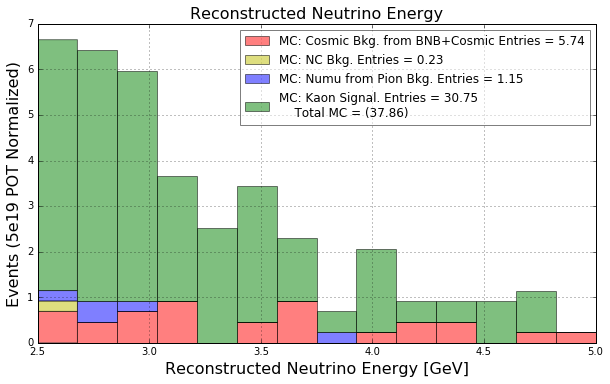
\includegraphics[width=0.9\textwidth]{Figures/kaon_simonly_signal.png} \\
\caption{\textit{Distribution of signal (green) and backgrounds normalized for 0.5 $\times 10^{20}$ protons-on-target worth of data, for reconstructed neutrino energy between 2.5 GeV and 5 GeV. This comprises the signal region, which has an 81\% purity of $\nu_\mu^{CC}$ interactions from $K^+$ decay in the beam.}}\label{kaon_stack_signal_nodata}
\end{figure}


\begin{figure}[ht!]
\centering
	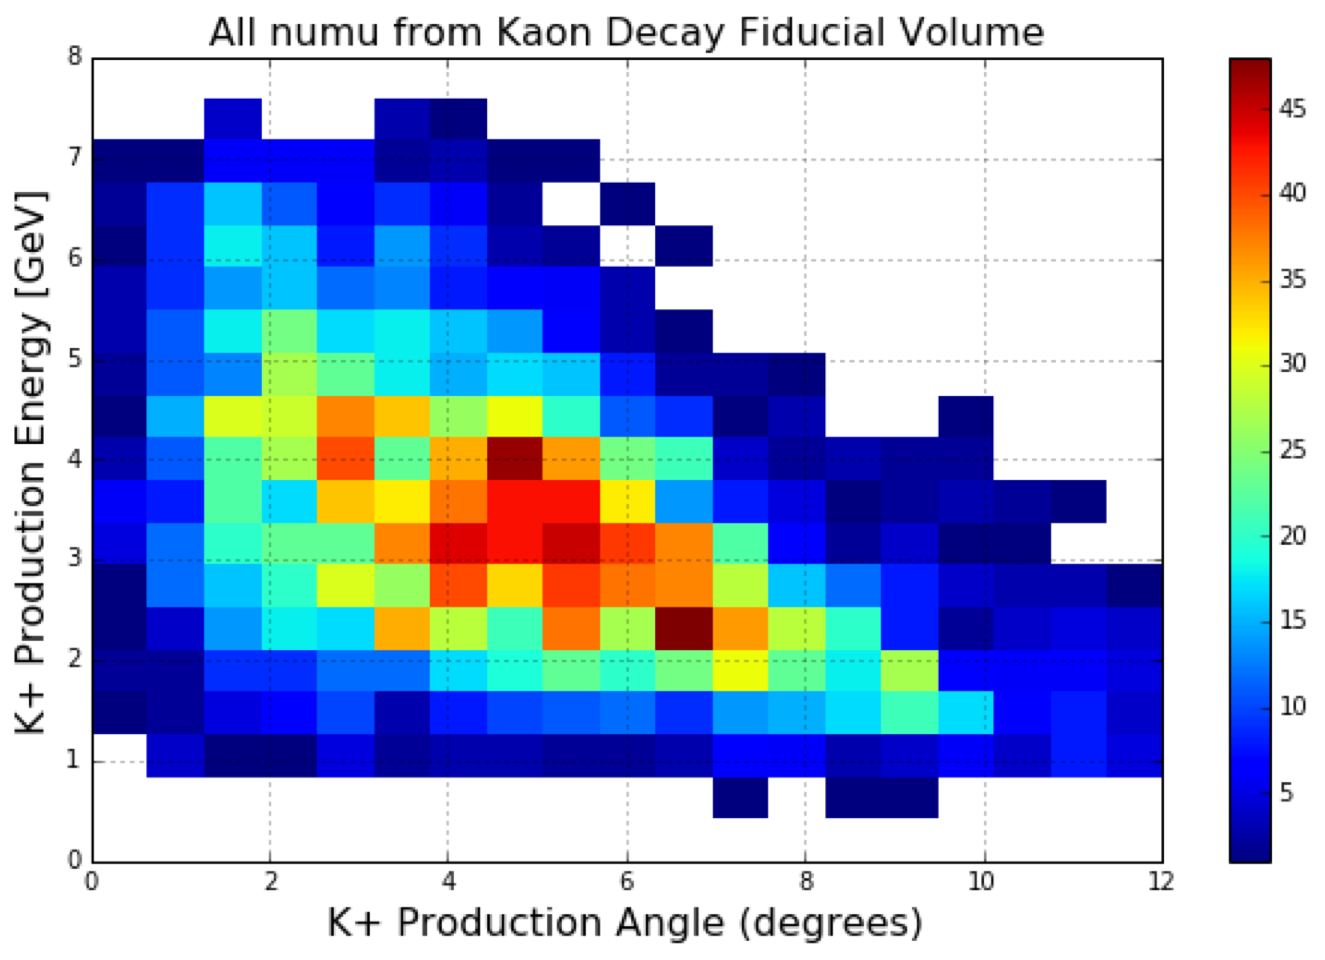
\includegraphics[width=0.9\textwidth]{Figures/all_kaon_energy_angle_2d.png} \\
\caption{\textit{A two-dimensional plot of energy versus angle for all kaons in the beam producing $\nu_\mu^{CC}$ interactions in the detector.}}\label{all_kaon_energy_angle_2d}
\end{figure}


\begin{figure}[ht!]
\centering
	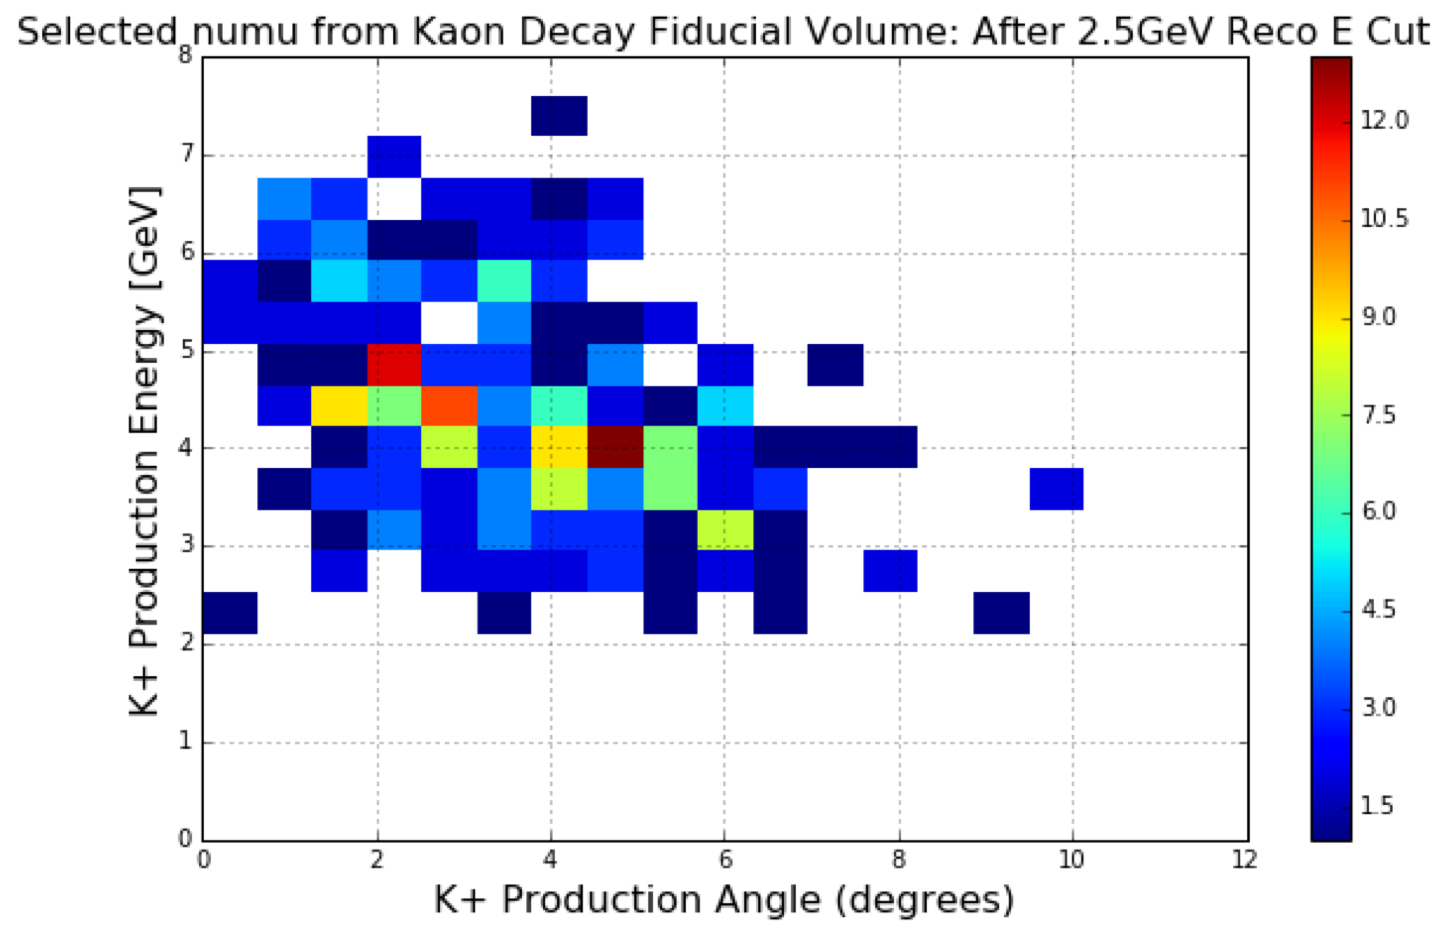
\includegraphics[width=0.9\textwidth]{Figures/selected_kaon_energy_angle_2d.png} \\
\caption{\textit{A two-dimensional plot of energy versus angle for the subset of kaons in Figure \ref{all_kaon_energy_angle_2d} which are reconstructed and selected for this analysis (having reconstructed neutrino energy above 2.5 GeV).}}\label{selected_kaon_energy_angle_2d}
\end{figure}


\begin{figure}[ht!]
\centering
	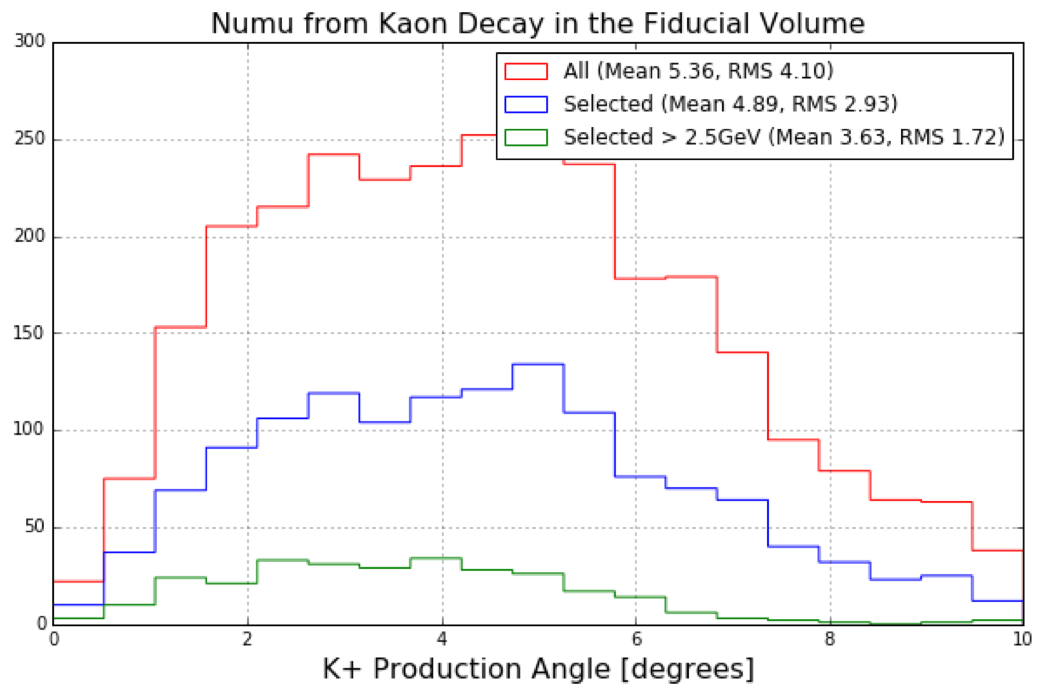
\includegraphics[width=0.9\textwidth]{Figures/kaon_angle_selection.png} \\
\caption{\textit{The kaon production angle distribution for all kaons in the beam producing $\nu_\mu^{CC}$ interactions in the detector (red), the subset of those which are reconstructed and selected in both the sideband and signal region (blue) and the subset of those in the Kaon enriched signal sample, with reconstructed neutrino energy above 2.5 GeV (green).}}\label{kaon_angle_selection}
\end{figure}


\begin{figure}[ht!]
\centering
	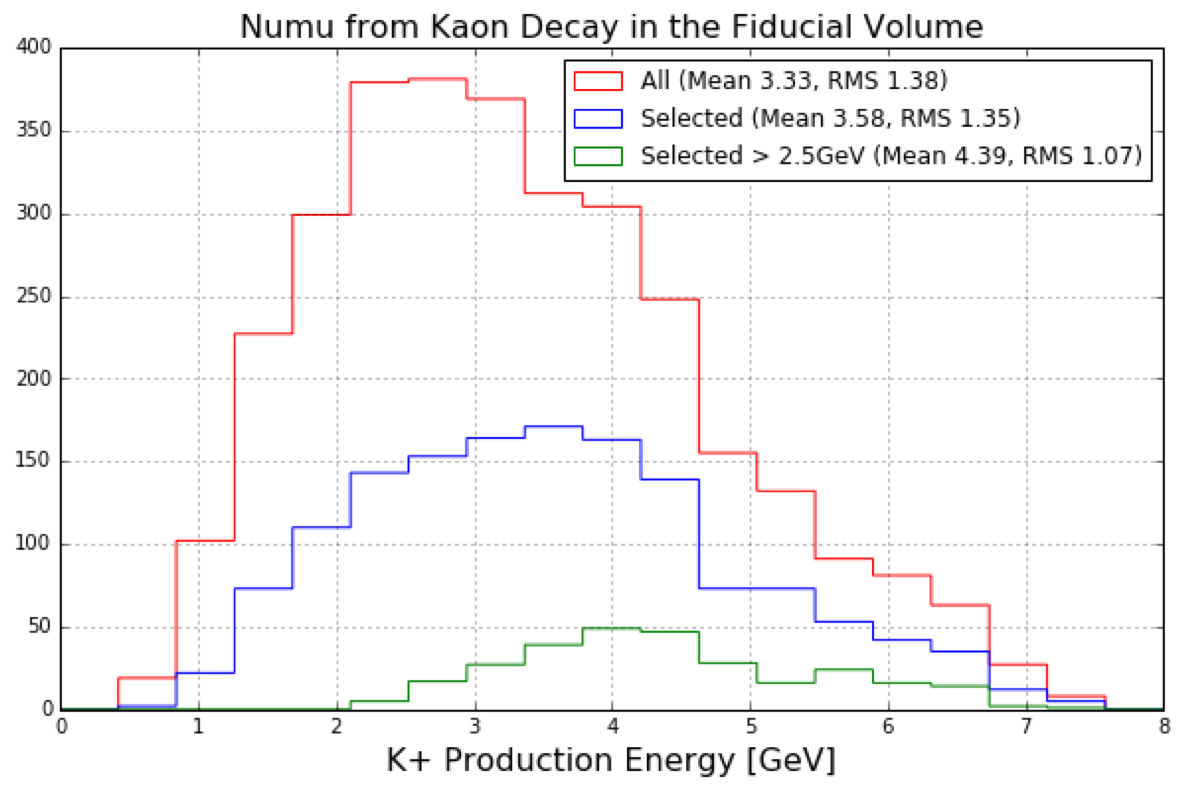
\includegraphics[width=0.9\textwidth]{Figures/kaon_energy_selection.png} \\
\caption{\textit{The kaon production energy distribution for all kaons in the beam producing $\nu_\mu^{CC}$ interactions in the detector (red), the subset of those which are reconstructed and selected in both the sideband and signal region (blue) and the subset of those in the Kaon enriched signal sample, with reconstructed neutrino energy above 2.5 GeV (green).}}\label{kaon_energy_selection}
\end{figure}


\begin{table}
\begin{tabular}{ |p{0.5cm}|p{2.5cm}|p{4cm}|p{3cm}|p{3.5cm}|  }
 \hline
 \multicolumn{5}{|c|}{Kaon Production Summary} \\
 \hline
   & All $\overline{K_\theta}$ [deg] & Selected $\overline{K_\theta}$ [deg] & All $\overline{K_E}$ [GeV] & Selected $\overline{K_E}$ [GeV]\\
 \hline \hline
 $\nu_\mu$ & 5.36 [4.10] & 3.63 [1.72] & 3.33 [1.38] & 4.39 [1.07] \\\hline
 $\nu_e$ & 5.10 [3.68] & N/A & 3.32 [1.28] & N/A \\\hline
 \hline
\end{tabular}
\caption{\textit{A summary of the mean kaon production angle ($\overline{K_\theta}$) and energy ($\overline{K_E}$) in the BNB for $\nu_\mu$ interactions (all interactions interacting within the TPC, and the subset of those which are selected in the analysis), and for $\nu_e$ interactions (providing backgrounds to the electron-like low energy excess search). Reported in brackets is the RMS of each distribution.}}\label{kaon_energy_angle_table}
\end{table}


















\section{Sideband Data and Simulation Comparisons}
As shown in the previous section, the event reconstruction and selection is able to provide a relatively pure signal sample of $\nu_\mu^{CC}$ from kaon decay interactions in the detector by choosing those with reconstructed neutrino energy above 2.5 GeV. While the sideband region (with reconstructed neutrino energy below 2.5 GeV) is composed primarily of backgrounds from $\nu_\mu^{CC}$ from $\pi$ decay interactions, it is used for lower-level comparisons between data and simulation to increase confidence in results from the signal region. This section will show several such comparison plots.\\

In order to compare data to simulation, there is a subtlety involving the cosmic background which needs to be accounted for. In the simulation, each triggered readout event has a neutrino interacting somewhere within the TPC, along with several simulated cosmic rays. However, in real data, the majority of triggers are induced by cosmic interactions arriving during the expected neutrino arrival timing window ($1.6\mu s$), and do not contain a neutrino interaction at all. To account for this, a sample of data is taken when the neutrino beam is turned off, in order to get an estimate of the cosmic background. This ``off-beam'' data is then subtracted from the ``on-beam'' data in the analysis, and the difference is what is directly comparable to simulation. The normalization factor between ``off-beam'' and ``on-beam'' data is computed based on the number of measured bright reconstructed optical flashes within the expected neutrino arrival window both during ``off-beam'' (cosmic-only) runs and ``on-beam'' runs. This factor is computed to be 0.844, which means that 84\% of triggered BNB readouts relevant to this analysis in MicroBooNE data are cosmic-induced. Note that while subtracting ``off-beam'' data from ``on-beam'' data accounts for the cosmic backgrounds not taken included in simulation, there still exists a cosmic background originating from readouts which are truly triggered by a neutrino interaction, but a cosmic arriving during the milliseconds-long readout window is mistakenly identified as the neutrino interaction. This is the background shown in red in the previously shown stacked histograms. In the forthcoming data-MC comparison plots, the ``off-beam'' data points are shown in cyan for reference only; they are already subtracted from the ``on-beam'' data when they are drawn in purple.\\

The first low level data to simulation comparison done in the sideband region is shown in Figure \ref{kaon_sideband_comp_tracklength}. This plot shows the simulated background and signals as a stacked histogram with the same color-coding as shown previously (Figure \ref{kaon_stack_sideband_nodata}). Shown in cyan is this distribution for events selected from ``off-beam'' data, which are purely cosmic mis-identifications. These points are shown only for reference. The purple data points represent ``on-beam'' minus ``off-beam'' distributions and therefore already have the cyan points subtracted out. Statistical error bars are drawn on the purple data points, taking into account statistics from both the ``on-beam'' and ``off-beam'' samples. We see a normalization difference between data and simulation of about 8\%, with data having fewer events than expected in simulation. This normalization difference in the sideband serves as a calibration factor to be applied to the signal region. Below the main figure is a bin-by-bin ratio plot of data divided by simulation. The agreement is reasonable for this variable, with the ratio generally agreeing with unity to within (statistical) uncertainty.\\


\begin{figure}[ht!]
\centering
	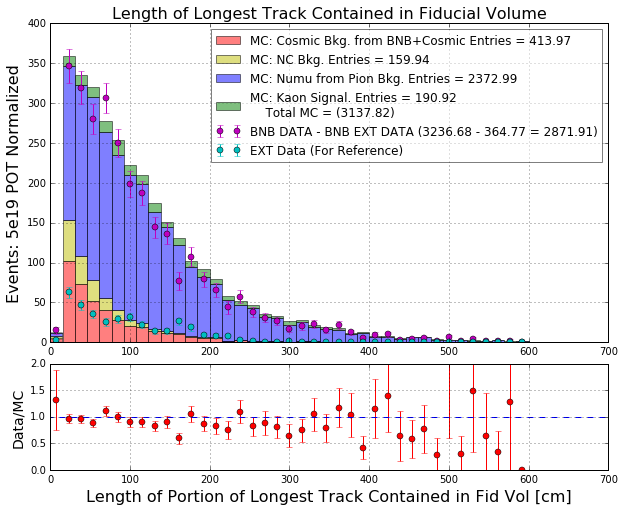
\includegraphics[width=0.9\textwidth]{Figures/kaon_sideband_comp_tracklength.png} \\
\caption{\textit{The distribution of length of the longest track associated with the interaction contained within the fiducial volume for simulated backgrounds and signal (solid histograms) overlaid with data measurements (``on-beam'' minus ``off-beam'' drawn in purple) for the sideband region in which reconstructed neutrino energy is less than 2.5 GeV. Statistical error bars are drawn on the data points, taking into account statistics from both the ``on-beam'' and ``off-beam'' samples.}}\label{kaon_sideband_comp_tracklength}
\end{figure}

The next low-level data to simulation comparison in the sideband region is shown in Figure \ref{kaon_sideband_comp_multiplicity}. This is the track multiplicity (the number of reconstructed tracks associated with the interaction). The same normalization offset of 8\% persists (since these are the same events as in Figure \ref{kaon_sideband_comp_tracklength}). While data and simulation agree for three-track events, they begin to disagree for other multiplicities. The reason for this could be imperfect modeling of nuclear interactions (including final-state intra-nuclear interactions) within the neutrino interaction simulation package.\\

\begin{figure}[ht!]
\centering
	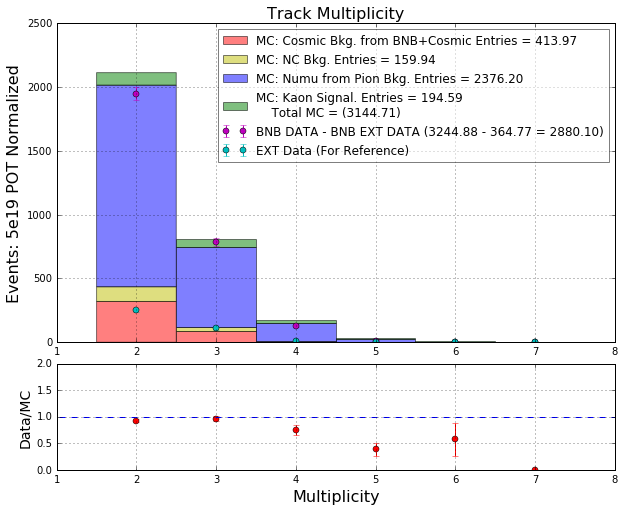
\includegraphics[width=0.9\textwidth]{Figures/kaon_sideband_comp_multiplicity.png} \\
\caption{\textit{The distribution of track multiplicity (number of tracks associated with the interaction) for simulated backgrounds and signal (solid histograms) overlaid with data measurements (``on-beam'' minus ``off-beam'' drawn in purple) for the sideband region in which reconstructed neutrino energy is less than 2.5 GeV. Statistical error bars are drawn on the data points, taking into account statistics from both the ``on-beam'' and ``off-beam'' samples.}}\label{kaon_sideband_comp_multiplicity}
\end{figure}

The next two data to simulation comparisons in the sideband region are shown in Figures \ref{kaon_sideband_comp_phi} and \ref{kaon_sideband_comp_theta}. In these plots, the difference between data and simulation becomes sizable. The first plot is the $\phi$ angle of the muon track associated with the interaction, where $\phi$ is measured in radians with respect to the vertical, around the beam direction. Naively the shape of this distribution should be flat, but the dips at $\pm\frac{\pi}{2}$ correspond to tracks oriented along the drift direction, which are difficult to reconstruct because of the geometry of the sense wires. The second plot is the $\theta$ angle of the muon track, measured with respect to the beam direction. A clear deficit of forward-going tracks (with small $\theta$) can be seen in data, with an excess of vertically-oriented tracks (with $\theta\approx\frac{\pi}{2}$). This difference between data and simulation is particularly important because the high energy $\nu_\mu^{CC}$ interactions which comprise the kaon-enriched signal region have generally very forward-going muons.\\

\begin{figure}[ht!]
\centering
	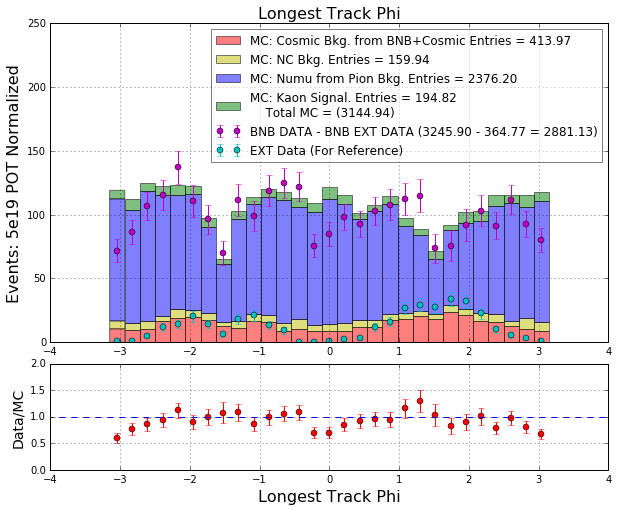
\includegraphics[width=0.9\textwidth]{Figures/kaon_sideband_comp_phi.png} \\
\caption{\textit{The distribution of $\phi$ angle (measured with respect to the vertical) of the longest track associated with the interaction for simulated backgrounds and signal (solid histograms) overlaid with data measurements (``on-beam'' minus ``off-beam'' drawn in purple) for the sideband region in which reconstructed neutrino energy is less than 2.5 GeV. Statistical error bars are drawn on the data points, taking into account statistics from both the ``on-beam'' and ``off-beam'' samples.}}\label{kaon_sideband_comp_phi}
\end{figure}


\begin{figure}[ht!]
\centering
	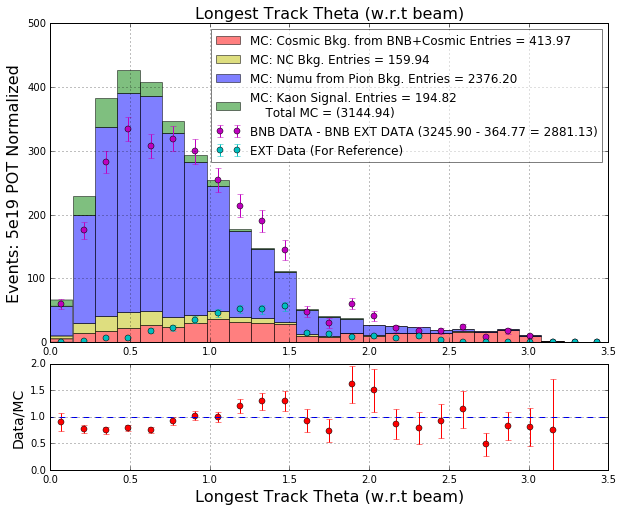
\includegraphics[width=0.9\textwidth]{Figures/kaon_sideband_comp_theta.png} \\
\caption{\textit{The distribution of $\theta$ angle (measured with respect to the beam direction) of the longest track associated with the interaction for simulated backgrounds and signal (solid histograms) overlaid with data measurements (``on-beam'' minus ``off-beam'' drawn in purple) for the sideband region in which reconstructed neutrino energy is less than 2.5 GeV. Statistical error bars are drawn on the data points, taking into account statistics from both the ``on-beam'' and ``off-beam'' samples.}}\label{kaon_sideband_comp_theta}
\end{figure}

The last low level data to simulation comparison is the computed multiple Coulomb scattering (MCS) momentum of the muon track. This distribution includes only tracks with at least one meter contained in the fiducial volume, as having this much track visible is necessary for the MCS technique to work. In this distribution there is a systematic offset in the reconstructed momentum, with that in data being shifted lower than that in simulation. Since MCS momentum is a key ingredient in computing the neutrino energy (Section \ref{kaon_nu_energy_section}), this data to simulation disagreement is particularly important. For this reason, an extensive analysis of the MCS algorithm including data to simulation comparisons was conducted by the author of this thesis. This analysis improved the performance of the algorithm, including an important change to the underlying phenomenological formula not yet discovered by other LArTPC experiments using the MCS technique. This analysis is expected to be published in the Journal of Instrumentation, and the article is included in Chapter \ref{sec:MCS} of this thesis.\\

\begin{figure}[ht!]
\centering
	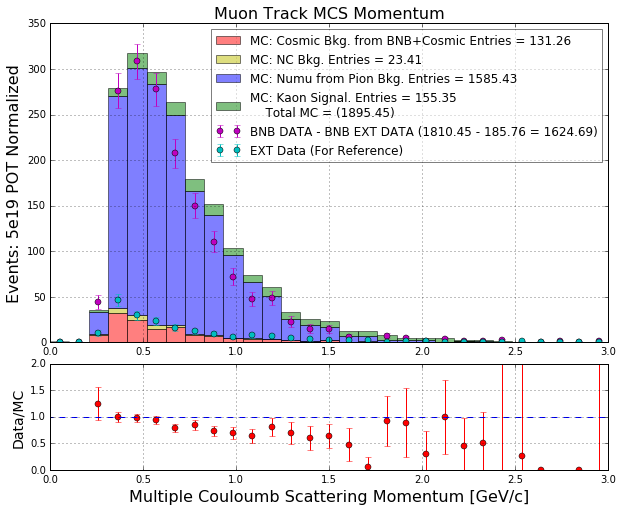
\includegraphics[width=0.9\textwidth]{Figures/kaon_sideband_comp_MCS.png} \\
\caption{\textit{The distribution of multiple Coulomb scattering computed energy for the longest track associated with the interaction for simulated backgrounds and signal (solid histograms) overlaid with data measurements (``on-beam'' minus ``off-beam'' drawn in purple) for the sideband region in which reconstructed neutrino energy is less than 2.5 GeV. Statistical error bars are drawn on the data points, taking into account statistics from both the ``on-beam'' and ``off-beam'' samples.}}\label{kaon_sideband_comp_MCS}
\end{figure}


Despite extensive studies to uncover the underlying causes of the data to simulation disparities and to fix them and/or calibrate them out, the differences remain. Since MicroBooNE is in part an R\&D experiment paving the way for future LArTPC experiments, understanding these differences are a problem that the MicroBooNE collaboration is still working to solve.\\

The comparison of data to simulation in terms of reconstructed neutrino energy for the sideband region is shown in Figure \ref{kaon_stack_sideband_both}. Given the clear systematic shift in energy to lower values in data, any measurement coming from the signal region (which is a small tail at high energies) will have an extremely large systematic uncertainty associated with it. For completeness, the reconstructed energy in the signal region is shown in Figure \ref{kaon_stack_signal_both}. While the referenced SciBooNE result predicts the $K^+$ production rate in simulation is underestimated by a factor of $0.85\pm0.11$ \cite{gary_kaon_production_paper}, the underestimation of data with respect to simulation seen in this analysis is likely not indicative of incorrectly simulated kaon production in the beam-line, but instead due to systematic detector and reconstruction effects that have not yet been solved. %Including an 8\% normalization correction derived from integrating the sideband simulation with respect to data, with 10.8 measured data events in this region, 7.12 expected backgrounds, and 30.75 expected signal events, the kaon production in simulation appears to be underestimated by a factor of
% \begin{equation}
% K^+\text{ rate} = \frac{(10.8 \times 1.08) - 7.12}{30.75} = 0.148
% \end{equation}


\begin{figure}[ht!]
\centering
	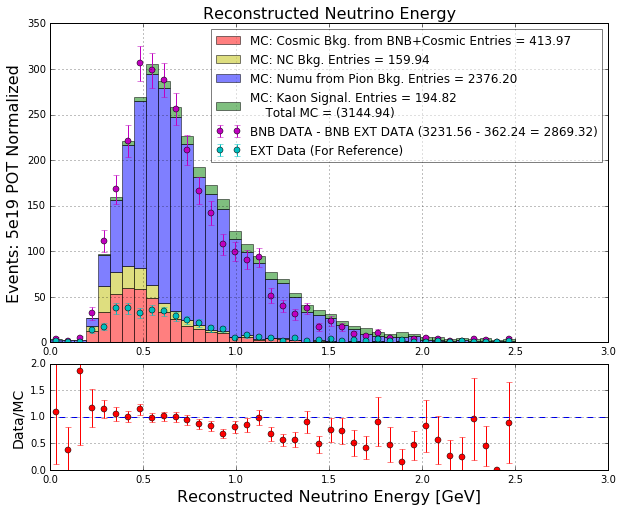
\includegraphics[width=0.9\textwidth]{Figures/kaon_both_sideband.png} \\
\caption{\textit{The distribution of reconstructed neutrino energy for simulated backgrounds and signal (solid histograms) overlaid with data measurements (``on-beam'' minus ``off-beam'' drawn in purple) for the sideband region in which reconstructed neutrino energy is less than 2.5 GeV. Statistical error bars are drawn on the data points, taking into account statistics from both the ``on-beam'' and ``off-beam'' samples.}}\label{kaon_stack_sideband_both}
\end{figure}


\begin{figure}[ht!]
\centering
	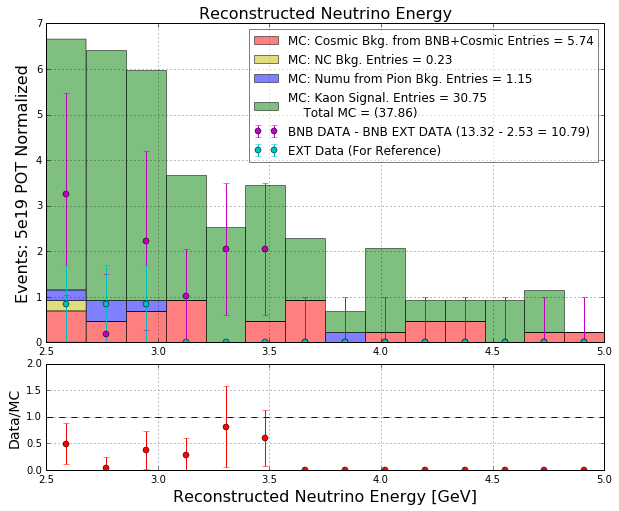
\includegraphics[width=0.9\textwidth]{Figures/kaon_both_signal.png} \\
\caption{\textit{The distribution of reconstructed neutrino energy for simulated backgrounds and signal (solid histograms) overlaid with data measurements (``on-beam'' minus ``off-beam'' drawn in purple) for the signal region in which reconstructed neutrino energy is greater than 2.5 GeV. Statistical error bars are drawn on the data points, taking into account statistics from both the ``on-beam'' and ``off-beam'' samples.}}\label{kaon_stack_signal_both}
\end{figure}

\section{Conclusions}
This thesis chapter has outlined an analysis geared towards measuring the kaon production in the beam-line by MicroBooNE, an important measurement used to constrain a main intrinsic $\nu_e$ background in the electron-like low energy excess search described in Chapter \ref{sec:LEEsensitivity}. Though a similar measurement was previously done by the SciBooNE collaboration, this measurement is important because it is done \textit{in situ} with the same detector that will search for the excess. The method used in this analysis is to select the highest energy $\nu_\mu^{CC}$ interactions within the detector in order to obtain a pure sample of $\nu_\mu$ from $K^+$ decay. The method was demonstrated to be viable in order to make a measurement with comparable significance as that of SciBooNE, though ultimately discrepancies between data and simulation in the analysis were large enough to make an absolute measurement impossible at this time. These differences are still being investigated by the MicroBooNE collaboration, and once they are understood this important analysis can proceed. One of the most important discrepancies lies within the calculation of muon momentum via multiple Coulomb scattering (MCS), since this momentum determination method is the only technique by which the momentum of a muon that exits the TPC can be calculated, and the muons from the high neutrino energy interactions in the kaon enriched signal sample all exit the TPC. A detailed study of the MCS algorithm was conducted by the author of this thesis and has been submitted for publication to the Journal of Instrumentation (JINST). This publication is presented as the following chapter of this thesis.



\chapter{Multiple Coulomb Scattering}
\label{sec:MCS}
This chapter consists of a copy of an analysis recently submitted for publication by the MicroBooNE collaboration primarily authored by the thesis author which discusses in detail the algorithm used to compute the momentum of tracks in a LArTPC by means of multiple Coulomb scattering. This is a crucial part of the previously described kaon production measurement, which in turn is a crucial part of constraining the sizable intrinsic $\nu_e$ from kaon decay background in the electron-like low energy excess search. The title of the publication is ``Determination of muon momentum in the MicroBooNE LArTPC using an improved model of multiple Coulomb scattering''.


\section{Introduction and motivation}\label{sec:intro}

In this paper we summarize the theory of multiple Coulomb scattering (MCS) and describe how the underlying Highland formula is retuned based on Monte Carlo simulation for use in liquid-argon time-projection chambers (LArTPCs). We present a maximum likelihood based algorithm that is used to determine the momentum of particles in a LArTPC. The only way to determine the momentum of a particle that exits the active volume of a LArTPC is through MCS measurements. We demonstrate that this technique works well for a sample of fully contained muons from Booster Neutrino Beam (BNB) $\nu_\mu$ charged-current (CC) interactions, and determine the resolutions and biases of the measurement. In addition we demonstrate the performance of the method on simulated exiting tracks.\\

MicroBooNE (Micro Booster Neutrino Experiment) is an experiment that uses a large LArTPC to investigate the excess of low energy events observed by the MiniBooNE experiment \cite{Aguilar-Arevalo:2013pmq} and to study neutrino-argon cross-sections. MicroBooNE is the first detector of the Short-Baseline Neutrino (SBN) \cite{SBNwhitepaper} physics program at the Fermi National Accelerator Laboratory (Fermilab), to be joined by two other LArTPCs: the Short Baseline Near Detector (SBND) and the Imaging Cosmic And Rare Underground Signal (ICARUS) detector \cite{ICARUS_maincitation}. MicroBooNE also performs important research and development in terms of detector technology and event reconstruction techniques for future LArTPC experiments including DUNE (Deep Underground Neutrino Experiment) \cite{DUNE_citation}.\\



The MicroBooNE detector \cite{ub_detectorpaper} consists of a rectangular time-projection chamber (TPC) with dimensions 2.6 m $\times$ 2.3 m $\times$ 10.4 m (width $\times$ height $\times$ length) located 470 m downstream from the Booster Neutrino Beam (BNB) target \cite{BNB_citation}. LArTPCs allow for precise three-dimensional reconstruction of particle interactions. For later reference, the $z$ axis of the detector is horizontal, along the direction of the BNB, while the $x$ direction of the TPC corresponds to the drift coordinate and the $y$ direction is the vertical direction. The mass of active liquid argon contained within the MicroBooNE TPC volume is 89 tons, out of a total mass of 170 tons.\\

A set of 32 photomultiplier tubes (PMTs) and three planes of wires with 3 mm spacing at angles of 0, and $\pm$ 60 degrees with respect to the vertical are located in the TPC for event reconstruction as shown in figure \ref{detector_fig}. The cathode plane operating voltage is -70 kV. A neutrino in the beam interacts with an argon nucleus and the charged outgoing particles traverse the medium, lose energy and leave an ionization trail. The resulting ionization electrons drift in a 273 $\text{V/cm}$ electric field to the wire planes constituting the anode. The passage of these electrons through the first two wire planes induces a signal in the wires, and their collection on the third plane also generates a signal. These signals are used to create three distinct two-dimensional views (in terms of wire and time) of the event. Combining these wire signals allow for full three-dimensional reconstruction of the event, with PMT signals providing information about the absolute drift ($x$) coordinate. The boundaries of the fiducial volume used in this analysis are set back from the six faces of the active volume by distances of between 20 and 37 cm, depending on the face, to reduce the impact of electric-field non-uniformities near the edges of the TPC. This volume corresponds to a mass of 55 tons.\\

\begin{figure}[ht!]
\centering
	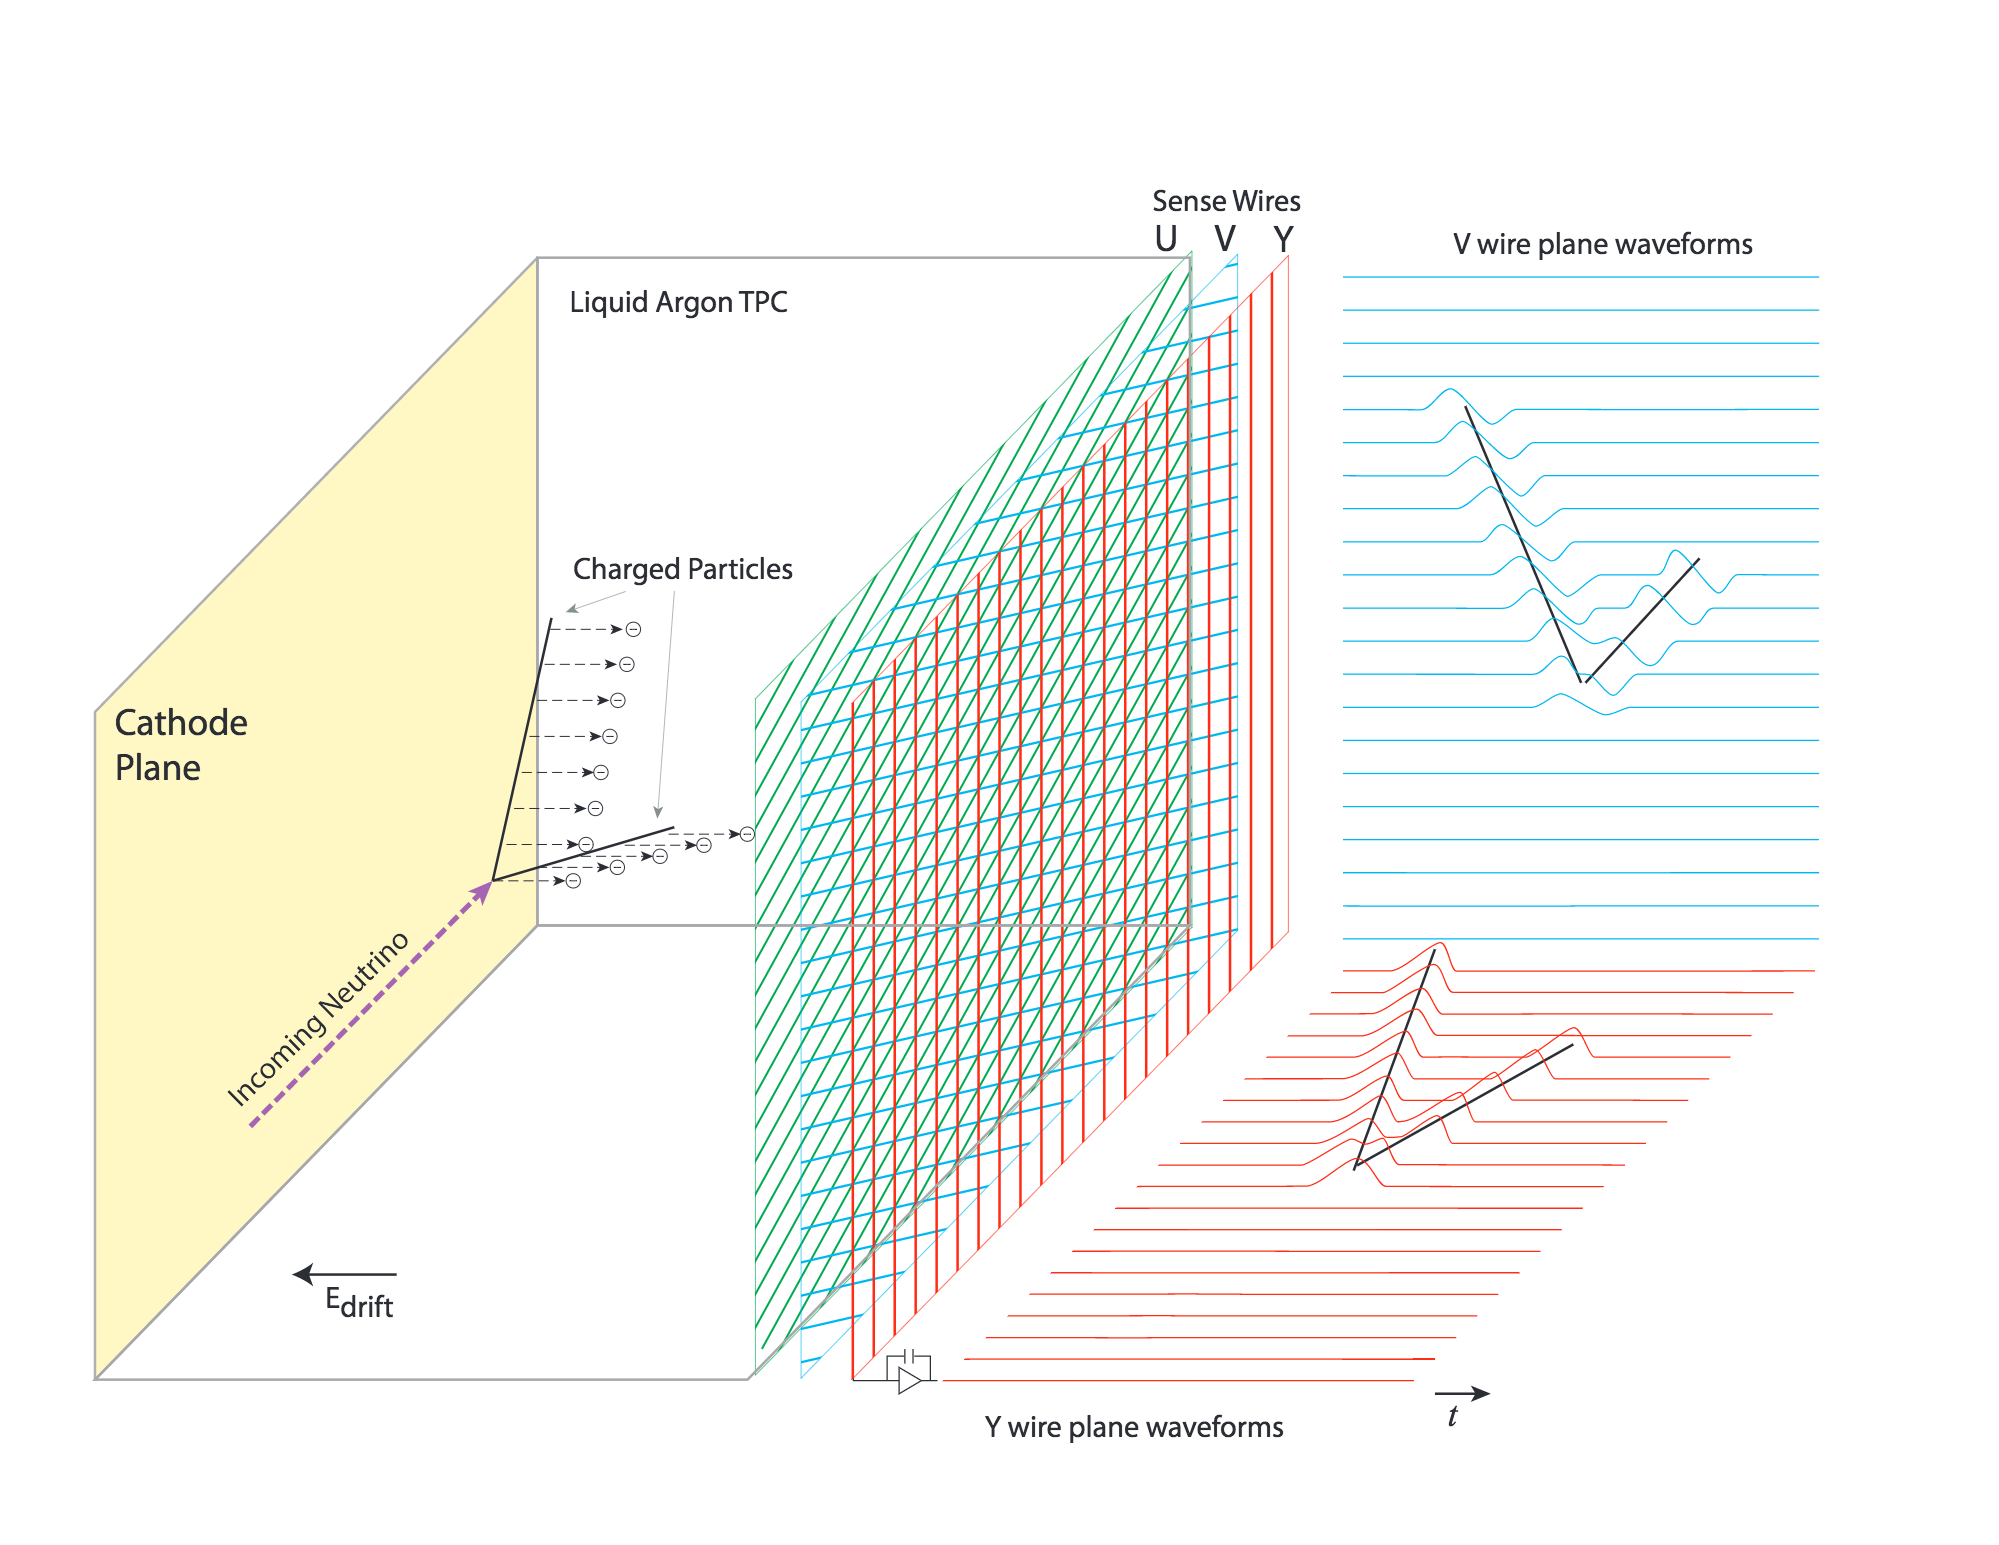
\includegraphics[width=0.9\textwidth]{Figures/MCS_PAPER_Figures/static_figs/detector2.png} \\
\caption{A diagram of the time projection chamber of the MicroBooNE detector. PMTs (not shown) are located behind the wire planes.}\label{detector_fig}
\end{figure}

The Booster Neutrino Beam (BNB) is composed predominantly of muon neutrinos ($\nu_\mu$) with a peak neutrino energy of about 0.7 GeV. Some of these neutrinos undergo charge-current ($\nu_\mu$CC) interactions in the TPC and produce muons and other particles. For muon tracks that are completely contained in the TPC, we calculate the momentum with a measurement of the length of the particle's track, or with calorimetric measurements which come from wire signal size measurements. Around half of the muons from BNB $\nu_\mu$CC interactions in MicroBooNE are not fully contained in the TPC, and therefore using a length-based or calorimetry-based method to determine the momenta for these uncontained tracks is not a possibility; the only way to determine their momenta is through MCS. \\

\section{Multiple Coulomb scattering}

Multiple Coulomb scattering occurs when a charged particle traverses medium and undergoes electromagnetic scattering off atomic nuclei. This scattering perturbs the original trajectory of the particle within the material (figure \ref{mcs_nocap_fig}). For a given initial momentum $p$, the angular deflection scatters of a particle in either the $x'$ direction or $y'$ direction (as indicated in the aforementioned figure) form a Gaussian distribution centered at zero with an RMS width, $\sigma_o^{\text{HL}}$, given by the Highland formula \cite{highland}\cite{highland-lynch-dahl} 

\begin{equation}\label{highland_eqtn}
	\sigma_o^{\text{HL}}=\frac{S_2}{p\beta c}z\sqrt{\frac{\ell}{X_0}}\left[1+\epsilon\times\ln\left(\frac{\ell}{X_0}\right)\right],
\end{equation}

\noindent where $\beta$ is the ratio of the particle's velocity to the speed of light (assuming the particle is a muon), $\ell$ is the distance traveled inside the material, $z$ is the magnitude of the charge of the particle (unity, for the case of muons), and $X_0$ is the radiation length of the target material (taken to be a constant $14$~cm in liquid argon). $S_2$ and $\epsilon$ are parameters determined to be 13.6 MeV and 0.0038, respectively. In this study, a modified version of the Highland formula is used that includes a detector-inherent angular resolution term, $\sigma_o^{\text{res}}$
\begin{equation}\label{modified_highland_eqtn}
\sigma_{o} = \sqrt{ (\sigma_o^{\text{HL}})^2 + (\sigma_o^{\text{res}})^2}.
\end{equation}
For this analysis, the $\sigma_o^{\text{res}}$ term is given a fixed value of 3 mrad which has been determined to be an acceptable value based on MicroBooNE simulation studies of muons at higher momenta. At 4.5 GeV/c muon momentum and $l\approx X_0$, equation \ref{highland_eqtn} predicts an RMS angular scatter of 3 mrad, comparable to the detector resolution. The fully contained muons addressed in this analysis have momenta below $1.5$~$\text{GeV/c}$, making the impact of this detector resolution minimal for that sample.\\

With the Highland formula, the momentum of a track-like particle can be determined using only the 3D reconstructed track information, without any calorimetric or track range information. In neutrino physics experiments, emulsion detectors like the DONUT \cite{DONUT_paper} and OPERA \cite{OPERA_paper} Collaborations have used MCS to determine particle momenta. Additionally, the MACRO \cite{MACRO_paper} Collaboration at Gran Sasso Laboratory utilized this technique. The original method for using MCS to determine particle momentum in a LArTPC used a Kalman Filter and was described by the ICARUS collaboration \cite{icarus_mcs_paper}, and they more recently described another method \cite{new_icarus_paper}. The likelihood-based method, discussed in this paper for use in the MicrobooNE detector and described in detail in section \ref{MCS_technique_section}, has improved on the ICARUS method by tuning the underlying phenomenological formula.


\begin{figure}[ht!]
\centering
	\includegraphics[width=0.9\textwidth]{Figures/MCS_PAPER_Figures/static_figs/mcs_nocap_highres.pdf} \\
\caption{The particle's trajectory is deflected as it traverses the material. The angular scatter in the labeled $x'$ plane is shown as $\theta_x$.}\label{mcs_nocap_fig}
\end{figure}



\subsection{Tuning the Highland formula for argon}\label{highland_tuning_section}

The Highland formula as written in equation \ref{highland_eqtn} originates from a 1991 publication by G. R. Lynch and O. I. Dahl \cite{highland-lynch-dahl}. The parameters in the equation ($S_2$ and $\epsilon$) were determined using a global fit over MCS simulated data using a modified GEANT simulation package of 14 different elements and 7 thickness ranges. All of the simulated particles were relativistic, with $\beta=1$. The materials in which they studied scattering ranged from hydrogen (with Z=1) to uranium (with Z=92). Given that the parameters in the formula were determined from a single fit to a wide range of Z with a wide range of material thicknesses, there is reason to believe that these parameters should differ for scattering specifically in liquid argon with $l \approx X_0$. There is also reason to believe that these parameters might be momentum-dependent for particles with $\beta < 1$, which is the case for some of the contained muons in this analysis.\\

In order to re-tune these parameters to liquid argon, a large sample of muons are simulated with GEANT4\footnote{The GEANT4 version used in this simulation is 4.9.6.} \cite{GEANT4_citation} in the MicroBooNE TPC and their true angular scatters are used in a fit, with $l = X_0$. The reason for using $l = X_0$ is that the Highland formula simplifies to remove its dependence on $\epsilon$

\begin{equation}\label{highland_simplified}
	\sigma_o^{\text{HL}}=\frac{S_2}{p\beta c}.
\end{equation}

The $S_2$ parameter in equation \ref{highland_simplified} is fit for as a function of true muon momentum at each scatter, in order to explore the $\beta$ dependence of this parameter. The fitted parameter value as a function of true momentum is shown in figure \ref{retune_highland_fig1}.


\begin{figure}[ht!]
\begin{center}
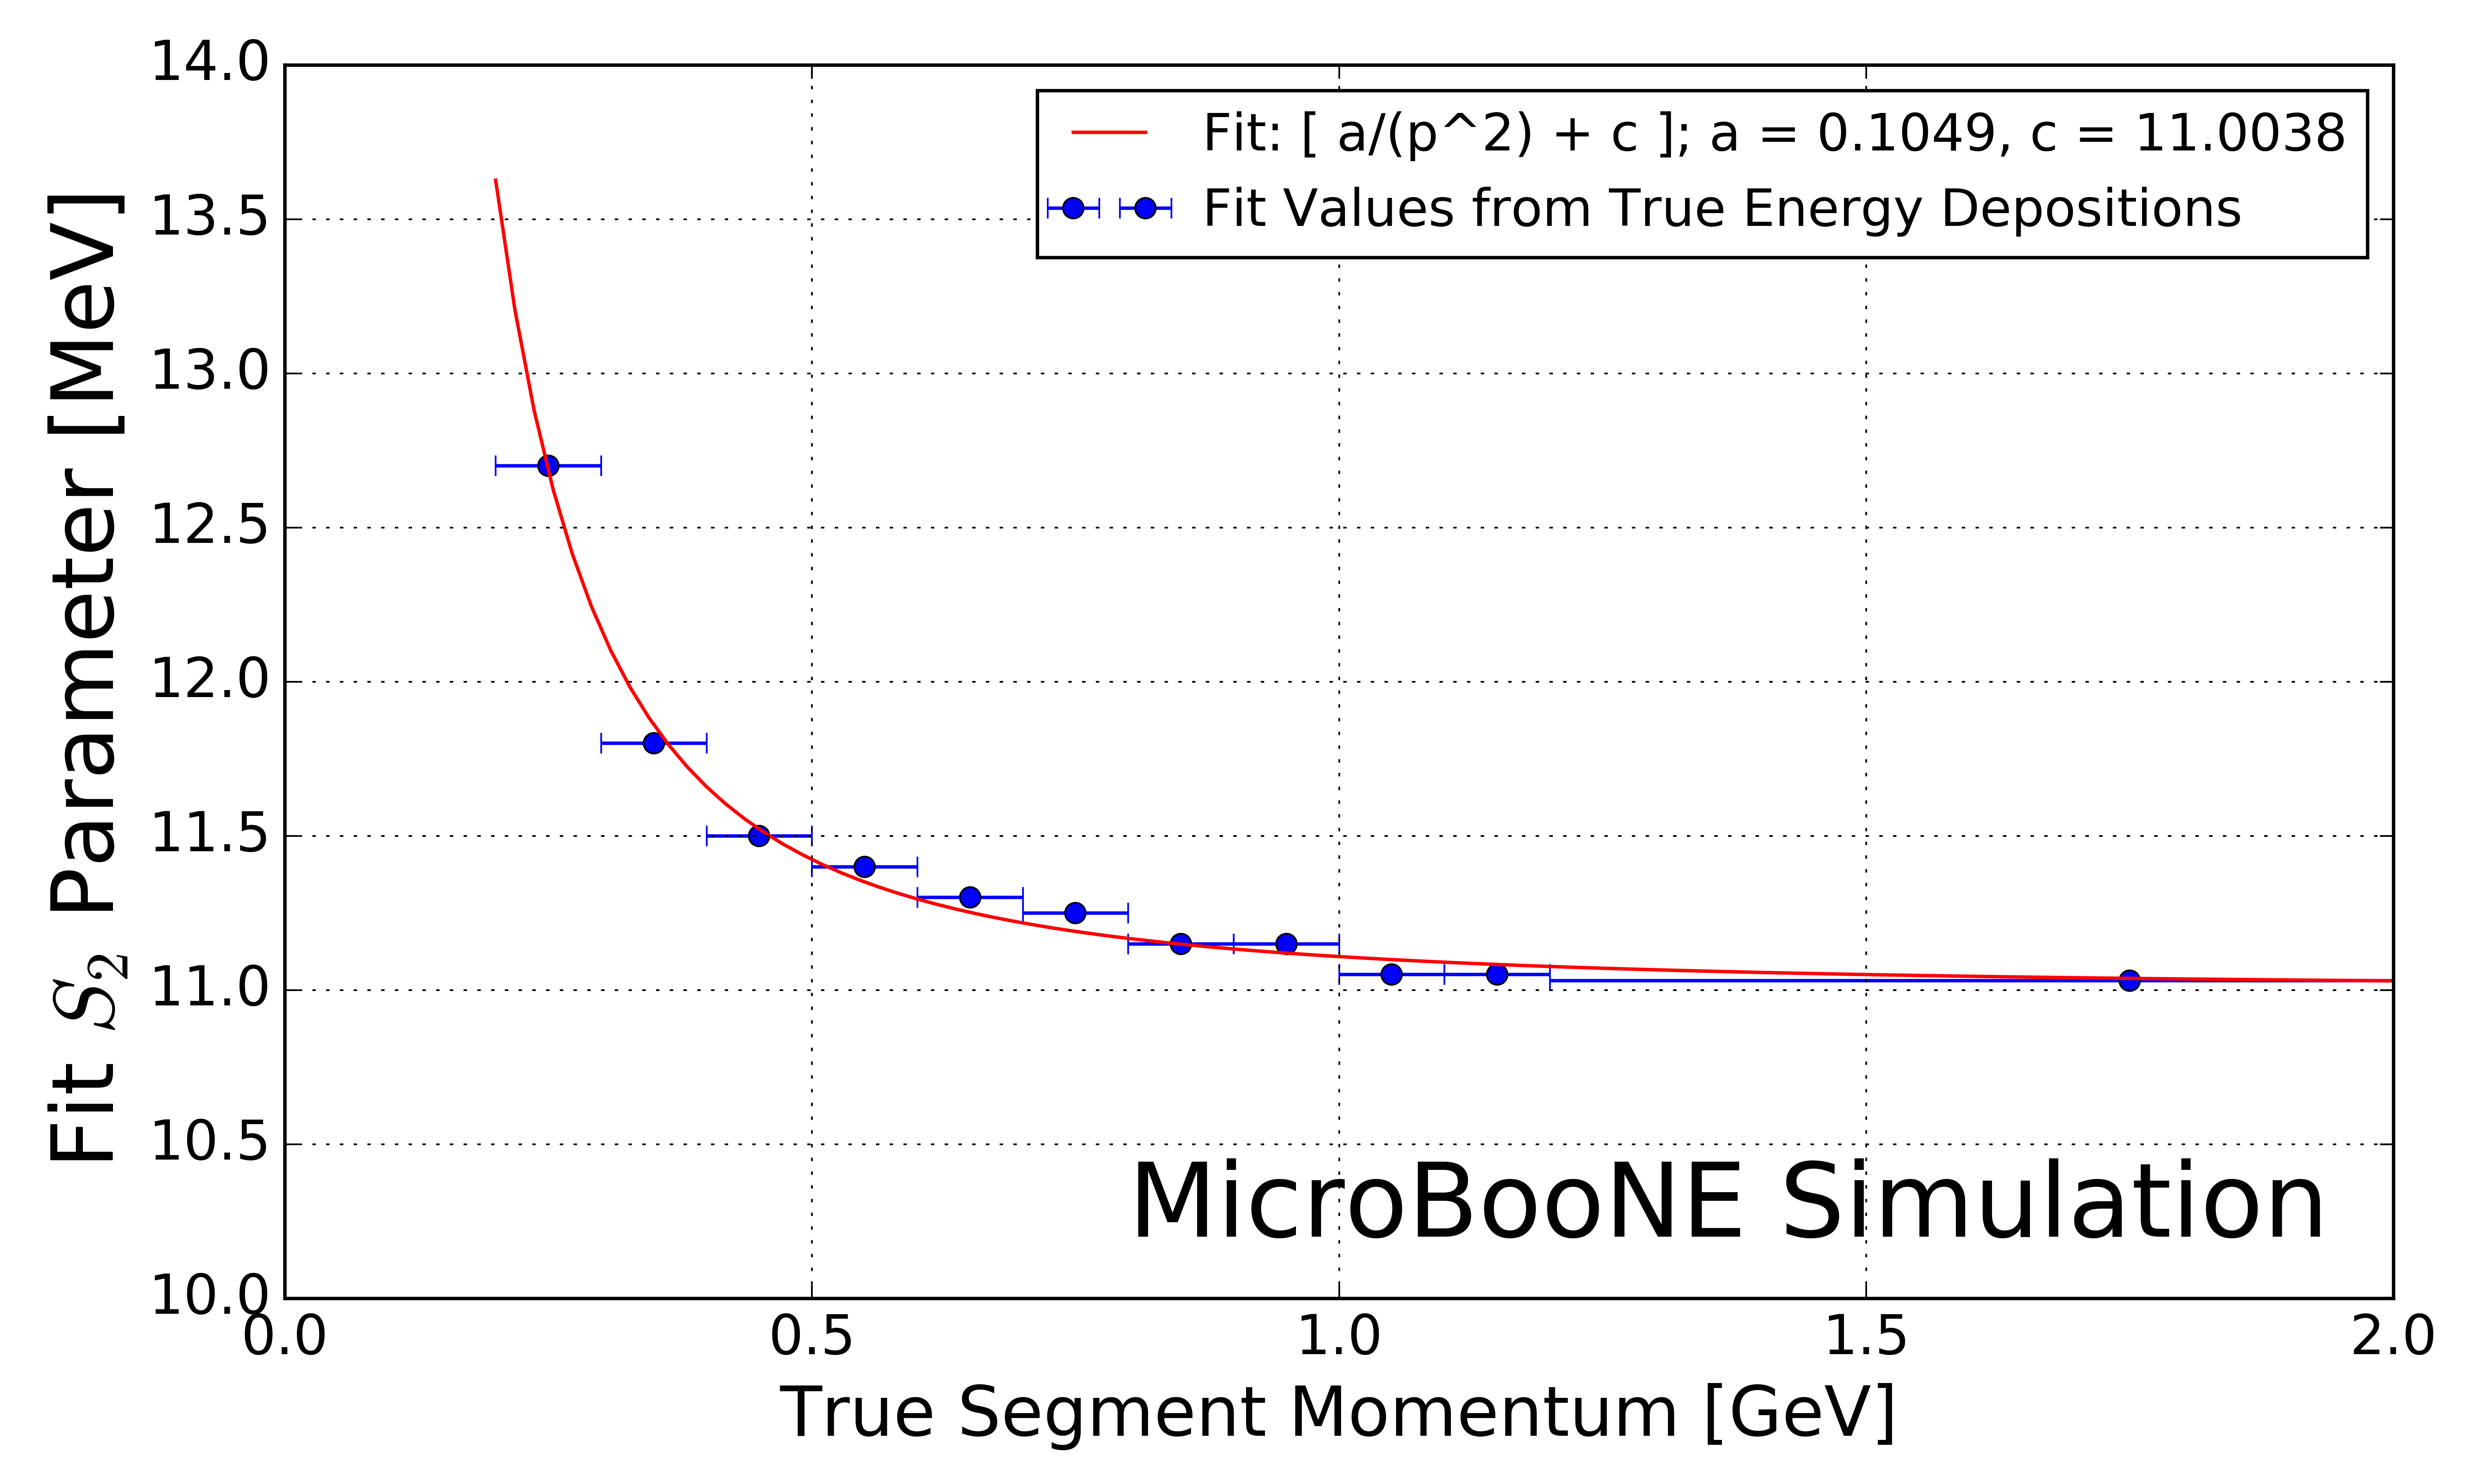
\includegraphics[width=0.9\textwidth]{Figures/MCS_PAPER_Figures/highland_constant_optimization_momentumdependent.png}
\end{center}
\caption{Fitted Highland parameter $S_2$ as a function of true segment momentum for ${\ell} = X_0$ simulated muons in the MicroBooNE LArTPC. Blue x- error bars indicate the true momentum bin width with data points drawn at the center of each bin. Shown in red is a fit to these data points with functional form $a\times p^{-2} + c$, with best fit values for parameters $a$ and $c$ shown in the legend.}
\label{retune_highland_fig1}
\end{figure}

The fitted value of $S_2$ is always less than the nominal $13.6\text{ MeV}$ for momentum greater than $0.25\text{ GeV/c}$ and asymptotically approaches a constant at higher momentum (where $\beta = 1$) of about $11.0\text{ MeV}$. The value increases in the momentum region where $\beta < 1$. Shown in red is a fit to these data points with functional form $a\times p^{-2} + c$, with best fit values for floating parameters $a$ and $c$ being $0.105~\text{MeV}^3c^{-2}$ and $11.004\text{ MeV}$ respectively. This functional form is chosen because it fits the data well, and asymptotically approaches a constant value when $\beta$ approaches 1. This function, used as a replacement for the $S_2$ parameter in the Highland formula, will henceforth be referred to as $\kappa(p)$:
\begin{equation}\label{kappa_equation}
\kappa(p) = \frac{0.105}{p^2}\text{ MeV}^3c^{-2} + 11.004\text{ MeV}.
\end{equation}

To visualize the Highland formula for ${\ell} = X_0$ both before and after the $\kappa(p)$ replacement, see figure \ref{retune_highland_fig2}. It is recommended that future LArTPC experiments use this parameterization of the Highland formula, or at the very least conduct their own studies to tune the Highland formula for scattering in argon. This formulation can also be checked in LAr-based test-beam experiments like LArIAT \cite{LARIAT_citation}.\\

\begin{figure}[ht!]
\begin{center}
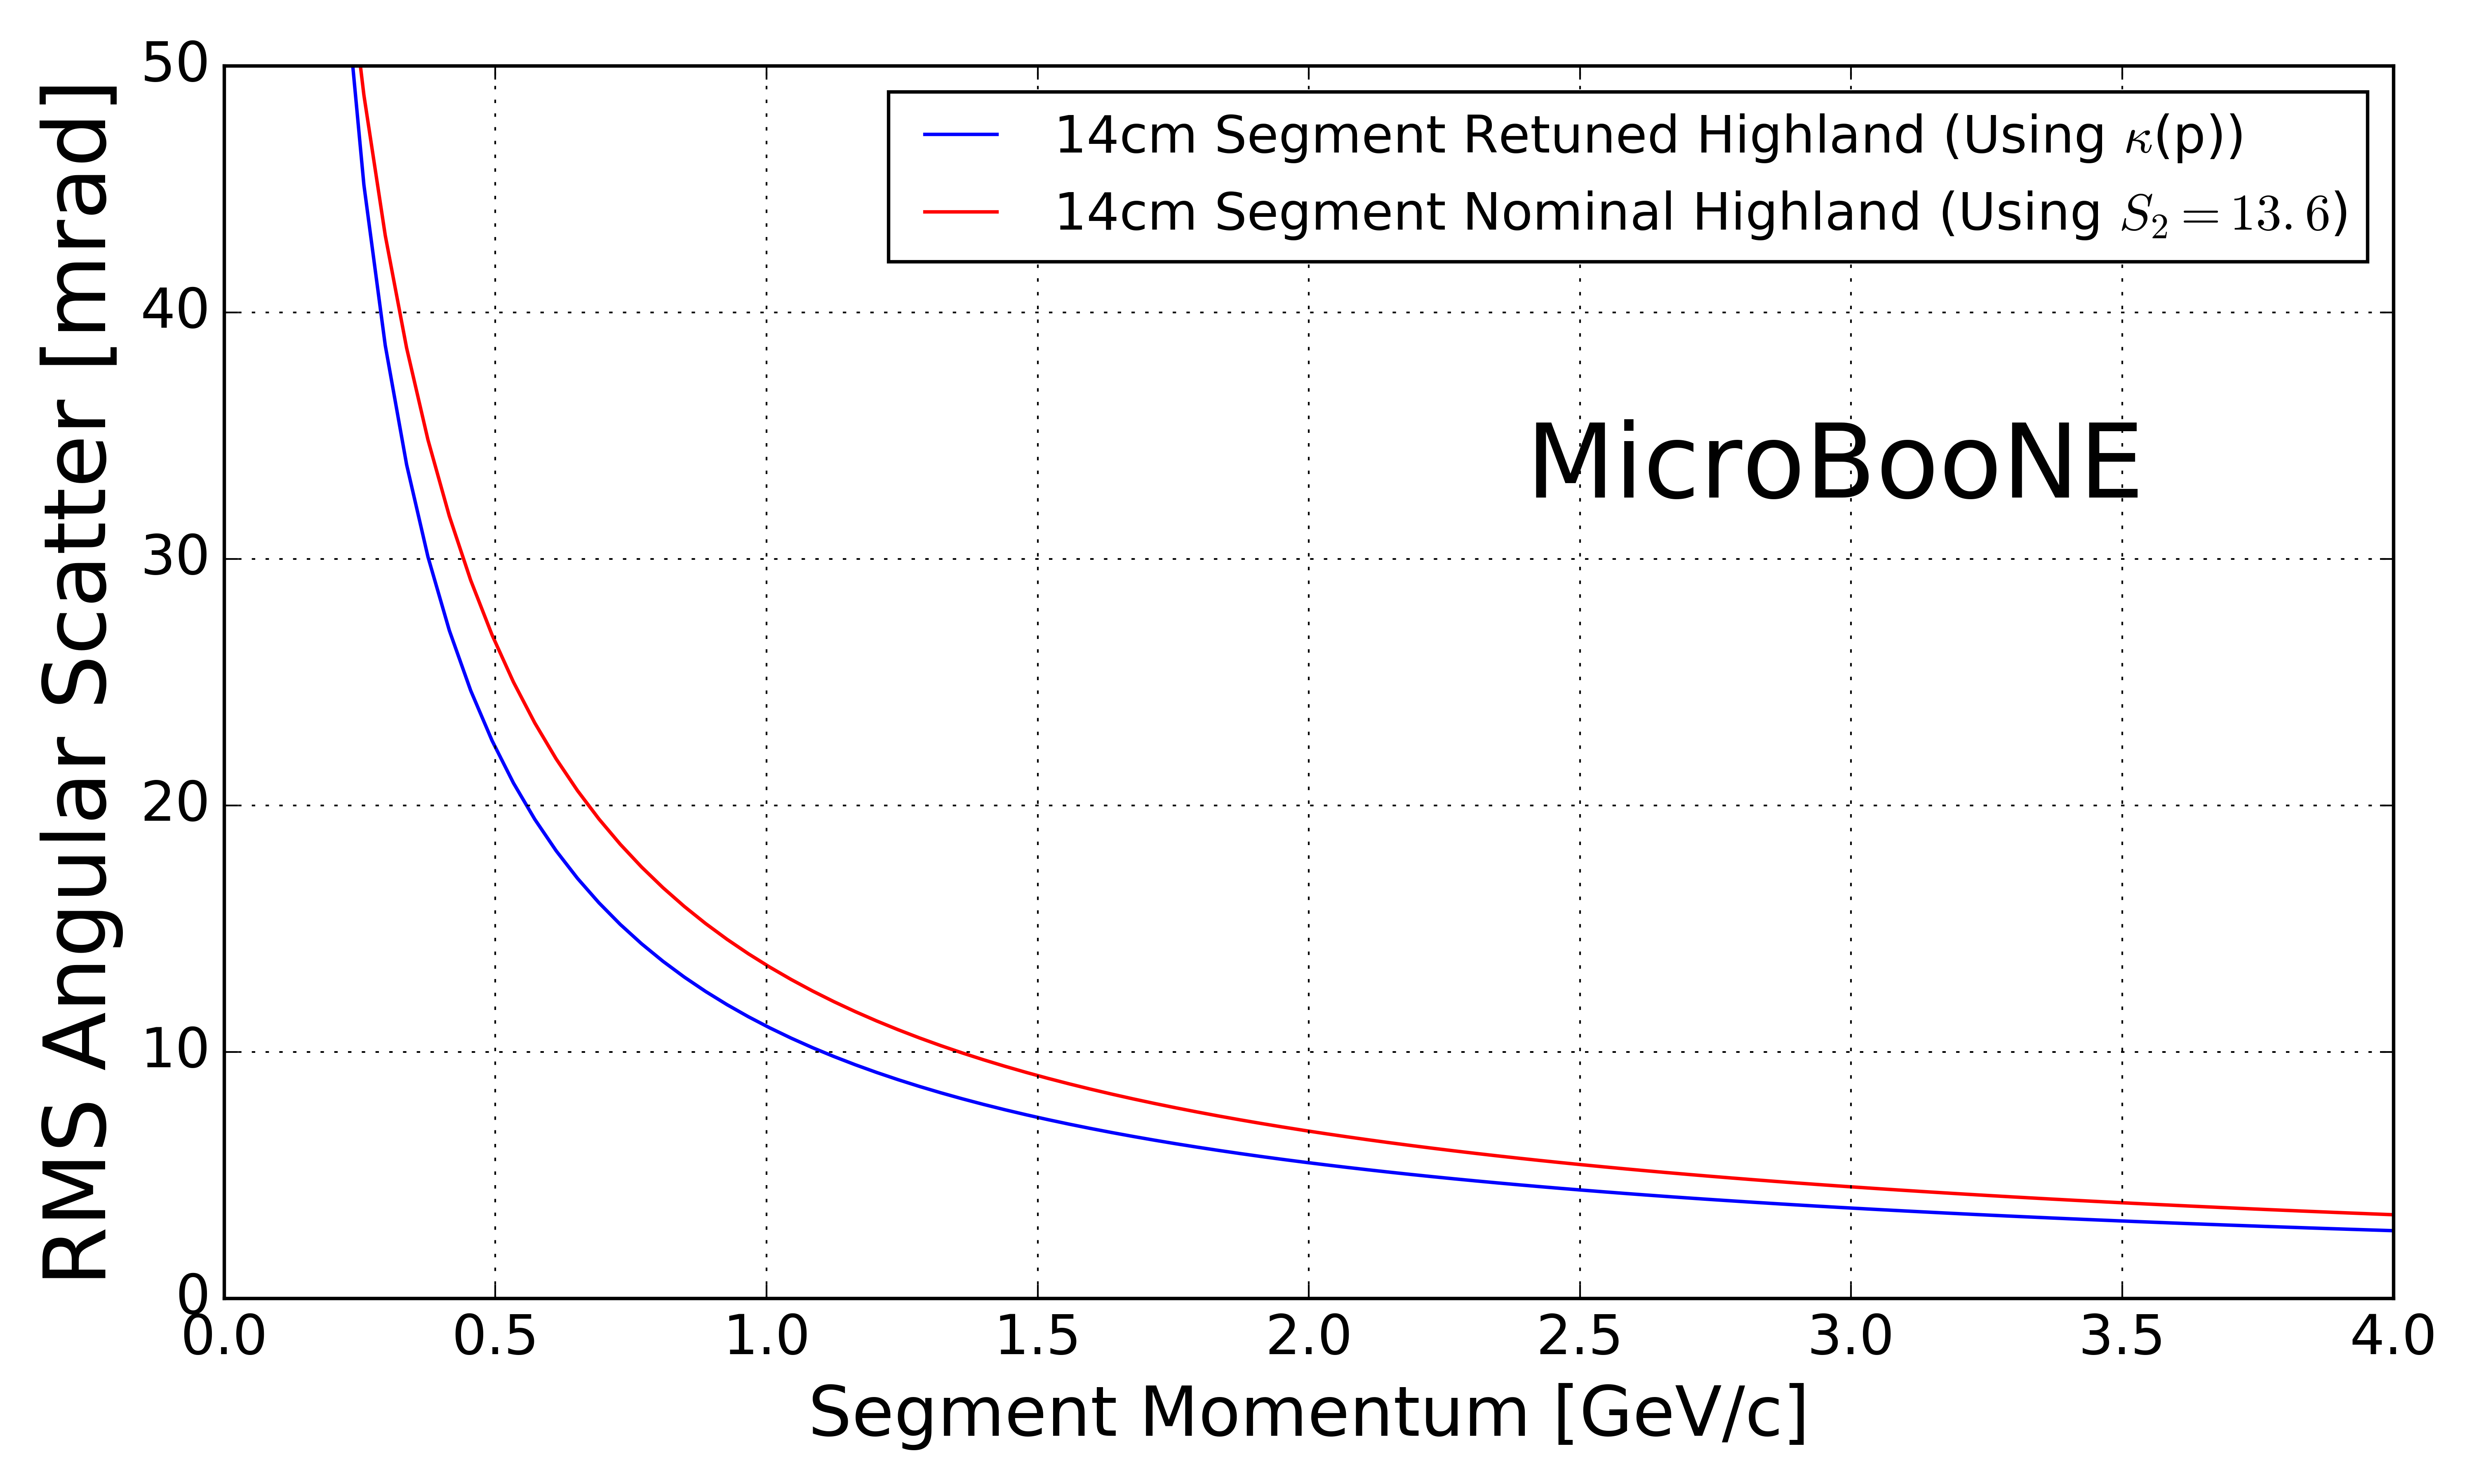
\includegraphics[width=0.9\textwidth]{Figures/MCS_PAPER_Figures/highland_formula_visualized_twoforms.png}
\end{center}
\caption{The Highland scattering RMS $\sigma_o^{\text{HL}}$ for 14 cm segment lengths and 0 detector-inherent angular resolution as a function of true momentum before and after tuning. In red is shown equation \ref{highland_simplified} (the nominal Highland formula using $S_2 = 13.6~\text{MeV}$) and in blue is the retuned Highland formula (replacing $S_2$ with $\kappa(p)$).}
\label{retune_highland_fig2}
\end{figure}

With ${\ell} = X_0$, the form of the Highland equation used in this analysis is therefore
\begin{equation}\label{modified_highland_eqtn_kappa}
\sigma_{o}^{\text{RMS}} = \sqrt{ (\sigma_o)^2 + (\sigma_o^{\text{res}})^2} = \sqrt{ \left(\frac{\kappa(p)}{p\beta c}\right)^2 + (\sigma_o^{\text{res}})^2 }.
\end{equation}


\section{MCS implementation using the maximum likelihood method}\label{MCS_technique_section}

This section explains in detail how the phenomenon of multiple Coulomb scattering is used to determine the momentum of a muon track reconstructed in a LArTPC. In general, the approach is as follows:
\begin{enumerate}
\item The three-dimensional track is divided into segments of configurable length.
\item The scattering angles between consecutive segments are measured.
\item Those angles combined with the modified, tuned Highland formula (equation \ref{modified_highland_eqtn_kappa}) are used to build a likelihood that the particle has a specific momentum, taking into account energy loss in upstream segments of the track.
\item The momentum corresponding to the maximum of the likelihood is chosen to be the MCS-computed momentum.
\end{enumerate}
Each of these steps is discussed in detail in the following subsections.\\


\subsection{Track segmentation and scattering angle computation}\label{track_segmentation_and_scattering_angle_computation_section}
 
Track segmentation refers to the subdivision of three-dimensional reconstructed trajectory points of a reconstructed track into portions of definite length. In this analysis, the tracks are automatically reconstructed by the ``pandoraNuPMA" projection matching algorithm \cite{Marshall:2015rfa}. The algorithm constructs the three-dimensional trajectory points by combining two-dimensional hits reconstructed from signals on the different wire planes along with timing information from the photomultiplier tubes. The segmentation process begins at the start of the track, and iterates through the trajectory points in order, defining segment start and stop points based on the straight-line distance between them. There is no overlap between segments. Given the subset of the three-dimensional trajectory points that corresponds to one segment of the track, a three-dimensional linear fit is applied to the data points, weighting all trajectory points equally in the fit. In this analysis, a segment length of 14 cm is used, which is a tunable parameter that has been chosen as described in the derivation of $\kappa(p)$ (equation \ref{kappa_equation}).\\

With the segments defined, the scattering angles between the linear fits from adjacent segments are computed. A coordinate transformation is performed such that the $z'$ direction is oriented along the direction of the linear fit to the first of the segment pair. The $x'$ and $y'$ coordinates are chosen such that all of $x'$, $y'$, and $z'$ are mutually orthogonal and right-handed, as shown in figure \ref{mcs_nocap_fig}. The scattering angles with respect to the $x'$ direction and the $y'$ direction are computed as input to the MCS algorithm. Only the scattering angle with respect to the $x'$ direction is drawn in figure \ref{mcs_nocap_fig}.




\subsection{Maximum likelihood theory}\label{likelihood_theory_section}

The normal probability distribution for a scattering angle in either the $x'$ or $y'$ direction, $\Delta\theta$, with an expected Gaussian uncertainty $\sigma_o$ and mean of zero is given by
\begin{equation}
f_X(\Delta\theta) = (2\pi\sigma_o^2)^{-\frac{1}{2}}\exp\left[-\frac{1}{2}\left(\frac{\Delta\theta}{\sigma_o}\right)^2\right].
\end{equation}

Here, $\sigma_o$ is the RMS angular deflection computed by the modified, tuned Highland formula (equation \ref{modified_highland_eqtn_kappa}), which is a function of the momentum and the length of that segment. Since energy is lost between segments along the track, $\sigma_o$ increases for each angular measurement along the track. We therefore replace $\sigma_o$ with $\sigma_{o,j}$, where $j$ is an index representative of the segment. \newline

To obtain the likelihood, we take the product of $f_X(\Delta\theta_j)$ over all $n$ of the $\Delta\theta_j$ segment-to-segment scatters along the track. This product can be written as
\begin{equation}
L(\sigma_{o,1},...,\sigma_{o,n};\Delta\theta_1,...,\Delta\theta_n) = (2\pi)^{-\frac{n}{2}}\times\prod_{j=1}^{n}(\sigma_{o,j})^{-1} \times \exp\left[-\frac{1}{2}\sum_{j=1}^{n}\left(\frac{\Delta\theta_j}{\sigma_{o,j}}\right)^2\right].
\end{equation}

Rather than maximizing the likelihood it is more computationally convenient to instead minimize the negative log likelihood. Inverting the sign and taking $\ln(L)$ gives an expression that is related to a $\chi^2$ variable:
\begin{equation}\label{leo_llhd_eqtn}
-l(\mu_o;\sigma_{o,1},...,\sigma_{o,n};\Delta\theta_1,...,\Delta\theta_n) = -\ln(L) = \frac{n}{2}\ln(2\pi) + \sum_{j=1}^{n}\ln(\sigma_{o,j}) + \frac{1}{2}\sum_{j=1}^{n}\left(\frac{\Delta\theta_j}{\sigma_{o,j}}\right)^2
\end{equation}



\subsection{Maximum likelihood implementation}\label{maximum_likelihood_section}

Given a set of angular deflections in the $x'$ and $y'$ directions for each segment as described in section \ref{track_segmentation_and_scattering_angle_computation_section} a scan is done over the postulated initial energy, $E_t$, in steps of 1 MeV up to 7.5 GeV. The step with the smallest negative log likelihood (equation \ref{leo_llhd_eqtn}) is chosen as the MCS energy. Equation \ref{leo_llhd_eqtn} includes a $\sigma_{o,j}$ term that changes for consecutive segments because their associated energy is decreasing. The energy of the $j$th segment is related to $E_t$ by

\begin{equation}\label{segment_E_equation}
E_{j} = E_t - \Delta E_{j},
\end{equation}

\noindent where $\Delta E_{j}$ is the energy loss upstream of this segment, computed by integrating the muon stopping power curve given by the Bethe-Bloch equation described by the Particle Data Group (PDG) \cite{stoppingpowersource} along the length of track upstream of this segment. Equation \ref{segment_E_equation} introduces a minimum allowable track energy determined by the length of the track, as $E_{j}$ must remain positive. This value of segment energy is converted to a momentum $p$ with the relativistic energy-momentum relation assuming the muon mass, and is then used to predict the RMS angular scatter for that segment ($\sigma_o$) by way of equation \ref{modified_highland_eqtn_kappa}. 

\section{Range-based energy validation from simulation}\label{Range_Energy_Validation_section}
In order to quantify the performance of the MCS energy estimation method on fully contained muons in data, an independent determination of energy is needed. Range-based energy, $E_{\text{range}}$ is used here because the true energy $E_{\text{true}}$ will not be known in analyzing detector data. The stopping power of muons in liquid argon is well described by the continuous slowing-down approximation (CSDA) by the particle data group, and agrees with data at the sub-percent level \cite{MIPenergysource} \cite{PDG_spline_table} \cite{NISTdata}. By using a linear interpolation between points in the stopping power table of ref. \cite{PDG_spline_table}, the length of a track can be used to reconstruct the muon's total energy with good accuracy. A simulated sample of fully contained BNB neutrino-induced muons longer than one meter is used to quantify the bias and resolution for the range-based energy estimation technique. The range is defined as the straight-line distance between the true starting point and true stopping point of a muon, even though the trajectories are not perfectly straight lines. The bias and resolution are computed in bins of true total energy of the muons by fitting a Gaussian function to a distribution of the fractional energy difference $(E_{\text{Range}}-E_{\text{True}})/(E_{\text{True}})$ in each bin. The mean of each Gaussian yields the bias for that true energy bin, and the width indicates the resolution. Figure \ref{true_range_bias_resolution_MCTrack_fig} shows the bias and resolution for the range-based energy reconstruction method. The bias is negligible and the resolution for this method of energy reconstruction increases slightly with true muon energy but remains on the order of (2-4)\%. This result demonstrates that range-based energy (and therefore range-based momentum) is a good estimator of the true energy (momentum) of a reconstructed contained muon track in data, assuming that the track is well reconstructed in terms of length.

\begin{figure}
\centering
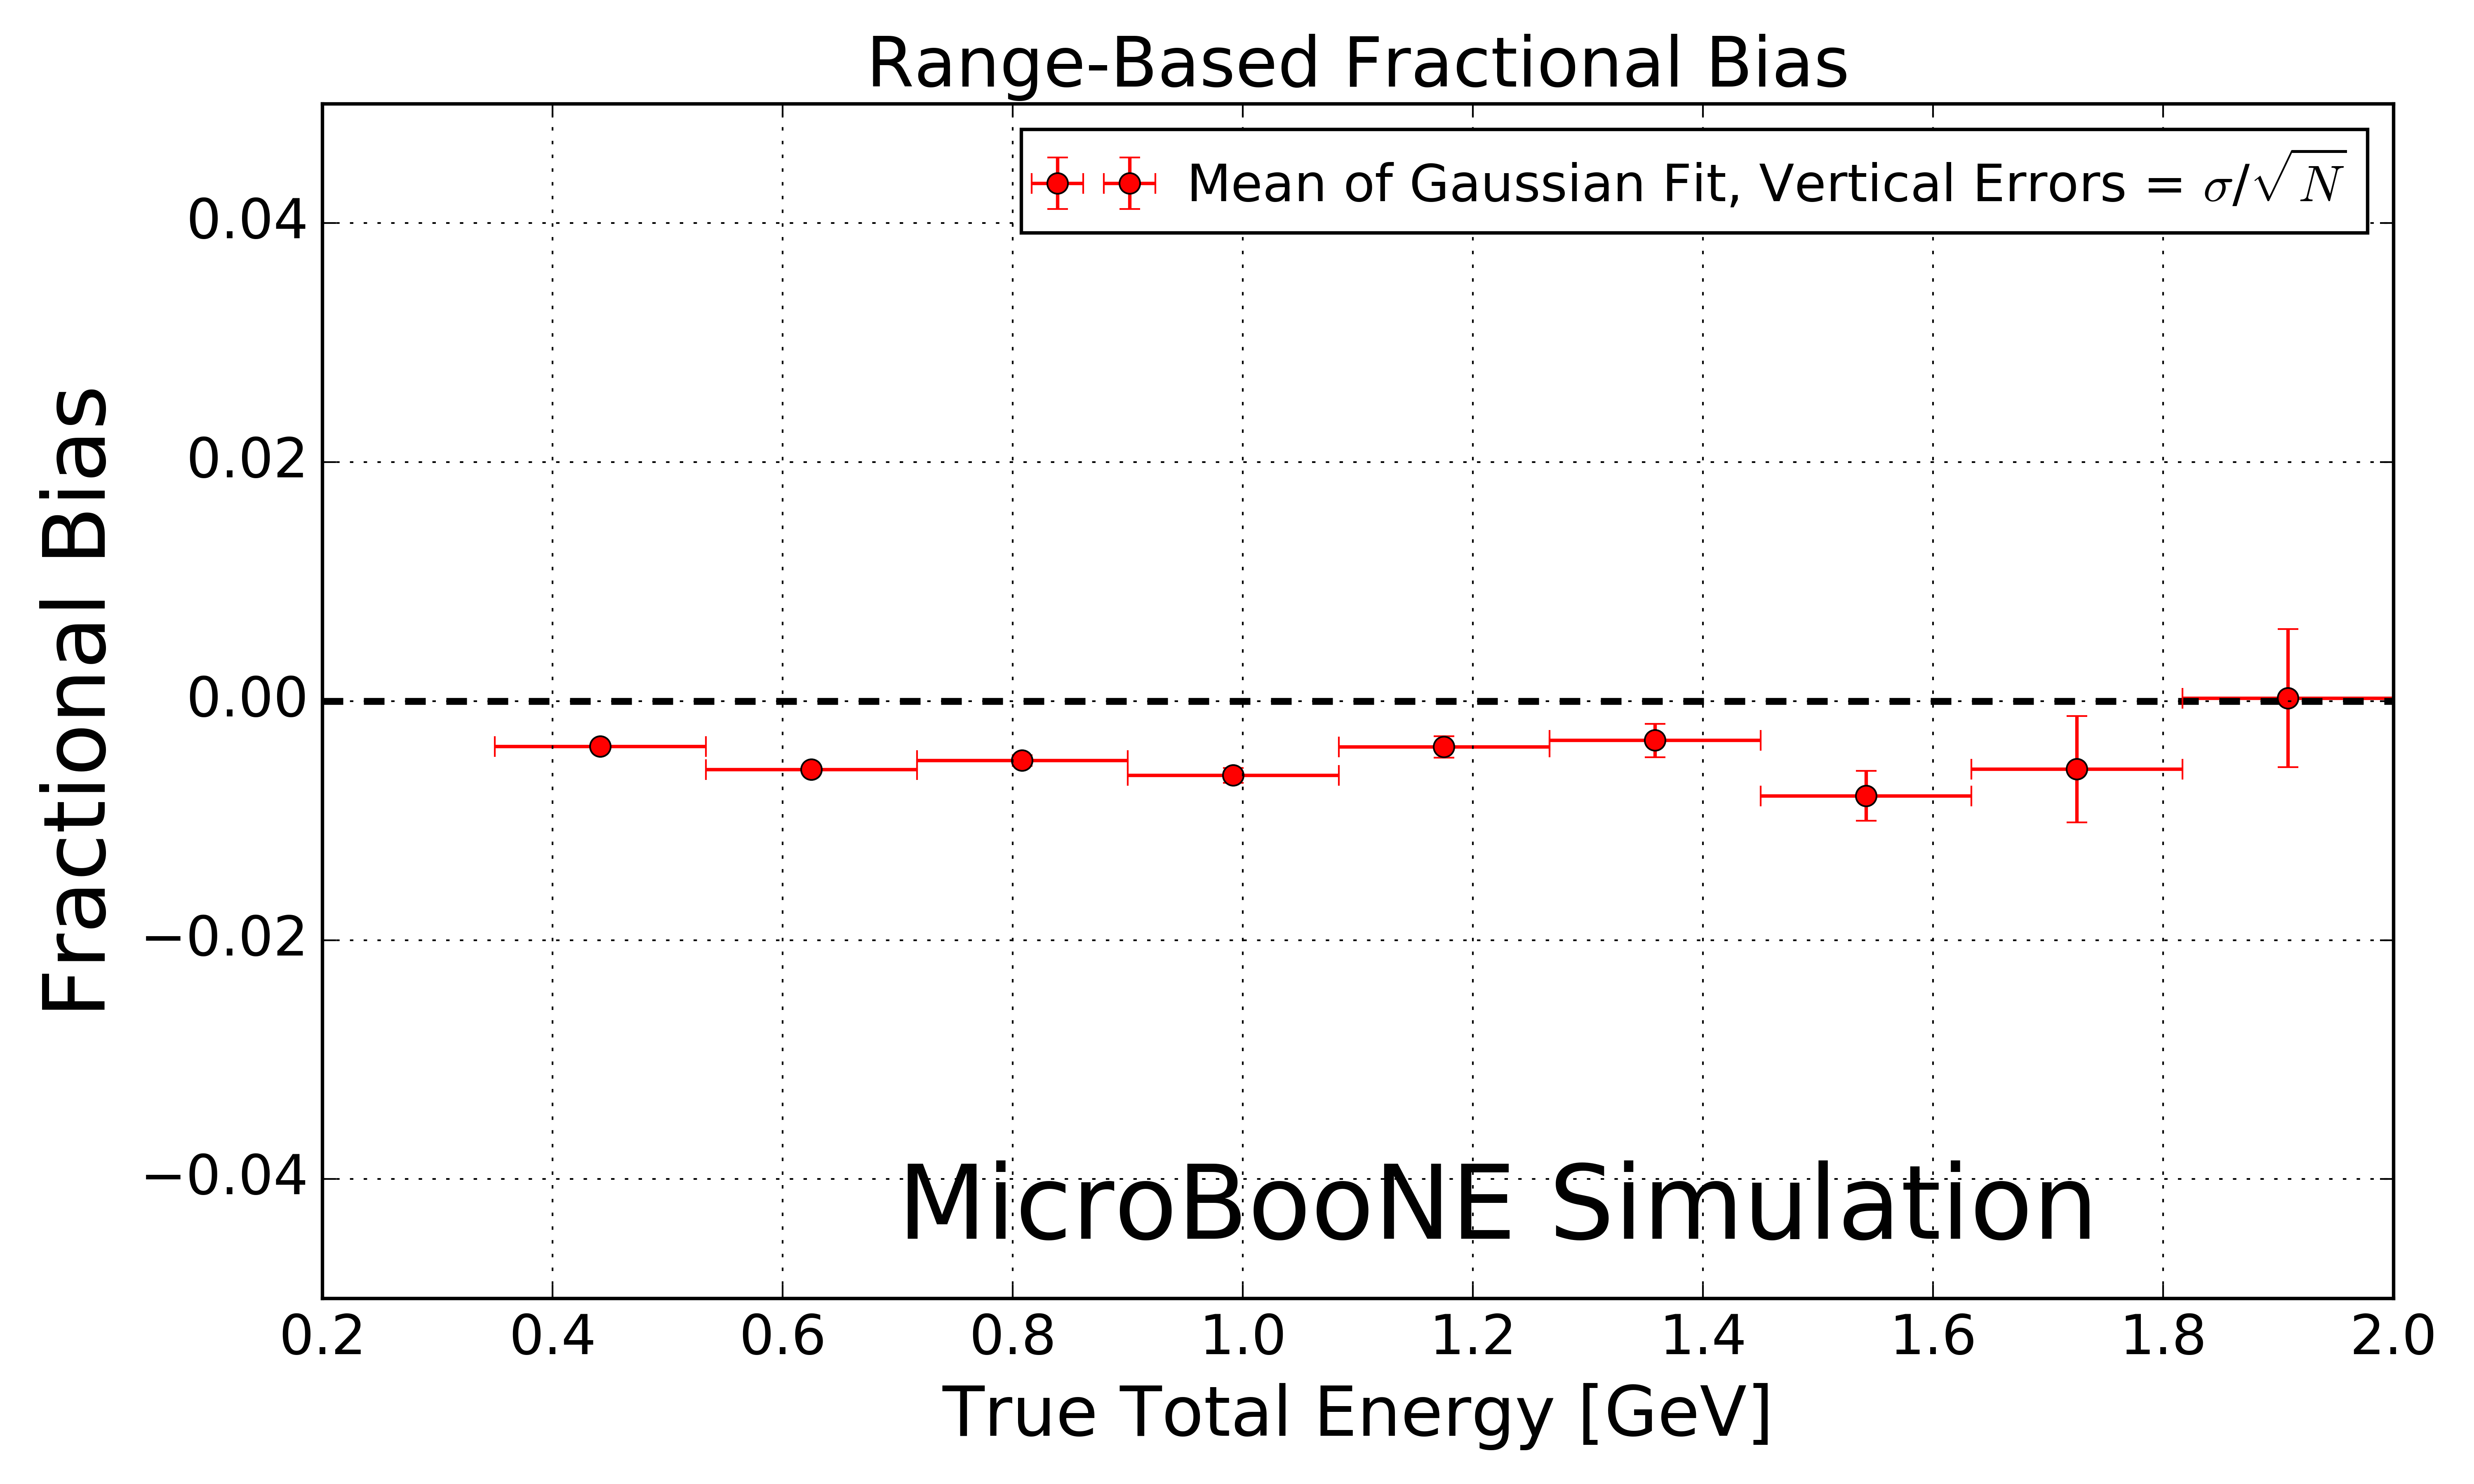
\includegraphics[width=0.9\textwidth]
	{Figures/MCS_PAPER_Figures/true_range_bias_MCBNBMCTrack.png}
\includegraphics[width=0.9\textwidth]
	{Figures/MCS_PAPER_Figures/true_range_resolution_MCBNBMCTrack.png}
\caption{Range-based energy fractional bias (a) and resolution (b) from a sample of simulated fully contained BNB neutrino-induced muons using true starting and stopping positions of the track. The bias is less than 1\% and the resolution is below $\approx$4\%.}
\label{true_range_bias_resolution_MCTrack_fig}
\end{figure}






\section{MCS performance on beam neutrino-induced muons in MicroBooNE data}\label{data_performance_section}

\subsection{Input sample}\label{input_sample_section}
This part of the analysis is based on triggered neutrino interaction events in MicroBooNE corresponding to $\approx 5 \times 10^{19}$ protons on target, which is a small subset ($<$10\%) of the nominal protons on target scheduled to be delivered to the detector. These events are run through a fully automated reconstruction chain that produces reconstructed objects including three-dimensional neutrino interaction points (vertices), three-dimensional tracks (as described in section \ref{track_segmentation_and_scattering_angle_computation_section}) for each outgoing secondary particle from the interaction, and PMT-reconstructed optical flashes from the interaction scintillation light. The fiducial volume used in this analysis is defined in section \ref{sec:intro}.

\subsection{Event selection}
The following selection criteria are placed on the reconstructed objects to select $\nu_\mu$ charged-current interactions in which a candidate muon track exiting the interaction vertex is fully contained within the fiducial volume:
\begin{enumerate}
\item The event must have at least one bright optical flash, reconstructed from PMT timing signals, in coincidence with the expected BNB-neutrino arrival time.
\item Two or more reconstructed tracks must originate from the same reconstructed vertex within the fiducial volume.
\item The $z$ coordinate of the optical flash, as determined by the pulse height and timing of signals in the 32 PMTs, must be within 70 cm of any point on the $z$ projection of the candidate muon track.
\item For events with exactly two tracks originating from the vertex, additional calorimetric criteria are applied to mitigate backgrounds from cosmic muons that arrive in time with the passage of the beam, then stop and decay to an electron that is reconstructed as a track.
\item The longest track originating from the vertex is assumed to be a muon, and it must be fully contained within the fiducial volume.
\item The length of the longest track must be $>$1~m in order to have sufficient sampling points in the MCS likelihood to obtain a reasonable estimate of momentum.
\end{enumerate}

These selection criteria are chosen to select a sample of tracks with high purity. In this sample of MicroBooNE data, 598 events (tracks) remain after all selections. The low statistics in this sample is due to the size of the input sample and the low efficiency associated with the applied high-purity selection, described in section \ref{input_sample_section}. Each of these events (tracks) was scanned by hand with a 2D interactive event display showing the raw wire signals of the interaction from each wire plane, with the 2D projection of the reconstructed muon track and vertex overlaid. The scanning was done to ensure the track is well reconstructed with start point close to the reconstructed vertex and end point close to the end of the visible wire-signal track in all three planes. During the scanning, obvious mis-identification topologies were removed. An example of such a topology is a stopping cosmic-ray muon decaying into an electron. After rejecting events (tracks) based on hand scanning, 396 tracks remain for analysis.


\subsection{Validation of the Highland formula}\label{highland_validation_section}
The Highland formula indicates that distributions of angular deviations of the track, segment by segment, in both the $x'$ and $y'$ directions divided by the width predicted from the Highland equation $\sigma_o^{\text{RMS}}$ (equation \ref{modified_highland_eqtn_kappa}) should be Gaussian with a width of unity. In order to calculate the momentum $p$ in the Highland equation, $p$ for each segment is computed with equation \ref{segment_E_equation}, where $E_t$ comes from the converged MCS-computed momentum of the track. For each consecutive pair of segments in this sample of 396 tracks, the angular scatter divided by the Highland expected RMS (including detector resolution term, $\sigma_o^{\text{res}}$) is an entry in the area-normalized distribution shown in figure \ref{Highland_validation_fig}. These 396 tracks have on average 12 segments each, therefore this histogram has approximately $396\times12\times2=9504$ entries. The additional factor of 2 comes from angular scatters both in the $x'$ and $y'$ directions. The distribution has an RMS of unity, thus validating the MCS technique used in this analysis.

\begin{figure}[ht!]
\centering
	\includegraphics[width=0.9\textwidth]{Figures/MCS_PAPER_Figures/Highland_validation_DataBNBSelectedRecoTrack_goodscan.png} \\
\caption{Segment-to-segment measured angular scatters in both the $x'$ and $y'$ directions divided by the width $\sigma_o^{\text{RMS}}$ predicted by the Highland formula (equation \ref{highland_eqtn}) for the automatically selected beam neutrino-induced fully contained muon sample in MicroBooNE data after hand scanning to remove poorly reconstructed tracks and obvious mis-identification topologies.}\label{Highland_validation_fig}
\end{figure}


\subsection{MCS momentum validation}\label{MCS_Momentum_Validation_DataRecoTrack_section}

MCS momentum versus range-based momentum for this sample of 396 tracks is shown in figure \ref{realdata_goodhandscan_fig}. The fractional bias and resolution as a function of range-based momentum for this sample is shown in figure \ref{MCS_range_bias_resolution_DataRecoTrack_fig}. In order to compute this bias and resolution, distributions of fractional inverse momentum difference $(p_{\text{MCS}}^{-1} - p_{\text{Range}}^{-1})/(p_{\text{Range}}^{-1})$ in bins of range-based momentum $p_{\text{Range}}$ are fit to Gaussian functions, where the mean of the fit determines the bias while the width of the fit determines the resolution for that bin. Inverse momentum is used here because the binned distributions are more Gaussian since the Highland formula measures inverse momentum in terms of track angles that have reasonably Gaussian errors. Simply using the mean and RMS of the binned distributions yields similar results. Also shown in this figure are the bias and resolutions for a simulated sample consisting of a full BNB simulation with CORSIKA-generated \cite{corsika_ref} cosmic overlays passed through an identical reconstruction and event selection chain. Rather than hand scanning this sample, true simulation information is used by requiring the longest reconstructed track to be matched well to the true starting and stopping point of the $\nu_\mu$CC muon. This removes any mis-identifications or interference from the simulated cosmics. 


\begin{figure}[ht!]
\centering
	\includegraphics[width=0.9\textwidth]{Figures/MCS_PAPER_Figures/MCS_range_momentum_DataRecoTracks_goodhandscan.png} \\
\caption{MCS-computed momentum versus range momentum for the automatically selected beam neutrino-induced fully contained muon sample in MicroBooNE data after hand scanning to remove poorly reconstructed tracks and obvious mis-identification topologies. The color (z) scale indicates number of tracks.}\label{realdata_goodhandscan_fig}
\end{figure}



\begin{figure}
\centering
	\includegraphics[width=0.9\textwidth]{Figures/MCS_PAPER_Figures/MCS_range_bias_multiplesamples_publicplot.png}
	\includegraphics[width=0.9\textwidth]{Figures/MCS_PAPER_Figures/MCS_range_resolution_multiplesamples_publicplot.png}
\caption{Inverse momentum difference (as defined in the text) fractional bias (top) and resolution (bottom) for automatically selected contained $\nu_\mu$CC-induced muons from full simulated BNB events with cosmic overlay where the track matches with the true muon track (blue), and automatically selected and hand-scanned (see text) contained $\nu_\mu$CC-induced muons from MicroBooNE data (green).}\label{MCS_range_bias_resolution_DataRecoTrack_fig}
\end{figure}

Figure \ref{MCS_range_bias_resolution_DataRecoTrack_fig} indicates a bias in the MCS momentum calculation on the order of a few percent, with a resolution that decreases from about 10\% for contained reconstructed tracks in data and simulation with range momentum around 0.45 GeV/c (which corresponds to a length of about 1.5 m) to below 5\% for contained reconstructed tracks in data and simulation with range momentum about 1.15 GeV/c (which corresponds to a length of about 4.6 meters). Resolution improving with length of track is expected; the longer the track, the more angular scattering measurements can be made to improve the likelihood. In general the bias and resolutions agree between data and simulation within uncertainty.\\

\subsection{Impact of Highland formula tuning}\label{highland_formula_tuning_impact_section}

In order to examine the impact of the Highland formula tuning described in section \ref{highland_tuning_section}, the fractional bias and resolution on the simulated sample of contained muons described in section \ref{MCS_Momentum_Validation_DataRecoTrack_section} both with the nominal Highland formula (equation \ref{modified_highland_eqtn}) and with the retuned Highland formula (equation \ref{modified_highland_eqtn_kappa}) are shown in figure \ref{MCS_range_bias_resolution_compareHighlandFormulas_fig}. Tuning the Highland formula improves the magnitude of the fractional bias to below 2\%, and improves the fractional resolution by (2-3)\%, with the most improvement at the lowest momenta.

\begin{figure}
\centering
	\includegraphics[width=0.9\textwidth]{Figures/MCS_PAPER_Figures/MCS_range_bias_compareHighlandTuning_publicplot.png}
	\includegraphics[width=0.9\textwidth]{Figures/MCS_PAPER_Figures/MCS_range_resolution_compareHighlandTuning_publicplot.png}
\caption{Inverse momentum difference (as defined in the text) fractional bias (top) and resolution (bottom) for automatically selected contained $\nu_\mu$CC-induced muons from full simulated BNB events with cosmic overlay where the track matches with the true muon track both using the nominal Highland formula (equation \ref{modified_highland_eqtn}) (red) and the retuned Highland formula (equation \ref{modified_highland_eqtn_kappa}) (blue).}\label{MCS_range_bias_resolution_compareHighlandFormulas_fig}
\end{figure}






\section{MCS performance on exiting muons in MicroBooNE simulation}
In this section we quantify the MCS algorithm performance on a sample of well reconstructed exiting muon tracks in simulated BNB $\nu_\mu$CC interactions within the MicroBooNE detector. The tracks are automatically reconstructed by the same ``pandoraNuPMA'' algorithm described in section \ref{track_segmentation_and_scattering_angle_computation_section}, and all tracks have a length of at least $1$~m within the TPC. This simulation does not include space-charge effects. The relationship between the MCS and the true momenta at the beginning of the track as given by simulation for this sample of 28,000 exiting muon tracks is shown in figure \ref{MCS_true_comparison_exiting_fig}.\\

\begin{figure}[ht!]
\centering
	\includegraphics[width=0.9\textwidth]{Figures/MCS_PAPER_Figures/MCS_true_comparison_MCBNBRecoTrackExiting.png} \\
\caption{MCS-computed momentum versus true momentum for the sample of simulated exiting BNB $\nu_\mu$CC muons in MicroBooNE with at least one meter of track contained within the TPC. The color (z) scale indicates number of tracks.}\label{MCS_true_comparison_exiting_fig}
\end{figure}

The distribution of $(p_{\text{MCS}}^{-1} - p_{\text{true}}^{-1})/(p_{\text{true}}^{-1})$ is shown for four representative bins of true momentum in figure \ref{MCS_true_exiting_resolution_MCBNBRecoTrackExiting_slices_fig}, along with the Gaussian fit to each distribution. Low-momentum tails where the MCS momentum is underestimated due to poor track reconstruction lie outside the fitted Gaussian function.\\

The fractional bias and resolution as a function of true momentum are shown in figure \ref{exitingRecoTrack_bias_resolution_fig_alllengths}. The bias is below 4\% for all momenta, and the resolution is $\approx$ 14\% in the relevant momentum region for BNB $\nu_\mu$CC muons (below 2 GeV/c). The resolution worsens for muon momenta above this region because the angular scatters begin to be comparable with the detector resolution term of 3 mrad. The resolution improves for longer lengths of track contained, with 10\% resolution for muons with $p<2$~$\text{GeV/c}$ with more than 3.5 meters contained. The mean length of track contained for muons in this analysis is 212 cm.\\


\begin{figure}
\centering
\includegraphics[width=0.45\textwidth]
	{Figures/MCS_PAPER_Figures/{MCS_true_exiting_resolution_MCBNBRecoTrackExiting_slice_0.35_0.76}.png}
\includegraphics[width=0.45\textwidth]
	{Figures/MCS_PAPER_Figures/{MCS_true_exiting_resolution_MCBNBRecoTrackExiting_slice_1.97_2.38}.png}
\includegraphics[width=0.45\textwidth]
	{Figures/MCS_PAPER_Figures/{MCS_true_exiting_resolution_MCBNBRecoTrackExiting_slice_2.78_3.19}.png}
\includegraphics[width=0.45\textwidth]
	{Figures/MCS_PAPER_Figures/{MCS_true_exiting_resolution_MCBNBRecoTrackExiting_slice_3.59_4.00}.png}
\caption{Fractional momentum difference for a few representative bins of true momentum for a sample of simulated exiting muon tracks. The y-axis is number of tracks, and the x-axis is $(p_{\text{MCS}}^{-1} - p_{\text{true}}^{-1})/(p_{\text{true}}^{-1})$.}
\label{MCS_true_exiting_resolution_MCBNBRecoTrackExiting_slices_fig}
\end{figure}

\begin{figure}
\centering
\includegraphics[width=0.9\textwidth]
	{Figures/MCS_PAPER_Figures/MCS_true_exiting_bias_MCBNBRecoTrackExiting.png}
\includegraphics[width=0.9\textwidth]
	{Figures/MCS_PAPER_Figures/MCS_true_exiting_resolution_MCBNBRecoTrackExiting.png}
\caption{MCS momentum fractional bias (top) and resolution (bottom) as a function of true momentum from a sample of exiting reconstructed muon tracks.}
\label{exitingRecoTrack_bias_resolution_fig_alllengths}
\end{figure}



\section{Conclusions}
We have described a multiple Coulomb scattering maximum likelihood method for estimating the momentum of a three dimensional reconstructed track in a LArTPC and have provided motivation for development of such a technique. Using simulation, we have shown that the standard Highland formula should be re-tuned specifically for scattering in liquid argon. After validating range-based momentum-determination techniques with MicroBooNE simulation, we have demonstrated the accuracy and precision of the MCS-based momentum reconstruction in MicroBooNE data by comparing its performance to the range-based method. For 398 fully-contained BNB $\nu_\mu$CC-induced muons, the MCS method exhibits a fractional bias below 3\% and a momentum resolution below 10\%, agreeing with simulation predictions. Using simulation of a separate sample of uncontained muon tracks in MicroBooNE with at least one meter contained in the active volume, the MCS-based reconstruction is shown to produce a fractional bias below 4\% and a momentum resolution of better than 15\% for muons in the relevant BNB energy region of below 2 GeV.

\section{Acknowledgments}
This material is based upon work supported by the following: the U.S. Department of Energy, Office of Science, Offices of High Energy Physics and Nuclear Physics; the U.S. National Science Foundation; the Swiss National Science Foundation; the Science and Technology Facilities Council of the United Kingdom; and The Royal Society (United Kingdom). Additional support for the laser calibration system and cosmic ray tagger was provided by the Albert Einstein Center for Fundamental Physics. Fermilab is operated by Fermi Research Alliance, LLC under Contract No. DE-AC02-07CH11359 with the United States Department of Energy.


\chapter{Conclusions}
\label{sec:conclusions}
Following some introductory material including a description of neutrinos and neutrino oscillations, the liquid argon time projection technique and specifically the MicroBooNE detector at the Fermi National Accelerator Lab, and the results and implications of the LSND and MiniBooNE experiments, three subsequent MicroBooNE analyses have been described. All three of these analyses are closely interconnected, and are ultimately geared towards searching for and understanding the MiniBooNE measured low energy excess of electromagnetic events in the MicroBooNE detector.\\

First, a detailed sensitivity analysis was described. It involved simulating beam neutrino events in the MicroBooNE detector, and using reconstruction algorithms to select them. These algorithms included the leveraging of 3D energy deposition ($dE/dx$) information to separate electrons from photons, a capability which MiniBooNE did not possess. Additionally, MiniBooNE low energy excess public data releases were used to simulate what the excess would look like in MicroBooNE, assuming it was induced by an excess of beam $\nu_e$ interactions. Ultimately, a sensitivity was estimated for the MicroBooNE detector to observe such a signal. The dominant background in this search was (irreducible) intrinsic $\nu_e$ from both pion and kaon decay in the beam-line, and the flux uncertainty associated with the production of these particles is large.\\

The first steps toward the analysis to measure the $K^+$ production in the beam-line by selecting high energy $\nu_\mu$ events was presented. This analysis constrains the significant portion of intrinsic $\nu_e$ backgrounds which come from kaon decay in the beam-line. This important measurement was initially done by the SciBooNE collaboration. Measuring the $K^+$ production in MicroBooNE is relevant because the MicroBooNE detector has a different neutrino target material (argon) than SciBooNE (polystyrene), and the $K^+$ production measurement can be done \textit{in situ} in the same detector searching for the low energy excess.\\

An important part of the $K^+$ analysis involves measuring the energy of muons created in $\nu_\mu$ interactions which exit the detector. While measuring the energy of fully contained muons is straightforward with calorimetric or range-based techniques, the only method to measure that of exiting tracks is by means of multiple Coulomb scattering (MCS). A detailed investigation into how the MCS algorithm employed by MicroBooNE works and quantification of its performance both in data and simulation was given as an Appendix.\\

The future prospects for MicroBooNE are bright. As of the time this thesis was written, the experiment has collected roughly 80\% of the nominal protons-on-target agreed to be delivered by Fermilab. While the collaboration is continuing to develop algorithms to automatically reconstruct the data, an effort is being made to analyze data with deep learning convolutional neural networks~\cite{UBCNNsource}. This may ultimately be MicroBooNE's path towards measuring the MiniBooNE low energy excess. Additionally, the MicroBooNE detector will serve as one of three detectors in the Short Baseline Neutrino experiment~\cite{SBNproposal} which promises to deliver the most sensitive search to date for sterile neutrinos at the eV mass-scale. This is an exciting time for precision neutrino measurements!

%%%
%%% Appendices
%%%
\part{Appendices}
\appendix
\chapter{Appendix title}

Sample text sample text sample text. Sample text sample text sample text.
Sample text sample text sample text. Sample text sample text sample text.
Sample text sample text sample text. Sample text sample text sample text.
Sample text sample text sample text. Sample text sample text sample text.
Sample text sample text sample text. Sample text sample text sample text.
Sample text sample text sample text. Sample text sample text sample text.

\section{Sample section}
Sample text sample text sample text. Sample text sample text sample text.
Sample text sample text sample text. Sample text sample text sample text.
Sample text sample text sample text. Sample text sample text sample text.

\subsection{Sample subsection}
Sample text sample text sample text. Sample text sample text sample text.
Sample text sample text sample text. Sample text sample text sample text.
Sample text sample text sample text. Sample text sample text sample text.

\subsection{Sample subsubsection}
Sample text sample text sample text. Sample text sample text sample text.
Sample text sample text sample text. Sample text sample text sample text.
Sample text sample text sample text. Sample text sample text sample text.

\section{Sample section}
Sample text sample text sample text. Sample text sample text sample text.
Sample text sample text sample text. Sample text sample text sample text.
Sample text sample text sample text. Sample text sample text sample text.

\subsection{Sample subsection}
Sample text sample text sample text. Sample text sample text sample text.
Sample text sample text sample text. Sample text sample text sample text.
Sample text sample text sample text. Sample text sample text sample text.


%%%
%%% Bibliography
%%%
\part{Bibliography}
\addcontentsline{toc}{chapter}{Bibliography}
\bibliography{refs}
\bibliographystyle{named} 

\end{document}
